\documentclass[12pt,a4paper]{book}


%% Mise en page

\addtolength{\hoffset}{-0.4cm} \addtolength{\textwidth}{1.3cm}
%\addtolength{\voffset}{-1.4cm} \addtolength{\textheight}{1cm}
%\addtolength{\evensidemargin}{-1.9cm}
\addtolength{\evensidemargin}{-0.2cm}
\addtolength{\oddsidemargin}{-0.2cm}
%% Packages
%\usepackage[french]{babel}
\usepackage{csvsimple}
\usepackage{tikz}
\usetikzlibrary{arrows,automata}
\usepackage{tkz-graph}
\usepackage[latin1]{inputenc}
\usepackage{theorem}
\let\theorem\relax
\let\endtheorem\relax
\usepackage{amsmath}
\usepackage{amssymb}
\usepackage{amsthm}
\usepackage{multirow}
\usepackage[sectionbib]{natbib}
%\usepackage{multibib}
\usepackage{graphicx}
\usepackage{pstricks}
\usepackage{psfrag}
\usepackage[font=small,labelfont=bf, figurename=]{caption} 
\usepackage{comment}
\usepackage{pgfpages}
\usepackage{hyperref}
\usetikzlibrary{positioning,chains,fit,shapes,calc}


%
% \usepackage{mathptmx}      % use Times fonts if available on your TeX system
%
% insert here the call for the packages your document requires
\usepackage{latexsym}
%\usepackage{amsfont}

\usepackage{booktabs}
\usepackage{array}

\usepackage{textpos}


\usepackage{pgfgantt}

\usepackage{subcaption}
\usepackage{xcolor,colortbl}
\definecolor{bleu}{rgb}{0.2,0,0.2}
\definecolor{macouleur}{rgb}{0.5,0.5,0.5}
 \definecolor{greenz}{cmyk}{1.0,0,1.0,0.4}
 \definecolor{purplez}{cmyk}{0.0,1.0,0.0,0.1}

%% Theorem like
\newtheorem{theorem}{Theorem}[chapter]
%\newtheorem{theo}{Theoremm}[chapter]
\newtheorem{corollary}{Corollary}[chapter]
\newtheorem{ex}{Example}[chapter]
\newtheorem{lemma}{Lemma}[chapter]
\newtheorem{definition}{Definition}[chapter]
\newtheorem{prop}{Proposition}[chapter]
%\newtheorem*{proof}{\noindent{\bf Proof.} }
%\newcommand{proofsk}{\noindent{\bf Eléments de preuve.} }
\newcommand{\eprf}{\bbox}
\newcommand{\bbox}{\vrule height7pt width4pt depth1pt}
%\renewcommand\qedsymbol{$\QED$}


\newcommand{\stat}{{\sc S-TOP}}

\newcommand{\statoned}{{\sc S-TOP-1D}}

\newcommand{\dyn}{{\sc D-TOP}}

\newcommand{\dynoned}{{\sc D-TOP-1D}}

%% Blbio
%\newcites{s}{Travaux personnels}
%\newcites{v}{Autres travaux}
%% bibtex s.aux

%% Newcommand
%\renewcommand\qedsymbol{QED}
%\renewcommand\qedsymbol{$\whitesquare$}


\newcounter{Question}
\newcommand{\question}[1]{\addtocounter{Question}{1} \vspace{0.2cm} \noindent {\it {\bf
(Q\arabic{Question})} #1} \vspace{0.2cm}}

\newcommand{\note}[1]{\vspace{0.1cm}\hspace{-2cm} \noindent {\it {\bf
Note} #1} \vspace{0.1cm}}

\newcommand{\chapterToc}[1]{\chapter*{\numberline{} #1} \addcontentsline{toc}{chapter}{#1} \markboth{#1}{}}
\newcommand{\sectionToc}[1]{\section*{#1} \addcontentsline{toc}{section}{#1} \markboth{#1}{}}
\newcommand{\subsectionToc}[1]{\subsection*{#1}








%\documentclass[smallcondensed]{svjour3}     % onecolumn (ditto)
%\documentclass[smallextended]{svjour3}       % onecolumn (second format)
%\documentclass[twocolumn]{svjour3}          % twocolumn
\smartqed  





\addcontentsline{toc}{subsection}{#1} \markboth{#1}{}}

%%%% probleme %%%
\newcommand{\SAT}{{\sc Sat}}
\newcommand{\kSAT}{$k$-{\sc Sat}}
\newcommand{\kprimSAT}{$k'$-{\sc Sat}}
\newcommand{\troisSAT}{$3$-{\sc Sat}}
\newcommand{\MinSAT}{{\sc Min SAT}}
\newcommand{\MaxSAT}{{\sc Max SAT}}
\newcommand{\MaxtroisSAT}{{\sc Max 3-SAT}}
\newcommand{\MaxkSAT}{{\sc Max} $k$-{\sc Sat}}
\newcommand{\MinkSAT}{{\sc Min} $k$-{\sc Sat}}
\newcommand{\is}{{\sc Max Independent Set}}
\newcommand{\ds}{{\sc Min Dominating Set}}
\newcommand{\ids}{{\sc Min Independent Dominating Set}}
\newcommand{\vc}{{\sc Min Vertex Cover}}
\newcommand{\cvc}{{\sc Min Connected Vertex Cover}}
\newcommand{\scv}{{\sc Min Set Cover}}
\newcommand{\eds}{{\sc Min Edge Dominating Set}}
\newcommand{\bw}{{\sc Min Bandwidth}}
\newcommand{\uc}{{\sc Max Unused Colors}}
\newcommand{\edc}{{\sc Existing Dominating Clique}}
\newcommand{\mdc}{{\sc Min Dominating Clique}}
\newcommand{\dc}{{\sc Dominating Clique}}
\newcommand{\madc}{{\sc Max Dominating Clique}}
\newcommand{\tsp}{{\sc Min Traveling Salesman}}
\newcommand{\fes}{{\sc Min Feedback Edge Set}}
\newcommand{\colo}{{\sc Min Coloring}}
\newcommand{\troiscolo}{3-{\sc Coloring}}
\newcommand{\st}{{\sc Min Steiner Tree}}
\newcommand{\cd}{{\sc Capacitated Domination}}
\newcommand{\tb}{{\sc Topological Bandwidth}} %% voir \citev{Marx08}
\newcommand{\troishs}{{\sc 3-Hitting Set}}
\newcommand{\hset}{{\sc Hitting Set}}
\newcommand{\pvc}{{\sc Partial Vertex Cover}} %% voir \citev{Marx08}
%%
\newcommand{\maxkcover}{{\sc Max} $k$-{\sc Cover}} %% comme un set cover mais il
% faut trouver les k ensembles qui couvrent le plus d'elements.
\newcommand{\alex}[2]{\textcolor{red}{#1}}
\newcommand{\finalversion}[1]{#1}
\newcommand{\ot}[4]{multistage}
\newcommand{\easy}[5]{Hamming}

\newcommand\hard{Intersection}

%%%% opti %%%%
\newcommand{\opt}{{\it opt}}

%%%% classes %%%
\newcommand{\np}{{\it NP}}
\newcommand{\fpt}{{\it FPT}}
\newcommand{\xp}{{\it XP}}
\newcommand{\p}{{\it P}}
\newcommand{\snp}{{\it SNP}}
\newcommand{\npo}{{\it NPO}}
\newcommand{\wun}{{\it W[1]}}
\newcommand{\wdeux}{{\it W[2]}}
\newcommand{\wi}{{\it W[i]}}
\newcommand{\mun}{{\it M[1]}}
\newcommand{\ppad}{{\it PPAD}}
\newcommand{\pls}{{\it PLS}}





\begin{document}


\begin{titlepage}

\includegraphics[width = 55mm]{1600px-Logo_Sorbonne_Universite.png}
\hfill

\includegraphics[width = 25mm]{logo-lip6.png}

{\centering
\vspace{1cm}
{\sc SORBONNE UNIVERSIT\'E}\\

{\sc LIP6}\\
{\sc (\'Equipe Recherche Op\'erationnelle)}\\
\vspace{0.6cm}
\large
\textbf{TH\`ESE DE DOCTORAT EN INFORMATIQUE}\\\par}
\vspace{0.8cm}

{\fbox{\parbox[c]{15cm}{\begin{center}
{\bf \huge{
Aspects Algorithmiques de l'Optimisation Multistage\\ }}\end{center}}}}
{\centering
\normalsize
\vspace{0.7cm}\\
Pr\'esent\'ee et soutenue publiquement le $\ldots/\ldots/\ldots$ par \\ 
\vspace{0.3cm}
\large \textbf{ ALEXANDRE TEILLER}\\
\vspace{0.4cm}
\large \textit{devant le jury compos\'e de : } \par}
\vspace{0.4cm}
{\normalsize
\begin{tabular}{ll}
Directeurs de th\`ese : & {\sc Evripidis Bampis}\\
& Professeur \`a Sorbonne Universit\'e, Paris\\
& {\sc Bruno Escoffier}  \\
& Professeur \`a Sorbonne Universit\'e, Paris\\
Rapporteurs : & {\sc Cedric Bentz}\\
& Ma\^itre de Conf\'erences au CNAM, Paris\\
& {\sc Denis Trystram}\\
& Professeur \`a Grenoble INP, Grenoble\\
Examinateurs : & {\sc Carlos Agon}\\
& Professeur \`a Sorbonne Universit\'e, Paris\\
& {\sc Christian Laforest}\\
& Professeur \`a ISIMA, Aubi\`ere\\
& {\sc Valia Mitsou}\\
& Ma\^itresse de Conf\'erences \`a l'Universit\'e de Paris, Paris

\end{tabular}}
\end{titlepage}




% %\pagenumbering{Roman} \thispagestyle{empty}


% \def \auteurs{{\Large Alexandre Teiller}}

% \def \univ{{\bf Sorbonne {\Large Universite}}}

% \def \direc{Bruno Escoffier, Euripide Bampis}

% \def \jury{
% {\large
% %\begin{center}
% \begin{tabular}{ll}
% Coordinateur: Bruno Escoffier and Euripide Bampis \\
% \vspace{0.2cm}\\
% \end{tabular}}
% }

% %\vspace{-4cm}


% %\vspace{-3.5cm}

% %\begin{figure}[r]
% %\includegraphics[width=3cm]{lamsade.eps}
% %\end{figure}
% \begin{center}




%     %\univ

%     \vspace{0.3cm}

%   % \ufr

%     \vspace{3cm}
%  \begin{tabular}{ll}
%     
\includegraphics[width=0.10\textwidth]{logo-lip6.png} & %
    
%     \end{tabular}
% %
% \begin{figure}[h]
% \begin{center}
% 
\includegraphics[height=3cm]{1600px-Logo_Sorbonne_Universite.png}
% \end{center}
% \end{figure}
%     {\Large {\it  }}

%     \vspace{1cm}

%     \titres

%     \vspace{1cm}

%     {\large{\it by}}

% \vspace{0.6cm}

%     \auteurs

%     \vspace{0.8cm}



%     \vspace{0.6cm}



% \end{center}

%     \vspace{1.5cm}

%     \jury aa






\chapterToc{Acknowledgment}



\tableofcontents



\chapterToc{Introduction}
In a classical combinatorial optimization setting, given an instance of a problem one needs to find a good feasible solution. However, in many situations, the data may evolve over time and one has to solve a sequence of instances. The natural approach of solving every instance independently may induce a significant transition cost, for instance for moving a system from one state to another. \cite{Gupta} and \cite{Eisenstat}  proposed a \emph{multistage} model where given a time horizon $t = 1, 2, \ldots,T$, the input is a sequence of instances $I_1,I_2,\ldots,I_T$, (one for each time step), and the goal is to find a sequence of solutions $S_1,S_2,\ldots,S_T$ (one for each time step) reaching a trade-off between the quality of the solutions in each time step and the stability/similarity of the solutions in consecutive time steps. The \emph{multistage} framework is the main subject of the thesis in which we addressed some maximization problems in the offline setting as well as in the online one and study a direct application of the framework in a musical context. Roughly speaking, in the offline setting, one has a complete knowledge of the data over the time horizon whereas in the online setting, one only knows the data at a time $t$ and the intances of future time steps $t+1,\ldots,T$ are unknown.\\

In the chapter \ref{chap:overview} of the thesis, we will present an overview of optimization tackling evolving data. First are presented some notions of complexity theory that will be used during the whole document. Then, the framework of this thesis is presented as well as its current state of the art. Note that the framework was introduced fairly recently (in 2014) and more and more articles adressing it are published each year. In addition of being interesting in practical situations, some surprising behaviours were observed in the multistage context: some problems, polynomial solvable in their classical version become \textbf{NP}-hard and/or inapproximable in their multistage version even in very ``easy'' restricted settings; some other problems, \textbf{NP}-hard in their classical version, tend to be easier to approximate in their mulistage version than polynomial solvable problems (in their classical version). Finally are presented some other approaches of the literature dealing with evolving data and sharing some properties with the multistage framework. \\

Then, in the chapter \ref{chap:multiknap}, the {\sc multistage knapsack} problem is addressed in the offline setting. Note that the studies of this chapter have been presented at MFCS (Mathematical Foundations of Computer Science) 2019 (\cite{BampisET19}). The main contribution is a polynomial time approximation scheme ($PTAS$) for the problem in the offline setting. Up to the best of our knowledge, this is the first $PTAS$ presented for a problem in its multistage version, contrasting with some inapproximability results showed for some polynomial solvable problems in their static version.\\

In the chapter \ref{chap:onlmultista}, the multistage framework is studied for multistage problems in the \textit{online setting}, i.e at time $t$, instances at time $t+1,\ldots,T$ are unknown. When the lack of knowledge of the future has too much (bad) influence on the results one can obtain, the k-lookahead setting was studied, where at time $t$, instances at time $t+1,\ldots,t+k$ are known. The goal of these researches were to measure, in the multistage framework, the impact of the absence of information on the future of data evolution. Contrasting with the multistage literature which mainly focused (at the beginning of the thesis) on minimization problems, we addressed a large family of problems in the multistage setting known as the subset maximization problems (note that the {\sc multistage knapsack} problem is in this family of problems). The main contribution of this chapter was the introduction of a structure for these problems (tackling different kind of models) and almost tight upper and lower bounds on the best-possible competitive ratio for these models. Note that these works have been presented at ESA (European Symposium on Algorithms) 2019 (\cite{BampisEST19}).\\

Finally in the chapter \ref{chap:orche} is presented a direct application of the multistage framework in a musical context. In the first part of this chapter is presented the musical problem studied, i.e the {\sc target-based computed-assisted orchestration} problem, with some basic notions of musical theory and the history behind the researches of the problem. Then our work is presented, which is a theoretical analysis of the {\sc target-based computed-assisted orchestration} problem, with \textbf{NP}-hardness and approximation results as well as some experimentations. Note that these works will be put on arXiv and submitted to a journal by the time of the thesis defense. 

\chapter{Optimization with temporal aspects, a state of the art}\label{chap:overview}
\chaptermark{}
\section{Combinatorial optimization preliminaries}
In the first section of this chapter, we will present some fundamental definitions and notions of combinatorial optimization used during the thesis. We will define a certain terminology and vocabulary for the entire document. First and foremost, we will address the complexity theory with its main classes, then, we will develop the notion of approximation algorithms. 




\subsection{A brief introduction of the complexity theory}
As we said in the introduction of the thesis, in a classical optimization problem, given an instance, one is asked to find a feasible solution optimizing an objective function. The feasibility of a solution is defined by a set of constraints applied to, depending on the nature of the problem, nodes, edges, precedence and so on for graphs, objects for packing problems... \\ 

Let us define two types of problems, the decision problems and the combinatorial optimization problems.
\begin{definition}{\emph{(Decision problem) }}\\
A decision problem is defined as a set $\mathcal{I}$ of instances which is partitioned into $\mathcal{I}^+$ (YES-instances) and $\mathcal{I}^-$ (NO-instances). The goal is to determine if a given $I \in \mathcal{I}$ is a YES-instance or a NO-instance.\\
%In a decision problem, given a set of instances and a question, one is asked to find if the answer of the question with an instance of the given set is yes or no.

\end{definition}


\begin{definition}{\emph{(Combinatorial Optimization problem)}} \label{def:pbopti} A combinatorial optimization problem $A$ is defined by :
\begin{itemize}
    \item a given a set of instances $\mathcal{I}$
    \item for each instance $I \in \mathcal{I}$, a set $\mathcal{F}(I)$ of feasible solutions
    \item for each solution $x \in \mathcal{F}(I)$ a value $c_I(x)$, assumed to be greater or equal to $0$
\end{itemize}
One needs to find a feasible solution in order to optimize the objective function% $f$
\end{definition}


Note that, any optimization problem can be associated to a decision problem where the problem, is to determine, given a $k$, whether there exists a solution of value at least (for maximization problem) or at most (for minimization problem) $k$. \\%Those problems are defined this time by a set of instances and a question. Then, given an instance in the whole set of instances, one is asked to find if the answer of the question with this instance is yes or no, often also presented as $1$ and $0$ respectively. \\

An algorithm, based on Turing machines that we won't present here, is used to solve either the optimization problem or the decision problem. We call the \textit{time complexity} of an algorithm the number of steps one has to go through in order to run it. We say that a problem is solvable in polynomial time if there exists some $c>0$ such that any instance $I$ of the problem can be solved by an algorithm running in time $O(|I|^c)$. Space is another type of resource addressed in complexity theory defined by the \textit{space complexity}, being the space in memory an algorithm needs to run. We focus extensively in the \textit{time complexity} in this thesis (we will sometimes use the term complexity of a problem and will be referring in this case to its \textit{time complexity}).\\




That being defined, we can introduce two central classes of problem of the complexity theory. 
The first one is called the class \textbf{P} (The following definitions of this section are for most of them taken from \cite{escoffier2005approximation} which we refer the reader to for a more detailed introduction on complexity classes and approximation algorithms and techniques).
\begin{definition}{\emph{(The complexity class of problems \textbf{P}) }}\\
The complexity class \emph{\textbf{P}} of problems is defined as the set of all decision problems solvable in polynomial time by a deterministic Turing machine.
\end{definition}

We will encounter quite a lot of problems belonging to this class in the next sections. %It is important to notice that polynomial time is for most of the cases equivalent to ``useable'' in real world applications. 
However, a large amount of problems are not known to be in the class \textbf{P}, i.e we don't know any polynomial time algorithm able to solve them.  \\

This observation leads us to introduce the the second central class of problem, called the complexity class \textbf{NP} of problems.
\begin{definition}{\emph{(The complexity class of problems \textbf{NP})}} \\
The complexity class \emph{\textbf{NP}} is defined as the set of all decision problems solvable in polynomial time by a non deterministic Turing machine.
\end{definition}

Roughly speaking, the complexity class \textbf{NP} of problems is defined as the set of all decision problems for which it is possible to verify in polynomial time if an answer of a given instance to the decision problem question is yes.


The class \textbf{NP} gathers a large amount of problems, in addition to all the problems of the class \textbf{P}, solvable and thus verifiable in polynomial time. \\
These definitions give us the possibility to introduce the central question of the complexity theory: does \textbf{P}$=$\textbf{NP}? The hypothesis stating \textbf{P}$\ne$\textbf{NP} is widely accepted, the majority of the results presented in this thesis are relevant and presented under this hypothesis. \\
In order to be able to gather a large amount of problems either in \textbf{P} or \textbf{NP} and given a problem to be able to determine if it is in one, the other or none of the class, Cook and Karp introduced and used, in two of the most fundamental articles of the complexity theory (\cite{Cook71} and \cite{Karp72}), the notion of reduction between two decision problems.

\begin{definition}{\emph{(The Karp reduction)}} \label{def:karpreduc}\\
Let $A$ and $B$ two decision problems. We say that $A$ is reducible to $B$ if there is a function $f$ such that:
\begin{itemize}
    \item for all instance $I \in A$, $f(I)\in B$
    \item the answer to the question of the decision problem $A$ is yes for an instance $I^*$ if and only if the answer to question of the decision problem $B$ is yes for the instance $f(I^*)$
    \item it takes a polynomial time to compute $f$ 
\end{itemize}
\end{definition}

The reduction gives the possibility to transfer the result of belonging to a class from one problem to another. Indeed, following the definition \ref{def:karpreduc}, if a decision problem $B$ is in \textbf{P} and a decision problem $A$ is reducible to $B$, then $A$ is in \textbf{P} too. This affirms that if it is possible to solve a decision problem $B$ in polynomial time, thus it is also possible to solve an easier decision problem $A$ in polynomial time. \\
In \cite{Cook71}, the author showed that all problems in \textbf{NP} are reducible to the well known {\sc SAT} problem, i.e all problem in \textbf{NP} are easier than the {\sc SAT} problem. This observation leads to the definition of the complexity \textbf{NP}-hard and \textbf{NP}-complete.

\begin{definition}{\emph{(The complexity class of problems \textbf{NP}-hard)}}\\
The complexity class \textbf{NP}-hard is defined as the set of all the decision problems $B$ such that any decision problem $A \in$ \textbf{NP} is (Karp)-reducible to $B$.

\end{definition}

Later in the document, we will also refer to \textbf{NP}-hard optimization problems, an optimization problem is \textbf{NP}-hard if its decision version is \textbf{NP}-hard.  
%Thus, to show that a decision problem $B$ is \textbf{NP}-hard (i.e is in the complexity class \textbf{NP}-hard, one needs to prove that there exists a Karp reduction, i.e taking polynomial time, from another decision problem $A$ that is \textbf{NP}-hard.  
Note that a problem can be \textbf{NP}-hard but not in \textbf{NP}.

\begin{definition}{ \emph{(The complexity class of problems \textbf{NP}-complete)}}\\
The complexity class \emph{\textbf{NP}-complete} is defined as the set of all decision problems that are both in \emph{\textbf{NP}} and \emph{\textbf{NP}-hard}.
\end{definition}

We introduced some central notions of the complexity theory (see \cite{gj} for a more detailed presentation on complexity theory), let us now present approximation algorithms and its motivations.


\subsection{Approximation algorithms}
As said in the previous section, a vast amount of decision problems are known to be NP-hard i.e not polynomially solvable if \textbf{P$\ne$NP}, which is the central hypothesis of the complexity theory. The hardness of those problems make real world applications and implementations really difficult or even impossible. It is then naturally that about 30 years ago approximation algorithms were introduced. Those algorithms give some solutions in reasonable time, more precisely in polynomial time, even if they are not optimal. The quality of a solution outputed by such an algorithm is defined by a ratio, comparing its solution to the optimal solution. \\



Formally, for an optimization problem $P$ and an instance $I$, the quality of an approximation algorithm is given by the ratio:% $\rho(I)$ defined as: 
$$ \frac{\emph{SOL(I)}}{\emph{OPT(I)}}$$
with \emph{SOL(I)} the value of the solution returned by the algorithm on the instance $I$ and computed in polynomial time, \emph{OPT(I)} the value of the optimal solution. The value of the ratio has to be at most (resp. at least) than one for maximization (resp. minimization) problems. Note that in this document, we only consider problems with positive objective functions.\\
We say that an algorithm is a $\rho$-approximation algorithm for an optimization problem if it has been shown that for any instance $I$ of the problem, i.e especially in the worst case scenario, the ratio $\rho(I)$ is verified, i.e if $SOL(I) \leq \rho(I) OPT(I)$ for minimization problems and $SOL(I) \geq \rho(I) OPT(I)$ for maximization problem. One is looking for an approximation algorithm with a ratio as close as possible to 1. \\

Some problems have a known constant approximation ratio and said to be in a complexity class called \textbf{APX}:
\begin{definition}{\emph{(The complexity class of problems \textbf{APX})}}\\
The complexity class \emph{\textbf{APX}} of problems is defined as the set of all optimization problems solvable by a polynomial time algorithm $A$ with a constant ratio, i.e, there exists $\rho \in \mathbb{R}^*$ such that $A$ is a $\rho$-approximation algorithm. 
\end{definition}

Let us finally introduce two last classes of complexity that we will use in this thesis mainly, known to be in \textbf{APX}.

The first one is called \textbf{PTAS}.
\begin{definition}{\emph{(The complexity class problems \textbf{PTAS})}}\\
The complexity class of problems \emph{\textbf{PTAS}} is defined as the set of all optimization problems admitting a Polynomial Time Approximation Scheme ($PTAS$). A $PTAS$ is an algorithm, that takes as input an instance of an optimization problem and any $\epsilon >0$, outputs a $(1-\epsilon)$-approximate solution for maximization problems, ($(1+\epsilon)$-approximate solution for minimization problems) with a complexity polynomial in the instance size $|I|$. The dependency in $\epsilon$ can be arbitrary. 

\end{definition}
We say that a problem is \textbf{APX}-hard if there is no $PTAS$ under the hypothesis that \textbf{P$\ne$ NP}. 

The other one is the more restricted class called \textbf{FPTAS} where the complexity of the algorithm is required to be is polynomial in both the instance size and $\frac{1}{\epsilon}$.
Formally:
\begin{definition}{\emph{(The complexity class \textbf{FPTAS})}}\\
The complexity class of problems \emph{\textbf{FPTAS}} is defined as the set of all optimization problems admitting a Fully Polynomial Time Approximation Scheme ($FPTAS$). A $FPTAS$ is a $PTAS$ whose complexity is polynomial both in the instance size $|I|$ and $\frac{1}{\epsilon}$

\end{definition}

A lot of other complexity classes dealing with approximation algorithms are studied in the literature  (see \cite{ausiello2005approximability} for a detailed survey on the approximation preserving reductions). \\

% Let us now define the L-reduction, being like the Karp-reduction but nearly preserving the approximation properties between two decision problems.%, i.e preserving the \textbf{PTAS} for all problems and the membership to \textbf{APX} only for minimization problems:
% \begin{definition}{\emph{(The L-reduction)}}\\
% Let $A$ and $B$ two decision problems, $c_A$ and $c_B$ their respective positive cost functions, two polynomial time functions f that associates an instance from $B$ to an instance from $A$ and g that associates a solution from $A$ to a solution from $B$, $\alpha >0$ and $\beta >0 $ such that for all instance $I \in A$ and $x \in S(f(I))$, $S(f(I))$ being the set of all feasible solution of $f(I)$:
% \begin{itemize}
%     \item OPT$_B(f(I))\leq \alpha $OPT$_A(I)$
%     \item for every solution $x$ of $f(I)$:\\ 
%     $|$OPT$_A(I)-c_A(g(x))|\leq \beta|$OPT$_B(f(I))-c_B(x)|$

% \end{itemize}
% \end{definition}


Let us give the definition of a pseudo polynomial time algorithm:
\begin{definition}{\emph{(Pseudo polynomial time problem)}}\\
Let $I$ an instance of a optimization problem $A$ (with its decision version being \textbf{NP}-complete) and $C(I)$ the absolute value of the largest number in $I$, we say that $A$ is pseudo-polynomial if there exists an algorithm whose complexity is polynomial in the size of the instance, i.e $|I|$, and in $C(I)$.  

\end{definition}

Finally, let us give the definition of the complexity class strong \textbf{NP}-hard.

\begin{definition}{\emph{(The complexity class Strong \textbf{NP}-hard)}}\\
The complexity class strong \textbf{NP}-hard is defined as the set of all decision problems that remains \textbf{NP}-hard even when all their numerical values are bounded by a polynomial in the length of the input.

\end{definition}

Results on the complexity classes defined in this section will be presented in the different chapter of this thesis.  



\section{Multistage optimization}
Beyond the complexity issues, some real world problems naturally induce some difficulties regarding their own data. Indeed, in some cases, one only has a partial knowledge of the problem data or in some other cases the data will be brought to evolve over time. To deal with these kind of temporal difficulties, a lot of approaches have been developed, most of them since the early 1980's, responding to different applications and needs. \\
We will first develop the multistage optimization, main topic of the thesis, illustrate it with an example and give its definition in Section \ref{multiintro}. Then we will present the actual state of the art of the framework in Section \ref{multisota}. \\
We will next focus on a few other optimization frameworks coping with evolving data, being extensively studied and/or sharing some properties with the multistage one in Section \ref{tempsota}. 
\subsection{Introduction and definition of the multistage framework}\label{multiintro}

In the multistage framework, a decision maker is given a time horizon with $T$ discrete time steps and a sequence of instances of a problem, one for each time step, he needs to solve. To do so, one needs to build a sequence of solutions, i.e a set of feasible solutions, one for each time step, optimizing the objective function of the problem. 

First, let us illustrate this approach with an example. Consider a company owning a set $N=\{u_1,\ldots,u_n\}$ of production units. Each unit can be used or not; if $u_i$ is used, it spends an amount $w_i$ of a given resource (energy, raw material,...), and a generates a profit $p_i$. Given a bound $W$ on the global amount of available resources, the static {\sc Knapsack Problem} aims at determining a feasible solution that specifies the chosen units in order to maximize the total profit under the constraint that the total amount of the resource does not exceed the bound of $W$.

\begin{figure}[h]
\centering
\begin{subfigure}[b]{0.4\textwidth}
\begin{tabular}{|l|c|c|r|}
  \hline
   &$u_1$&$u_2$&$u_3$ \\
  \hline
 $w_{i}$ & $1$ & $1$ & $2$\\
    \hline
  $p_{i} $& $3$ & $1$ & $7$\\
  \hline
  $W$ & \multicolumn{2}{c}{\text{   }2} &\\
  \hline
\end{tabular}
\end{subfigure}
\begin{subfigure}[b]{0.4\textwidth}
\begin{tabular}{|l|c|c|r|}
  \hline
   &$u_1$&$u_2$&$u_3$ \\
  \hline
 $w_{i}$ & $1$ & $2$ & $3$\\
    \hline
  $p_{i} $& $2$ & $5$ & $5$\\
  \hline
   $W$ & \multicolumn{2}{c}{\text{     }3} &\\
  \hline
\end{tabular}
\end{subfigure}
\caption{Two instances of the {\sc Knapsack} problem}
\label{statickp}
\end{figure}

Two distinct instances of the {\sc Knapsack} problem are presented in Figure \ref{statickp}. To get the optimal solution, one has to take in the left instance the production unit $u_3$, obtaining a profit of $7$ and using all the resources, called also capacity of the knapsack, i.e $2$. Otherwise, the profit would be lower or the amount $w_i$ of resources would exceed the global available resources. In the right instance, one has to take the units $u_1$ and $u_2$, obtaining a profit of $7$ and using again all the of the resources, i.e $3$.\\

In a temporal setting and more precisely in the multistage setting we focus on this thesis, a company would have to decide a production plan over a time horizon $t=1,2,\ldots, T$, of, let us say, $T$ days. The company here needs to decide a production plan for each day of the time time horizon, given that data (such as prices, level of resources,...) usually change over time. This a typical situation, for instance, in energy production planning (like electricity production, where units can be nuclear reactors, wind or water turbines,...), or in data centers (where units are machines and the resource corresponds to the available energy). Moreover, in these examples, there is and extra cost to turn ON or OFF a unit like in the case of turning ON/OFF a reactor in electricity production (\cite{rottner2018combinatorial}), or a machine in a data center (\cite{DBLP:conf/spaa/2017}). Obviously, whenever a reactor is in the ON or OFF state, it is beneficial to maintain it at the same state for several consecutive time steps, in order to avoid the overhead costs of states changes (even if it is important to note that the real problem is much more complicated). Therefore, the design of a production plan over a given time horizon has to take into account both the profits generated each day from the operation of the chosen units, as well as the potential \textit{transition profits} from maintaining a unit at the same state for two consecutive days. Thus, in the {\sc Multistage} framework, instead of having only an instance of a problem and seeking a feasible solution optimizing its objective function, we have a sequence of instances of a problem, one for each time step and one is asked to seek a sequence of feasible solutions, one for each time step, reaching a trade-off between the optimality of the solutions and the stability of consecutive solutions.\\
The problem can be formalized as follows. We have a given time horizon $t=1,2,\ldots,T$, and a sequence of knapsack instances $I_1, I_2, \ldots,I_T$, one for each time step, defined on a set of $n$ productions units, also called objects in the {\sc Knapsack} problem. In every time step $t$ we have to choose a feasible knapsack $S_t$ of $I_t$, which gives a \textit{knapsack profit}. Taking into account transitions costs, we measure the stability/similarity of two consecutive solutions $S_t$ and $S_{t+1}$ by identifying the objects for which the decision, to be picked or not, remains the same in $S_t$ and $S_{t+1}$, giving a \textit{transition profit}. We are asked to produce a sequence of solutions $S_1, S_2, \ldots, S_T$ so that the total \textit{knapsack profit} plus the overall \textit{transition profit} is maximized.\\
There are a lot of other applications where it is beneficial to use a multistage framework. One of them is the {\sc facility location} problem, which we will develop later in this section. Another one is a musical application called the target-based computer-assisted orchestration. We will focus on this latter application in details in the last chapter of the document.\\

Let us now look at the example of Figure \ref{statickp} and consider both instances as a sequence of instances of a {\sc Multistage knapsack} problem with two time steps, the left instance being the instance at the time step $1$ and the right instance the one at the time step $2$. In order to compute a \textit{transition profit}, we need to introduce the notion of the bonus. Let us say that for this example, for each object, one gets a bonus $B=1$ if the object is taken or not taken for two consecutive time steps, i.e if the decision remains the same between time steps $t$ and $t+1$. Thus, the global \textit{transition profit} is equal to $B$ times the total number of decisions that remain the same between two consecutive time steps. For instance, if we take the objects of the static optimal solution, i.e object $u_3$ for the first time step and objects $u_1$ and $u_2$ for the second time step, the \textit{knapsack profit} is equal to $14$, $7$ at both time steps, but the value of the \textit{transition profit} is equal to $0$, none of the decisions remain the same, the object $u_1$ is taken only at time step $1$ whereas the objects $u_2$ and $u_3$ are taken only at the second time step, so we have a the global reward equal to $14$. The optimal solution consists of taking only the object $u_3$ at both time steps, getting a \textit{knapsack profit} equal to $7+5=12$ and all the \textit{transition profit}, as object $u_1$ and $u_2$ are not taken at both time steps and $u_3$ is taken at $t=1$ and $t=2$, i.e $3B = 3$ ; the global
reward is equal to $12+3=15$.\\

The example introduces the {\sc Knapsack} problem in its multistage configuration. This problem is the main subject of the second chapter where we will develop its particularities and properties.\\

Let us now give a formal definition of an optimization problem in its multistage version. 
\begin{definition}{\emph{(Multistage Optimization problem).}} In a Multistage Optimization problem, given 
\begin{itemize}
\item a combinatorial optimization problem $\cal P$; 
\item a number $T \in \mathbb{N}^*$ of time steps;
\item for any $t \in T$, an instance $I_t$ of the optimization problem $\cal P$ with a feasible set $\mathcal{F}_t$

%\item For each $t$: $C_t$ the capacity of knapsack at time $t$

\item For each $t=1, \ldots, T-1$ a function $b(S_t,S_{t+1})$ associating to each couple of feasible solutions $S_t \in \mathcal{F}_t$ and $S_{t+1} \in \mathcal{F}_{t+1}$ the transition bonus/cost for resp. maximization/minimization problems between two solutions at consecutive time steps 
\end{itemize}
%With $S_t \in \mathcal{F}_t$ a feasible solution at a time step $t \in T$ and
With $\mathcal{S}=(S_1,\dots,S_T)$ a sequence of feasible solutions over the time horizon, the objective function is the value of a solution sequence $\mathcal{S}$: $$f(\mathcal{S})=\sum_{t=1}^T p_t(S_t) + \sum_{t=1}^{T-1} b(S_t,S_{t+1})$$
We will use the term {\it profit}/cost for $ p_t(S_t)$ for resp. maximization/minimization problems, transition {\it bonus}/cost for the transition bonus/transition cost $b(S_t,S_{t+1})$ for resp. maximization/minimization problems, and {\it value} of a solution $\mathcal{S}$ for $f(\mathcal{S})$;
The goal is to determine a solution sequence of maximum/minimum value for resp. maximization/minimization problems. 

\end{definition}

If we look back at the {\sc multistage knapsack} problem example. The \textit{profit} function $p_t(S_t)$ would be the \textit{knapsack profit} for $t=1,2$, with $S_t$ a solution at a time step $t$. The \textit{transition} function, here a \textit{bonus} function, would be $b(S_1,S_{2})=|(S_1\cap S_2) \cup (N\setminus S_1 \cap N\setminus S_2)|$. The goal is then to maximize the sum $p_1(S_1)+p_2(S_2)+b(S_1,S_{2})$.\\

The definition presented above is one of the several possible ways to define a problem in a multistage version.\\
Indeed, here the global objective function consists of the sum of the \textit{profit/cost} function and the \textit{transition} bonus/cost.\\ This definition is debatable but seemed relevant for the problems encountered during the thesis. Moreover, it follows the original definition of the multistage framework presented in \cite{Gupta} and in \cite{Eisenstat}. It is in fact possible to define the objective function this way when one is able to compare the profit/cost function value and transition bonus/cost function value. For example, it is possible in the previously introduced applications, energy production planning or in data centers problems, the cost of the production  and turning cost of switching ON/OFF a reactor/server are directly comparable.\\
Another way of defining a multistage version is with a multi-objective approach. Indeed, we will see later in this section that for some problems such as the {\sc vertex cover} problem, a multistage version of a problem was introduced where  
one is asked to minimize a number of selected nodes (the classical {\sc vertex cover} problem objective function) and in the same time to minimize the number of modifications regarding the selected subset of nodes for two consecutive time steps. In some cases it is also relevant to bound the number of changes between two consecutive time steps or even to bound them on the whole time horizon. \\

This latter point on the objective function is one aspect subject to differ between several possible definitions of the framework, depending on the nature of the problem studied. \\
Another aspect is the way data may evolve during the time horizon. There are indeed different possibilities of data evolution that will be developed later in \ref{chap:onlmultista}.
% \begin{definition}
% \emph{(Types of data evolution.)}
% \begin{itemize}
% \item \emph{Static Set of Feasible Solutions (SSFS):}  the structure of feasible solutions remains the same: $\mathcal{F}_t=\mathcal{F}$ for all $t \in T$. On the presented {\sc multistage knapsack} problem example, this would be the case if only the profits change over the time horizon, i.e the weights and capacity stay the same between all time steps and thus a solution feasible at a time step is feasible on the whole time horizon.

% \item \emph{General Evolution (GE):}  any modification in the input sequence is possible. Both the profits and the set of feasible solutions may change over time. In this latter model, for the {\sc multistage knapsack problem}, profits, weights of objects and the capacity of the bag may change over time; for maximum independent set edges in the graph may change,\dots   
% \end{itemize}
% \end{definition}

In the third chapter, we will present some results for a class of problems called the {\sc Multistage Subset Maximization} problems (a formal definition will be given in the corresponding chapter) and study these problems in terms of their different types of data evolution. \\

Then, another key point in the definition of a problem in its multistage version is the definition of the transition bonus/cost (maximization/minimization version respectively) function.\\
Indeed, several ways of defining such a transition bonus/cost function in order to measure the stability of a sequence of solutions can be relevant in real world applications. \\
For example, for the {\sc Facility location} problem that we will develop into details in the next section, it could be interesting to take into account in the transition function:
\begin{itemize}
    \item the cost induced by the opening of a facility
    \item and/or the cost induced by clients switching from different facilities
\end{itemize} 
Two kinds of transition bonus, namely the \emph{Intersection Bonus} and the \emph{Hamming Bonus}, will be studied in the third chapter of the thesis. We will see that, depending on the bonus studied, different results are observed.\\
%Another way to evaluate the stability of a sequence of solutions arises when the global objective function is a Multiple-criteria function (for multistage problems seen as multi-objective problems). As said previously one can be asked, depending of the studied problem, to bound the number of changes made between two time steps in its decision or even regarding the whole time period.\\

Finally, in order to go further in the development of the multistage framework and present the current state of the art of the multistage framework, we need to present different temporal settings on the knowledge of the data over the time horizon. We will focus on three settings studied in the literature:
\begin{enumerate}
    \item the offline setting: one has a complete knowledge of the instance over the time horizon (this was the case of the example of Figure \ref{statickp} where we know the whole sequence of instances of the {\sc Multistage Knapsack} problem, it would be the case for the electricity planning problem where one is asked to find a solution given a predicted fixed data set, a musical application will be developed in the fourth chapter in this setting when one has a given data set over a time horizon);
    \item the online setting: at a time step $t$, one only knows the data for today, i.e we have no information regarding the instances at time steps $t+1,\ldots,T$. In our definition, we also assume that we know the number $T$ of time steps of the time horizon. The online setting will be develop later in the chapter as it is a extensively studied case of temporal optimization.
    \item the k-lookahead setting: at a time step $t$, one knows the data for today and the next $k$ days. This setting is tightly linked to the online case as it is often used when no results can be obtained in the online case. In our definition, we again assume that one knows the total number of time steps $T$ of the time horizon. %(As in the online setting, different versions regarding the knowledge of either the time step $t+1,\ldots,k$ and $T$ exist in the literature).
\end{enumerate}

The third chapter deals with {\sc Multistage Subset Maximization} problems in the online and k-lookahead settings, the possible different types of data evolution and transition bonus functions. 

\subsection{State of the art: the multistage framework}\label{multisota}

In this section, we will cover the current state of the art of the multistage framework. To do so and for the sake of clarity, we will present it problem by problem. We will give a definition of the problem, develop their approaches and current results.\\
The multistage framework defined formally in the previous section follows the direction presented fairly recently by \cite{Gupta} and \cite{Eisenstat} who covered different problems.

\subsubsection{Matching and Perfect Matching problems}
In the static {\emph {matching}} problem, given a graph, we need to find a set of edges with no vertices in common. A {\emph {matching}} is called a {\emph {perfect matching}} if all vertices of a graph are in the set of the selected edges.\\ 
In its multistage version, the perfection version of the problem is called the {\sc perfect matching maintenance} and consists of keeping the perfect matching property over the time horizon, i.e at each time step, while the cost function on the edges of the graph and cost value for adding new elements is subject to change during the time horizon.\\

In \cite{Gupta}, they showed that the {\sc perfect matching maintenance} problem becomes surprisingly inapproximable, even in the offline case. This negative result is the first observation of the hardness induced by the multistage framework. Indeed, the majority of the problems studied for now and considered easy, i.e polynomial solvable or easily approximable, in their static form become really hard in this framework, even for limited restricted instances, in the offline case and for a small number of time steps.\\

The negative result on the {\sc perfect matching maintenance} was improved a few years later in \cite{Bampis}. Indeed, in \cite{Gupta}, it was shown that the problem was inaproximable for instances with as least $8$ time steps but the question for less time steps and for specific instances such as bipartite graph was left open. \cite{Bampis} addressed this open question and proved that the problem is hard to approximate even for $2$ time steps and in bipartite graphs. Then, they showed other negative results. Even the metric version of the problem where the triangle inequalities are satisfied, called {\sc minimum multistage perfect matching}, is \textbf{APX}-hard. However, in the case where the number of time steps it equal to $2$ or $3$, they presented a constant approximation ratio. Finally, they also showed that the problem in its maximization version, with the complementary objective function, was also \textbf{APX}-hard even though it has a constant approximation ratio. \\


Very recently, in \cite{chimani2020approximating}, the authors looked again at the {\sc multistage matching} problem and a variant where the number of overall modifications are as small as possible. They improved the results presented in \cite{Bampis} by showing the NP-hardness of the problem in an even more restricted case than the one presented in \cite{Bampis}. They also presented a new approximation algorithm that does not require the restrictions needed before.

\subsubsection{Facility Location problem}

In the {\sc facility location }problem, one is asked, given a set of clients and facilities, to find the best connections of clients to facilities such that the tradeoff between, here a sum, of two objectives is minimum. The first objective is the distance objective, corresponding to the sum of distances from the clients to facilities, each client has to be connected to a facility and as close as possible to their facilities. The second is an opening cost paid for each opened facility. Thus one has to select the least amount of facilities to open such that the sum of distances between clients and facilities and paid opening costs is minimum.\\
The multistage version of the problem, called the {\sc Dynamic Facility Location problem}, shares the same two objectives with the static version. However, it has a third objective, also summed with the other two objectives, called the non-negative client switching cost. Indeed, a cost is paid for switching clients between different facilities between two consecutive time steps. This last function measures the stability of the solution during the time horizon.\\

For both the static and the multistage versions of the problem, there exists a variant in the definition of the opening cost per facility. Indeed, one has to pay either a \textit{fixed} opening cost to open a facility, the facility remains open for the whole time horizon, either a \textit{hourly} opening cost, paying for each facility opened at each time step.\\

In \cite{Eisenstat}, they addressed the {\sc facility location }problem in the multistage framework. The application underlying the study of this problem is another example of a possible application and need of stability in the decisions made among a time horizon. In our era, a huge amount of data are collected on social networks and their studies are more and more important. These networks quickly evolve in time and it is thus important to be able to analyze such data in a dynamic environment. Even though the {\sc facility location} problem have been widely studied in temporal settings, the notion of stability was not really looked at. Taking into account this stability, here represented by clients moving or not between a set of facilities gives the possibility to understand better clients behaviour and highlight the impact of clients moving through different facilities. It thus offers better results in realistic situations giving stable group partition of the network. \cite{Eisenstat} proposed a logarithmic approximation for the problem and gave a matching inapproximability result in restricted instances respecting the triangle inequalities, with only one client, two possible positions and a fixed opening cost. These instances admit a constant approximation ratio in the static framework. \\

In \cite{An}, the authors treated one left open question in \cite{Eisenstat} and presented a constant factor approximation algorithm using LP-rounding techniques for the version of the problem where opening cost are paid \textit{hourly}.

\subsubsection{Spanning Tree problem}

In the {\sc spanning tree} problem, one is asked to find a tree $A$ in a graph such that all vertices of the graph are connected and that the total edge weight of the selected edges is minimum.\\
In its multistage version, given a set of instances of a directed graph and a number $T$ of time steps, we need to find a set of spanning trees $A_t $ for $t \in T$, one for each time step. Indeed, for each time step, we pay the price for the tree, as in the classical static version of the problem and also $|A_t \setminus A_{t-1} |$ for the modification of edges between two consecutive time steps. \\


In \cite{Gupta}, they studied the {\sc multistage matroid maintenance} problem, problem with some costs induced by changing decisions at some time steps on some edges and with an application quite similar to the one presented in our example. As a special case, the problem can be seen as a natural multistage version of the {\sc Spanning tree} problem.  They looked at both the online and offline versions of the problem and gave logarithmic approximation algorithms in both cases using some LP-rounding, randomized algorithms and matroid techniques (see \cite{vazirani2013approximation} for details on approximation algorithms). They improved a result from \cite{Buchbinder} and \cite{Buchbinder+} who looked at a fractional version and later a more general version of the problem. 





\subsubsection{List Update problem}
In the {\sc list update} problem, given a set of items with values corresponding to their distances to the head of a track, a set of requests (these requests can be in the offline or in the online settings) and a constraint on a fixed position for each item at each time step, one has to give for each item an assignment to a position in the track for the whole time horizon minimizing the cost of all the requests. \\
In a multistage version of a closed variant of the problem, called the {\sc dynamic minimum linear arrangement} problem, there is no constraint on the position of an item at the beginning of each time step and one has to pay a cost for moving an item from one position to another between two time steps, measuring this way the stability of the solution.\\

In \cite{olver2018itinerant}, the authors studied this multistage problem in both the offline setting, presenting a polylogarithmic approximation algorithm, and the  online setting, giving a logarithmic lower bound on the competitive ratio of any randomized algorithm against an oblivious adversary. 

\subsubsection{Cut, Vertex Cover and some prize-collecting problems}
% Here we won't present the problem in its static and its multistage version as the results concern a lot of different discrete minimization problems. 
Indeed, last year, \cite{bampis2019lp} studied a wide variety of discrete minimization problems in a multistage framework.
The idea was to highlight the possibility of using some LP-rounding techniques in a multistage framework.\\
They presented some surprisingly positive results. Indeed, for some minimization integer programming problems refereed to as \textit{monotone} problems, polynomially solvable in their static version, such as the {\sc min cut} problem, they proved that the problems remain polynomially solvable in their multistage version. These results contrasts with the hardness results presented before on problems solvable by a polynomial algorithm in their static version and becoming \textbf{NP}-hard in the multistage framework.
\\
%They also showed that the properties in the static framework assuring both problems to have the semi-integrality and that the {\sc vertex cover} problem is 2-approximable hold in the multistage framework. 
They also showed that {\sc vertex cover}, as well as some other problems, remain $2$-approximable in the multistage framework.
Finally they introduced a new rounding technique with two-threshold designed specially for multistage problems and proved some constant approximation ratio for multistage version of the {\sc Prize-Collecting Steiner Tree} problem and the {\sc Prize-Collecting Traveling Salesman} problem. 

\subsubsection{Santa Claus problem}
In the {\sc santa claus} problem, also called {\sc max min fair allocation} problem, given a set of resources and agents, one is asked to find an allocation of resources to agents such that the value of the \textit{worst-off} agent, i.e with the minimal subset of resources, is maximum. \\
The problem in the multistage framework, called the {\sc over-time max min fair allocation} problem, in addition of sharing the same objective as its static version, has a \textit{transition revenue} evaluating the stability of solutions between two consecutive time steps. Indeed, one has a bonus for keeping the same decision over the time horizion, i.e here corresponding to resources remaining on the a same agent for two consecutive time steps. The global objective function sums these two objectives.\\

In \cite{Bampis+}, the authors addressed this problem. They studied the problem in the offline, online and \emph{1-lookahead} settings and for different kind of evolving instances. The study of different kind of evolving instances is crucial in temporal optimization and will be developed in the third chapter. They showed that in its offline version, the problem is much harder than its static version. It becomes \textbf{NP}-hard even for simple instances without restriction whereas these instances are trivially solved in the static version of the problem (instances where the static set of feasible solutions over the time horizon, i.e in this case instances where the set of resources and agents are the same during the whole time horizon and every resource can be allocated to any agent). Regarding the online version of the problem, they proposed a constant competitive ratio for instances without restriction using an approximation algorithm for the static case as a subroutine. For instances where the feasible set of solution can change between different time steps, they showed that the problem has no bounded competitive ratio in the online setting. Finally, they looked at the \emph{1-lookahead} version of the problem, in the same instance evolving setting and proposed a constant approximation algorithm using again a approximation algorithm for the static case as a subroutine. \\

The {\sc over-time max min fair allocation} problem is the unique multistage problem presented in the literature up to our knowledge addressing a multistage maximization problem, all presented multistage problems are minimization problems. We will develop in the second and third chapter of this document a study on a large class of multistage maximization problems called the {\sc Multistage Subset Maximization} problems and a special offline study on the {\sc multistage knapsack problem}.


\subsection{State of the art: Parameterized multistage optimization studies}
Let us now a develop different definition on the global objective function of a multistage problem presented in the previous section, i.e where a problem is addressed as a multi-objective problem. In the following problems the global objective function is still a mono-objective function but with some stability constraint. Indeed, whereas the problems presented before share the notion of \textit{transition profit} or \textit{transition cost}, ensuring that the solution does not change too much over the time horizon, here the stability is a represented by a \textit{bound} over the number of changes in a decision one can make between two time steps. Let us illustrate this function more precisely with the {\sc vertex cover} problem.

\subsubsection{Vertex Cover problem}
In the classical static version of the {\sc vertex cover} problem, given a undirected graph, one is ask to find the smallest subset of vertices such that all edges contain at least one endpoint in the cover.\\
In the multistage version of the {\sc vertex cover} problem studied in \cite{FluschnikNRZ19}, one is asked to find a small subset of vertices covering the edges of a temporal graph, i.e a subset of vertices at each time step in a set of graph with a fixed set of vertices but with a set of edges evolving during the time horizon, such that the number of changes between two solutions of two consecutive time steps \textit{does not exceed a given parameter}.\\
Note that a set of graphs, with either the set of vertices or the set of edges changing over a time horizon is called a temporal graph. It is very well studied in the temporal optimization literature and will be presented more into details further in this chapter.\\


In \cite{FluschnikNRZ19}, the authors studied the above version of the {\sc multistage vertex cover} problem.  They showed that in the case where the number of time steps of the problem can be anything, i.e not a constant, the {\sc Multistage vertex cover} is \textbf{NP}-hard even for instances with only two vertices and one edge at every time step. Note that these instances are trivial in the static case. They also proved that the problem becomes \textbf{NP}-hard even for two time steps and on restricted instances where the graph of the first time step is a path and the one of the second time step is a tree. Then, they showed that if the parameter corresponding to the number of changes allowed between two time steps is smaller than two times the size of the cover, the problem is not fixed-parameter tractable according to this transition parameter (i.e \textbf{W[1]}-hard). The problem appears to be \textbf{FPT} when parametrized by the same transition parameter otherwise (see \cite{downey2012parameterized} for a survey on parameterized complexity). \\

In \cite{heeger2019multistage}, the authors also looked at the multistage framework in the parametrized version, with a constraint on the number of allowed modifications in the solutions selected in two consecutive time steps. A contrario to the one presented before where the constraint was local, they introduced a global constraint with a bound on the number total of modifications. They introduced the {\sc global multistage vertex cover} problem and proved that it is \textbf{FPT} when parameterized by both the upperbound of the size of the solution and by the number of time steps but W[1]-hard when only parametrized by the upperbound of the solution size. \\
The authors also addressed a global multistage version of the {\sc min cut} problem giving some \textbf{W[1]}-hardness results. They finally highlighted that some polynomial-time solvable problems are harder, computationally speaking, in a global multistage framework than global multistage versions of \textbf{NP}-hard problems. 

\subsubsection{s-t Path problem}
In the {\sc s-t Path} problem, given a directed weighted graph containing two nodes $s$ and $t$, one is asked to find a shortest path between $s$ and $t$.\\
In the multistage version of the problem, the {\sc multistage s-t path problem}, given a temporal graph with the same vertex set but with changing edges over the time horizon, one is asked to find a minimum path between $s$ and $t$ in the temporal graph so that it is as stable as possible. The stability here is represented by a bound on the number of authorized modifications between two time steps, either on the vertex or on the edges. 

In \cite{stpath}, the authors proved in this paper 
that for very restricted instances with only two time steps and the maximal degree of any vertex of the temporal graph less or equal to 4, the problem becomes NP-hard (for both variants of the problem). They also looked at the parameterized complexity and showed some inapproximability results, i.e W[1]-hardness, when the parameter is the size of the solution returned. They were also the first to addressed the notion of dissimilarity, in contrast of the similarity, stability, of two consecutive solutions normally studied. In this variant, they presented this time an \textbf{FPT} algorithm in the size of the solution returned. 

\subsubsection{Committee Election problem}
In {\sc Committee Election} problems, given a set of agents, a set of candidates and a voting function, called voting profiles, one is asked to find the smallest committee such that it has a sufficient number of approvals.\\
Two variants of the {\sc Multistage Committee Election}  exist (\cite{multicomm}). In the first one, given a set of agents, a set of candidates, a sequence of voting profiles over a time horizon and an integer $k$, one is asked to find a sequence of small committees, one for each time step, such that the number of approvals is sufficiently large and that the size of the symmetric difference of two consecutive committees in the time horizon is lower than $k$. This version is called the {\sc Conservative Multistage Plurality Voting} problem.\\
In the other variant called the {\sc Revolutionary Multistage Plurality Voting} problem, the problem is the same as the one presented above but this time the symmetric difference of two consecutive committees in the time horizon has to be greater than the fixed given integer parameter.\\

In \cite{multicomm}, the authors looked at both variants of the multistage problem. They showed \textbf{NP}-hardness of both problems where the number of agents is fixed and gave some parameterized complexity results. Indeed, they showed that again both problems are W[1]-hard when parameterized by the number of stages. %, being FPT otherwise.
At last, they presented a polynomial algorithm for the revolutionary problem, while the conservative variant remains \textbf{NP}-hard, when the fixed parameter on the symmetric difference between two consecutive time steps is a constant. 

\subsection{Contributions}

We presented the current state of the multistage framework. This setting is fairly recent but more and more studied with a lot of publications within the last few years. Indeed, authors keep improving the results and observations introduced in 2014 by \cite{Gupta} and \cite{Eisenstat}. Some surprising properties are being highlighted such as strong negative results (\textbf{NP}-hardness, inapproximability, W[1]-hardness) for very restricted instances (even sometimes for trivial instances in the static framework) and only a few time steps, problems polynomially solvable in a static version becoming harder than \textbf{NP}-hard problem, and also a few positive results, some problems keeping their static version properties in the multistage framework. The community looked at a few different settings regarding the evolution of the instances, the bonus/cost representing the stability, the knowledge over the time horizon, the parametrized version of the framework. Some of them will be developed later in the second and third chapter. The framework have still a lot of open questions and settings to be looked at. \\
At the beginning of the thesis, the vast majority of the problems studied in the framework were minimization multistage problems. This one was of the reason that motivated us to focus ourselves on maximization problems. As said previously, we studied a large class of maximization problems in different settings and this will be detailed in the second and third chapter of this document.


\section{Some other approaches tackling evolving data} \label{tempsota}

As said in the introduction of this chapter, optimization in dynamic environment gathers a wide variety of research branches. They were, for most of them, developed in the last 30 years in parallel of a lot of different approaches such as the approximation framework, feeding one another continuously.\\
We will develop here different branches of researches taking into account optimization problems with evolving data sets. We will see that some of them are widely studied in the literature and that some others are closely linked to the multistage framework. For each temporal approach presented, we will focus on the similarities and differences from the multistage framework. \\

The design of this section on other temporal approaches was strongly inspired by the survey on temporal optimization presented in \cite{boria2011survey}. 

\subsection{Reoptimization}
We will first develop the reoptimization paradigm.  The notion was introduced in \cite{Schaffter97} where a scheduling problem was addressed and later developed in \cite{archetti2003reoptimizing} in which the authors addressed the {\sc travelling salesman} problem, a very well know \textbf{NP}-hard problem. In both articles, two distinct steps were considered. In a first step, an algorithm gives an optimal or approximate solution for a \textbf{NP}-hard problem on an initial instance. The reoptimization focuses on the second step where the instance is perturbed, i.e vertex or edge deletions for graph problems, changing values for numerical problems$\ldots$ One is then asked to maintain the optimality/approximation ratio of the solution. Note that the perturbation in the reoptimization context is small, i.e only one vertex or edge is deleted for a graph problem. \\
These two steps give a direct property for problem in their reoptimization version. Indeed, the result of \textbf{NP}-hardness of a problem typically holds in the reoptimization framework, otherwise one could solve any \textbf{NP}-hard problem using reoptimization algorithms and starting from an empty instance. However, some problems are known to be hard to approximate in their static version and becomes \textbf{APX} or even admits a PTAS in the reoptimization framework (it is the case for example for the {\sc max independent set} problem). This is why the majority of the results presented in this framework concern approximation algorithms. More generally, two kinds of results can be achieved for \textbf{NP}-hard problems in their reoptimization version:
\begin{itemize}
    \item the reoptimization algorithm gives with a better running time an optimal or approximate solution as good as the solutions given by the best known algorithm for the problem in its static version; 
    \item the reoptimization algorithm gives in polynomial time a better approximation ratio than the best one known for the problem in its static version.
\end{itemize}

A reoptimization algorithm is thus closely linked to the multistage framework, as it has to maintain a certain quality in the solution. To do so, one has to look at the solution already found and try to adapt it for the new instance. This often implies keeping a huge part of the solution in the new instance and thus keeping the solution stable. The main differences with the multistage framework are:
\begin{itemize}
    \item the instances modifications appear locally and affect only one object or constraint at each time step
    \item There are (generally) two steps: one has to use the solution found at the previous time step to find another solution locally without taking into account in its value the solution value for the previous time step. Thus the solution is local for every time step.
\end{itemize} 

The reoptimization approach was also addressed with the notion of stability. In \cite{Cohen}, the authors looked at a close variant of the reoptimization approach where one, in addition of looking for a good reoptimization solution, has to find a solution close to the initial one. 

\begin{ex}
Train scheduling \\
In a train station, an algorithm has to find a assignment over a time period for trains to its platforms, so that the corresponding schedule problem is optimized. It is relevant here to consider spending a lot of computing time in order to output the best possible solution. However, in real world situations, some perturbations and problems can occur, malfunction of a train, breakdown$\ldots$, affecting the feasibility and quality of the presented solution. In this case, considering spending a lot of time seeking for a new optimal solution from scratch is not pertinent and a simple adaptation of the previous optimal solution would be way more beneficial. Indeed, here, dealing with only one perturbation at a time, one can use some reoptimization algorithm and output a solution in a short amount of time, i.e in polynomial time, based on the previous solution.

\end{ex}
Note that in the presented example, both the quality of the reoptimization solutions and the number of modifications matters, as in the multistage framework.

\subsection{Online optimization}
Let us now address the theory of online algorithms. We already discussed it briefly in the previous section and will develop it more into details. A complete survey, which we based ourselves on, is presented in \cite{albers1997ptima}.\\
The central idea behind a lot of frameworks dealing with evolving environments is the ignorance of the decision maker regarding the behaviour of the problem instances over a future time period. It emphasizes the fact that pure offline analysis is often not very realistic and can not be applied directly to a vast amount of real world applications. In an online setting, one has only a partial knowledge of the problem instance, the instance will be revealed step by step over a given time horizon and the algorithm needs to build the solution step by step, without the complete knowledge of the data. It is important to notice that once a decision is made by an online algorithm it can not be changed when new data is revealed, it contrasts here with reoptimization algorithms for example that are allowed to modify their decisions during the time horizon. \\
The study of the online theory began in the end of the seventies ; in \cite{SleatorT85} the authors addressed the main main criteria used to analyse online algorithms: comparing the online solution and the offline optimal solution. This analysis was later given the name of competitive analysis in \cite{KarlinMRS88}, with a ratio for the \emph{online algorithm} called the competitive ratio. The offline optimal solution is computed with a full knowledge of the instances over the whole time horizon. This ratio is given in the worst case scenario and one is looking for a tight ratio, i.e no competitive algorithms can do better.\\
In specific cases when only with bad competitive ratios can be obtained (some problems are not competitive in the online setting) is the k-lookahead setting, introduced previously, where at a time step, one knows the data for today and the next $k$ days.\\
Another approach leading to better competitive results is the use of randomness. Indeed, random online algorithms are very studied in the online theory. Their competitive ratio are defined according to an adversary, that does not necessary have a full knowledge of the decisions made by the random online algorithm.\\
Three adversary variants are extensively looked at:
\begin{itemize}
    \item the oblivious adversary: the adversary knows the random online algorithm but has to generate its decisions over the whole time horizon without knowing the decisions made by the random online algorithm;
    \item the adaptive online adversary: the adversary knows the random online algorithm and has access to the decisions made by the random online algorithm in the previous time steps.
    %\item the adaptive offline adversary: the adversary knows the online algorithm and will answer optimally against the random online algorithm at the end of the time horizon (in this scenario, randomized algorithms do not improve the competitive ratio)  
\end{itemize}
\begin{ex}
Ski rental problem\\
As a toy example, let us present the {\sc ski rental} problem where one has two options for his winter holidays: 
\begin{itemize}
    \item pay $1$ per day to rent skis
    \item buy the skis $10$
\end{itemize}
The online principle behind this example is that the decision maker can't predict the future conditions or complications he can get during a journey and thus does not know the number of days he will want to rent some skis. If the person is skiing less than $10$ days it would be beneficial to only rent the skis, otherwise it would be best to buy them. This is the optimal algorithm for this problem, in a deterministic setting, getting a competitive ratio equals to $1.9$ in the worst case scenario.  \\ 
As we said previously, it is possible to get a better competitive ratio by using some random online algorithm. Indeed, using random techniques, one can get a $\frac{e}{e-1}$-competitive algorithm. See \cite{KarlinMMO90} for a detailed presentation of this example. 
\end{ex}

Let us now, to conclude this online presentation, talk about online learning algorithms. The study of these algorithms is quite recent and share some concepts with the multistage framework. \\
An online learning algorithm, given a set of feasible decisions and an adversary, makes an action iteratively inducing some loss/reward for each decisions (made either by the algorithm or the adversary). The goal of such an algorithm is to minimize the regrets represented by the difference between the decision made by the algorithm and the optimal constant solution that does not evolve during the time horizon. The similarity with the multistage framework is within the objective functions of such problems, called the regret functions, where one seeks to minimize an accumulative cost step by step. Multiple problems have been studied in this framework such as routing problems in \cite{AwerbuchK08}, some min-max discrete problems in \cite{corr/abs-1907-05944}, in \cite{Buchbinder} that were the first to study a variant of the multistage framework (see previous section) the authors studied some online learning tree problems, $\ldots$, to cite a few of them.






\subsection{Dynamic algorithms }
Let us now present the studies on dynamic algorithms. We chose to present this framework after the online and reoptimization ones, the latter being a restrictive case of the more general dynamic setting. \\
Indeed, in a dynamic setting, that we will present on graph problems (a complete study of the dynamic graph problems are addressed in \cite{99/EppsteinGI99}), one is ask to give an algorithm able to maintain the quality of a solution as the graph evolves locally. The algorithm also has to be more efficient than computing a solution of the new instance from scratch. This local evolution of the graph can be anything, from insertions or deletions of nodes and edges to changes in the edges weights, that can all happen simultaneously. This contrasts with the reoptimization setting, being a restrictive case of the dynamic setting, where only one local modification occurs between two time steps and typically two time steps are being considered.\\
The graph's evolution in dynamic setting results in the \textit{update} of its underlying data structure. Actually, in dynamic algorithms, one is interesting in being able to \textit{update} and maintain a given data structure on a new instance efficiently, i.e faster than computing a new solution with a static algorithm. A \textit{query}, using this data structure, will then be asked when the decision maker wants to solve the problem. Note that dynamic algorithms always start with trivial instances, i.e cliques or independent set for graph problems $\ldots$ Less formally, one can say that in the dynamic framework, when a solution is taken, the instance is modified and the decision maker has to adapt his solution. \\
%The fact that one needs to build a solution iteratively with the progressive unveiling of the instances, each time a solution is chosen a perturbation occurs, echoes the online setting, being a restrictive case of the dynamic setting. 
The main difference between the online setting and the dynamic one is that in the dynamic setting, one can completely change its decision on previous time steps, which is not allowed in online algorithms where, once a decision is taken, it can not be changed afterwards.\\
As a quick example of the \textit{update} and \textit{query} procedures, we can mention the problem of the {\sc minimum spanning tree}. Indeed we will use as an example an algorithm that solve this problem by sorting the list of elements of the instance. The \textit{update} procedure will remove an element of the list or add the element at its sorted position, for insertions or deletions of elements in a new instance respectively, assuring the data structure to be a sorted list of elements. The \textit{query} procedure will then only need to output a solution based on the sorted list with its underlying data structure, which is faster than sorting the list for each new instance and then finding a shortest path using this list. \\
While presenting the dynamic setting, we need to introduce quickly the notion of amortized complexity. Indeed, in the precedent frameworks and examples and in all the rest of thesis, we present some complexity results that are all in the worst case scenario. In dynamic algorithms, the amortized complexity is often looked at, being the complexity one needs to compute a solution on average over all the different time steps. Indeed, in this framework, it is more relevant to analyze the complexity of the \textit{update} and \textit{query} procedures, on an average at each time step, and not to look at the complexity of solving an instance every time from scratch.\\
The results one seeks to obtain with dynamic algorithms differ for polynomial solvable and \textbf{NP}-hard problems.
\begin{itemize}
    \item for polynomial solvable problems, it is possible to find an optimal solution efficiently. Thus, in the dynamic setting literature, authors did not looked at improving the solution values but presented faster ways of maintaining the optimal solution while the instances were subject to perturbations, improving the complexity. Note that here the complexity is studied in terms of the number of updates and the number of queries one needs to do.  \\
    A lot of work has been done on tree and path problems, with the first results in the dynamic setting presented in (\cite{frederickson1985data}), looking at the {\sc min spanning tree} problem and in (\cite{even1985updating}), addressing the {\sc shortest path} problem.
    
    \item for \textbf{NP}-hard problems, in a dynamic setting, one seeks an approximation algorithm giving the same ratio as the static approximation one and such that the approximate solution is computed faster than if the static algorithm was used. Less results were found for those problems in a dynamic setting. This negative observation is due to the fact of seeking to obtain an approximation ratio from an approximate solution. Indeed, the data structure is guarantying a certain approximation ratio and thus the \textit{update} procedure is applied to an approximate and not optimal solution, making it hard to hold some properties in most of the cases. \\
    The {\sc vertex cover} problem was studied in \cite{IvkovicL93} and the {\sc bin packing} problem in \cite{2IvkovicL93} to name two of them.
    
    
\end{itemize}

% \begin{ex}


% As the online and reoptimization settings are restricted cases of the dynamic setting, we will not present any new toy example but illustrate this setting with the previous examples:
% \begin{itemize}
%     \item regarding the example presented in the  reoptimization introduction, several perturbations can be taken into account between two time steps
%     \item regarding the example presented in the online introduction, one can choose to change its decision after some time steps if some perturbations occur
% \end{itemize}

% \end{ex}





\subsection{Temporal graphs}

%To conclude our presentation on different approaches dealing with evolving data in a time horizon,
Let us now introduce the temporal graphs. \\
The concept of temporal graphs was formally introduced rather in \cite{Berman96} and then developed formally in \cite{KempeKK00} where the authors addressed some network problem and presented this new dynamic setting. In temporal graphs, one is given a discrete time horizon and a pair $(G,\lambda)$ where $G$ is a graph with a fixed vertex set over the time horizon and $\lambda$ a function on the edge set of $G$, i.e each edge $e \in G$ has a time label $\lambda(e)$ and is present only at the fixed time step $\lambda(e)$. A more general take on temporal graphs deals with the same pair $(G,\lambda)$ but allowing edges to be present at different time steps, i.e to have several time labels per edge (\cite{MertziosMS19}). Then, one is asked to solve a problem on this temporal graph that can model a lot of different types of real world situations such as networks problem, path problems$\ldots$. 

The main difference with the multistage framework is that here one needs to move on the graph over time in order to build a unique solution and not a sequence of solutions as in the multistage framework.

On the other hand, it shares a global time property with the multistage framework leading to the study of offline problems with instances subject to discrete changes over a given time horizon.\\

Most of the studied problems of this framework concern path problem and presented in the survey (\cite{Michail16}).\\
However, some authors also addressed other types of graph optimization problems.
In \cite{himmel2017adapting}, a variant of the {\sc clique} problem called {\sc $\Delta-$ clique} was studied where one is ask to find a subset of vertices connected for $\Delta$ consecutive time steps, echoing the multistage framework. \\
Very recently, in \cite{AkridaMSZ20} two variants of the {\sc vertex problem} were addressed. In a first one, one is asked, given a temporal graph, to find a sequence of the subset of vertices such that it covers the edges of the graph at least once during the time horizon, to be minimized (note that the set of edges changes between consecutive time steps). In a second one, the edges of the graph this time have to be covered once during a small time window and not all the time horizon, assuring thereby a stability in the solution.

\begin{ex}
The {\sc shortest path} problem\\
In the {\sc shortest path} problem in temporal graphs, given a temporal graph such that at each time step of the time horizon $t=1,\ldots,T$ there is a set $E_T$ of usable edges one needs to find if
there exists a path from $s$ to $t$, i.e $v_{i1},\ldots,v_{iT}$, such that $v_{i1}=s$ and $v_{iT}=t$ and that $\forall t=1,\ldots,T-1$ either $v_{it}=v_{i(t+1)}$ (no movement) either $(v_{it},v_{i(t+1)})\in E_t$ (we use the edge present at the time step $t$).
\end{ex}


% \begin{ex}
% The first {\sc TSP} example presented in the introduction of stochastic optimization can be relevant here again, the temporal graph version being a special case of the stochastic version. Indeed, instead of having a set of probabilities (which can be anything between $0$ and $1$) on the value of the edges, the probability distribution would only have $0$ and $1$ values and affect the presence or not of an edge in the graph during the time horizon, i.e the probability distribution would be equivalent the $\lambda $ labelling function. 
% \end{ex}


\subsection{Stochastic Optimization}
To conclude our presentation on different approaches dealing with evolving data in a time horizon we will now present the Stochastic Optimization theory. This approach addresses the uncertainty with the introduction of probabilities in the problems definition. Once again, it is not possible for the decision maker to have a complete knowledge of the problem instances.\\
The stochastic optimization community first focused on problems with a probability distribution on the problem parameters, i.e the weights of edges for graph problems, the bound constraints for linear problems $\ldots$, but with a fixed structures, i.e with a fixed set of nodes/edges for graph problems, fixed constraints for linear programming problems,$\ldots$. The study of problems with this approach began a long time ago. In \cite{beardwood1959shortest} authors looked at the {\sc TSP} problem where probabilities were applied to the node positions. Later, in \cite{Frieze85}, authors also addressed path problems under this presented configuration, looking at the {\sc spanning tree} problem with probabilities applied to the weights of the edges. Note that in the context of stochastic optimization there is also a literature focused on some multistage problems. However, the multistage term denotes here a different model. Indeed, in \cite{RaviS06}, the authors addressed several optimization problems in the multistage stochastic setting and especially the two-stage stochastic model. In the two stage model, at a first stage, part of the data is known and a probability distribution is characterizing the uncertain future. Then, at a second stage, the data are revealed. One needs to optimize its first stage decisions in order to minimize both the cost at the first stages and the expected cost of the second stage. \\

It was in \cite{jaillet1985probabilistic} that was addressed a new way of using probabilities in optimization problems. This time, the probabilities were not applied on parameters on fixed elements of the problem but on the presence or absence of the elements themselves. Indeed, for example, a probability distribution was applied to the existence or not of nodes, edges for graph problems, of constraints for linear programming problems,$\ldots$ \\%This technique is much more useful in real world situations.\\
Soon after, in the thesis of \cite{bertsimas1988probabilistic}, again with the same approach, the notion of \textit{a priori} optimization was presented (see also \cite{BertsimasJO90} for a detailed paper on \textit{a priori} optimization). 
\\Let us develop this technique on graph problems, we'll see that it shares some properties with the reoptimization techniques presented before. When dealing with \textit{a priori} optimization, one is given a graph with probabilities on its nodes and an \textit{a priori} solution $f$ on an initial instance of the graph. 
One is ask to find an updating method, that from the \textit{a priori} solution is able to update to any possible feasible solution for all possible instances, i.e instances composed of all the combinations of presence/absence of nodes following the probability distribution, such that the average cost (for minimization problems) on all instances is minimum. This updating method has to be done in reasonable computational time. In this case and in real world applications, it can be beneficial, for the average value to be minimum, and for the solutions to remain as stable as possible over all the feasible solutions, echoing the multistage framework. 

\begin{ex}
We will illustrate stochastic optimization with an example of the {\sc TSP} problem.\\
A company needs to deliver some products in different cities and wish to be as quick as possible. This problem can indeed be modeled as a {\sc TSP} problem. In a graph, where cities are represented by nodes and roads between two cities by weighted edges, the weights being the distance between two cities. One then needs to find a shortest path, going through all of the cities once and getting back to its original city. \\
Let us suppose now that the company has some knowledge on the traffic and possible accidents occurring each day. It would associate probabilities to the values of the distances between two cities, i.e probabilities on the values of edges of the graph. The weight of the edges being a parameter of the graph, this problem would be solved using the first strategy presented in this stochastic optimization presentation. \\
Let us this time suppose that the company knows that, sometimes, some products will not need to be delivered in some cities. Thus, the company would associate this time probabilities to cities, corresponding to probabilities on the presence or not of nodes of the graph. To solve this variant, one needs to use the second presented stochastic strategy. Indeed, in order to be as efficient as possible, it is interesting for the company to develop an updating method from \textit{a priori} optimization and thus being sure to adapt efficiently its decisions and deliveries and to remain stable. 
\end{ex}

Now that we presented the multistage framework and some other approaches tackling evolving data, we will present in the next chapter the first study of the thesis focused on the {\sc Multistage knapsack} problem in the offline setting, problem presented in the section \ref{multiintro}.
























































\chapter{Multistage Knapsack Problem}\label{chap:multiknap}
\chaptermark{}

\section{Introduction}
We presented and motivated the study of the Multistage Knapsack Problem in section \ref{multiintro}. Note that in this chapter, the multistage framework is studied in the offline setting.\\

Briefly, let us define again the problem. We are 
given a time horizon $t=1,2,\ldots,T$, and a sequence of knapsack instances $I_1,I_2,\ldots,I_T$, one for each time step, defined on a set of $n$ objects. In every time step $t$ we have to choose a feasible knapsack $S_t$ of $I_t$, which gives a \emph{knapsack profit}. Taking into account transition costs, we measure the stability/similarity of two  consecutive solutions  $S_t$ and $S_{t+1}$ by identifying the objects for which the decision, to be picked or not, remains the same in $S_t$ and $S_{t+1}$, giving a \emph{transition profit}. We are asked to produce a sequence of solutions $S_1,S_2,\ldots,S_T$  so that the total knapsack profit plus the overall transition profit is maximized.

Our main contribution is a polynomial time approximation scheme ($PTAS$) for the multistage  version of the {\sc Knapsack} problem. As we said earlier, up to the best of our knowledge, this is the first approximation scheme for a multistage combinatorial optimization problem and its existence contrasts with the inapproximability results for other combinatorial optimization problems that are even polynomial-time solvable in the static case (e.g. the {\sc multistage  Spanning Tree} problem (\cite{Gupta}), or the {\sc multistage  Bipartite Perfect Matching} problem (\cite{Bampis})).\\

An extended abstract of this chapter has been presented at MFCS (Mathematical Foundations of Computer Science) 2019 (\cite{BampisET19}).

\subsection{Problem definition}
Formally, the {\sc Multistage  Knapsack} problem can be defined as follows.

\begin{definition}
In the {\sc Multistage  Knapsack} problem ($MK$) we are given:
\begin{itemize}
\item a time horizon $T \in \mathbb{N}^*$, a set $N=\{1,2,\dots,n\}$ of objects;
\item For any $t \in \{1,\dots,T\}$, any $i\in N$:
\begin{itemize}
\item $p_{ti} \geq 0$ the profit of taking object $i$ at time $t$
\item $w_{ti} \geq 0$ the weight of object $i$ at time $t$
\end{itemize} 
\item For any $t \in \{1,\dots,T-1\}$, any $i\in N$:
\begin{itemize}
    \item $B_{ti}  \in \mathbb{R^{+}}$  the bonus of the object $i$ if we keep the same decision for $i$ at time $t$ and $t+1$. 
\end{itemize}
\item For any $t \in \{1,\dots,T\}$: the capacity $C_t$ of the knapsack at time $t$.
\end{itemize}
We are asked to select a subset $S_t\subseteq N$ of objects at each time $t$ so as to respect the capacity constraint: $\sum_{i\in S_t} w_{ti}\leq C_t$. To a solution $S=(S_1,\dots,S_T)$ are associated:
\begin{itemize}
  \item A knapsack profit $\sum\limits_{t=1}^T\sum\limits_{i\in S_t} p_{ti}=\sum\limits_{t=1}^T p_t(S_t)$ corresponding to the sum of the profits of the $T$ knapsacks;
  \item A transition profit $\sum\limits_{t=1} ^ {T-1} \sum\limits_{i \in \Delta_t} B_{ti} = \sum\limits_{t=1}^{T-1}b(S_t,S_{t+1})$ where $\Delta_t$ is the set of objects either taken or not taken at both time steps $t$ and $t+1$ in $S$ (formally $\Delta_t=(S_t\cap S_{t+1})\cup(\overline{S_t}\cap \overline{S_{t+1}})$).
  
\end{itemize} 
The value of the solution $S$ is the sum of the knapsack profit and the transition profit, to be maximized.
\end{definition}




\subsection{Related works}



% \noindent{\bf Multistage combinatorial optimization.}  A lot of optimization
% problems have been considered in online or semi-online settings, where the input changes over
% time and the algorithm has to modify the solution (re-optimize) by making as few changes
% as possible. We refer the reader to \cite{Anthony, Blanchard, Cohen, Gu, Megow, Nagarajan}
%  and the references therein. 
 
% Multistage optimization has been studied for fractional problems by Buchbinder et
% al. 
% \cite{Buchbinder} and Buchbinder, Chen and Naor 
% \cite{Buchbinder+}. The multistage model considered in this article is the one studied in Eisenstat et al. 
% \cite{Eisenstat} and Gupta et al. 
% \cite{Gupta}. Eisenstat et al. 
% \cite{Eisenstat} studied the multistage version of facility location problems. They proposed a logarithmic approximation algorithm. An et al. 
% \cite{An} obtained constant factor approximation for some related problems.
%  Gupta et al. 
%  \cite{Gupta} studied the {\sc Multistage  Maintenance Matroid} problem for
% both the offline and the online settings. They presented a logarithmic approximation
% algorithm for this problem, which includes as a special case a natural multistage version of
% {\sc Spanning Tree}. The same paper also introduced the study of the {\sc Multistage  Minimum Perfect Matching} problem. They showed that the problem becomes hard to approximate
%  even for a constant number of stages. Later, Bampis et al. 
%  \cite{Bampis} showed that the problem is
% hard to approximate even for bipartite graphs and for the case of two time steps. In the case where the edge costs are metric within every time step they first proved that the problem remains APX-hard even for two time steps. They also show that the maximization version of the problem admits a constant factor approximation algorithm but is APX-hard. In another work
% \cite{Bampis+}, the {\sc Multistage Max-Min Fair Allocation}
% problem has been studied in the offline and  the online settings. This corresponds to a multistage variant of the {\sc Santa Klaus} problem. For the off-line setting, the authors
% showed that the multistage version of the problem is much harder
% than the static one. They provide constant factor approximation algorithms for the off-line setting. Regarding the on-line setting, we refer the reader to \cite{esa} where some approximability results are shown for a variety of subset maximization problems in a multistage framework. Finally, in a very recent work \cite{FluschnikNRZ19}, the {\sc multistage Vertex cover} problem was studied with a complexity parameterized angle.\\

\noindent{\bf Knapsack variants.}

Our work builds upon the {\sc Knapsack} literature (see \cite{Kelerrer}). It is well known that there is a simple 2-approximation algorithm as well as a fully polynomial time (FPTAS) for the static case (see \cite{Ibarra, Lawler, Magazine, Kellerer} for a detailed presentation of the {\sc knapsack} problem). There are two variants that are of special interest for our work: 

(i) The first variant is a  generalization of the {\sc Knapsack} problem known as the $k$-{\sc Dimensional Knapsack} ($k-DKP$) problem:
%in which each object has $k$ nonnegative integer weights and $k$ positive integer capacities. The objective is to choose a subset of maximum total profit among all subsets whose weight does not exceed the capacity of the $k$ dimensions. 
\begin{definition}
In the $k$-dimensional {\sc Knapsack} problem ($k-DKP$), we have a set $N=\{1,2,\dots,n\}$ of objects. Each object $i$ has a profit $p_i$ and $k$ weights $w_{ji}$, $j=1,\dots,k$. We are also given $k$ capacities $C_j$. The goal is to select a subset $Y\subseteq N$ of objects such that:
\begin{itemize}
  \item The capacity constraints are respected: for any $j$, $\sum_{i\in Y}w_{ji}\leq C_j$;
  \item The profit $\sum_{i\in Y} p_i$ is maximized. 
\end{itemize} 
\end{definition}

It is well known that for the usual {\sc Knapsack} problem, in the continuous relaxation (variables in $[0,1]$), at most one variable is fractional. 
\cite{Carpara} showed that this can be generalized for $k-DKP$.

Let us consider the following ILP formulation $(ILP-DKP)$ of the problem:

   \begin{eqnarray*}
     \ \left \{ \begin{array}{ll}
    \max \ \sum\limits_{i \in N} p_{i} y_{i}   \\
    s.t. \left |
    %\begin{array}{ll}
    \begin{array}{llllll}
    \sum\limits_{i \in N} w_{ji} y_{i} & \leq &C_j & \forall{j} \in \{1,...,k\} \\
    y_{i} \in \{0,1\} & & & \forall{i} \in N\\
    %\end{array}\\
    \end{array}
    \right.
    \end{array} 
    \right.
    \end{eqnarray*}

\begin{theorem}(\cite{Carpara})\label{th:kdkp}
In the continuous relaxation $(LP-DKP)$ of $(ILP-DKP)$ where variables are in $[0,1]$, in any basic solution at most $k$ variables are fractional.
\end{theorem} 

Note that with an easy affine transformation on variables, the same result holds when variable $y_i$ is subject to $a_i\leq y_i\leq b_i$ instead of $0\leq y_i\leq 1$: {\it in any basic solution at most $k$ variables $y_i$ are such that $a_i<y_i<b_i$}.

%Caprara et al. 
\cite{Carpara} use the result of Theorem~\ref{th:kdkp} to show that for any fixed constant $k$ $(k-DKP)$ admits a polynomial time approximation scheme (PTAS). Other PTASes
have been presented in  \cite{Oguz, Frieze}.  Korte and Schrader 
\cite{Korte} showed that there is no FPTAS for $k-DKP$ unless \textbf{P=NP}. 

(ii) The second related variant is a simplified version of $(k-DKP)$ called
CARDINALITY$(2-KP)$, where the dimension is 2, all the profits are 1 and, given a $K$, we are asked if there is a solution of value at least $K$ (decision problem). In other words, given two knapsack constraints, can we take $K$ objects and verify the two constraints? The following result is shown in \cite{Kelerrer}. 

\begin{theorem}(\cite{Kelerrer})\label{th:dimkp}
CARDINALITY$(2-KP)$ is \textbf{NP}-complete.
\end{theorem}



\subsection{Our contribution}
As stated before, our main contribution is to propose a PTAS for the {\sc multistage  Knapsack} problem. Furthermore, we prove that there is no  FPTAS for the problem even in the case where $T=2$, unless \textbf{P=NP}. We also give a pseudopolynomial time algorithm for the case where the number of steps is bounded by a fixed constant and we show that otherwise the problem remains \textbf{NP}-hard even in the case where all the weights, profits and capacities are 0 or 1. The following table summarizes our main result pointing out the impact of the number of time steps on the difficulty of the problem (``no $FPTAS$'' means ``no $FPTAS$ unless \textbf{P=NP}).

\begin{center}
\begin{tabular}{|l|c|r|}
  \hline
  $T=1$ & $T$ fixed &any $T$  \\
  \hline
  pseudopolynomial & pseudopolynomial & strongly \textbf{NP}-hard \\
    \hline
  FPTAS & PTAS & PTAS \\
   - & no FPTAS & no FPTAS \\
  \hline
\end{tabular}
\end{center}

We point out that the negative results (strongly \textbf{NP}-hardness and no FPTAS) hold even in the case of {\it uniform bonus} when $B_{ti}=B$ for all $i\in N$ and all $t=1,\dots,T-1$. 

%Due to space constraints, some proofs are deferred to a separate appendix.

%\section{A polynomial time approximation scheme}

%\subsection{Definition of the Multistage knapsack problem}


\section{ILP formulation}

The {\sc Multistage  Knapsack} problem can be written as an ILP as follows. We define $Tn$ binary variables $x_{ti}$ equal to 1 if $i$ is taken at time $t$ ($i\in S_t$) and 0 otherwise. We also define $(T-1)n$ binary variables $z_{ti}$ corresponding to the transition profit of object $i$ between time $t$ and $t+1$. The profit is 1 if $i$ is taken at both time steps, or taken at none, and 0 otherwise. Hence, $z_{ti}=1-|x_{(t+1)i}-x_{ti}|$. Considering that we solve a maximization problem, this can be linearized by the two inequalities: $z_{ti}\leq -x_{(t+1)i} + x_{ti} +1$ and $z_{ti}\leq x_{(t+1)i} - x_{ti} +1$. We end up with the following ILP (called $ILP-MK$):  

%\vspace{-0.6cm}

\begin{center}
    \begin{eqnarray*}
     \ \left \{ \begin{array}{ll}
    \max \ \sum\limits_{t=1} ^ T \sum\limits_{i \in N} p_{ti} x_{ti} + \sum\limits_{t=1} ^ {T-1} \sum\limits_{i \in N} z_{ti}B_{ti}  \\
    s.t. \left |
    %\begin{array}{ll}
    \begin{array}{llllll}
    \sum\limits_{i \in N} w_{ti} x_{ti} & \leq &C_t & \forall{t} \in \{1,...,T\} \\
    z_{ti} &\leq &-x_{(t+1)i} + x_{ti} +1 & \forall{t} \in \{1,...,T-1\},\forall{i} \in N\\
    z_{ti} &\leq & x_{(t+1)i} - x_{ti}+1 & \forall{t} \in \{1,...,T-1\},\forall{i} \in N\\
    x_{ti} \in \{0,1\} & & & \forall{t} \in \{1,...,T\}, \forall{i} \in N\\
    z_{ti} \in \{0,1\} & & & \forall{t} \in \{1,...,T-1\}, \forall{i} \in N\\
    %\end{array}\\
    \end{array}
    \right.
    \end{array} 
    \right.
    \end{eqnarray*}
    \end{center}



In devising the PTAS we will extensively use the linear relaxation $(LP-MK)$ of $(ILP-MK)$
where variables $x_{ti}$ and $z_{ti}$ are in $[0,1]$.


%\subsection{Dimensional knapsack}





\section{A polynomial time approximation scheme}

In this section we show that {\sc Multistage  Knapsack} admits a PTAS. The central part of the proof is to derive a PTAS when the number of steps is a fixed constant (Sections~\ref{sec:frac} and \ref{sec:constant}). The generalization to an arbitrary number of steps is done in Section~\ref{sec:arbi}.

Building upon \cite{Carpara}, our PTAS for a fixed number of time steps heavily relies on a property of the relaxed LP-formulation of {\sc Multistage  Knapsack}: we show that there are at most $T^3$ fractional variables in an optimal (basic) solution of the (relaxed) {\sc Multistage  Knapsack} problem.  Based on this bound, the PTAS is built from a combination of (1) bruteforce search (to find the most profitable objects), (2) a preprocessing step and (3) a rounding of the fractional solution of the (relaxed) LP-formulation. The preprocessing step associated to the bound on the number of fractional variables allow to bound the global loss of the solution built by the algorithm.


We show how to bound the number of fractional variables in Section~\ref{sec:frac}. We first illustrate the reasoning on the case of two time-steps, and then present the general result. In Section~\ref{sec:constant} we present the PTAS for a constant number of steps.  
For ease of notation, we will sometimes write a feasible solution as $S=(S_1,\dots,S_T)$ (subsets of objects taken at each time step), or as $S=(x,z)$ (values of variables in $(ILP-MK)$ or $(LP-MK)$).




\subsection{Bounding the number of fractional objects in LP-MK}\label{sec:frac}

\subsubsection{Warm-up: the case of two time-steps}



We consider in this section the case of two time-steps ($T=2$), and focus on the linear relaxation $(LP-MK)$ of $(ILP-MK)$ with the variables $x_{ti}$ and $z_i$ in $[0,1]$ (we write $z_i$ instead of $z_{1i}$ for readability). We say that an object is {\it fractional} in a solution $S$ if $x_{1i}$, $x_{2i}$ or $z_i$ is fractional. %Otherwise we say that this object is integral in $S$. 

Let us consider a  (feasible) solution $\hat{S}=(\hat{x},\hat{z})$ of $(LP-MK)$, where $\hat{z}_{i}=1-|\hat{x}_{2i}-\hat{x}_{1i}|$ (variables $\hat{z}_{i}$ are set to their optimal value w.r.t. $\hat{x}$).  

We show the following.

\begin{prop}\label{lem:2steps}
	If $\hat{S}$ is a basic solution of $(LP-MK)$, at most 4 objects are fractional. 
\end{prop}

\begin{proof}
 First note that since we assume $\hat{z}_i=1-|\hat{x}_{1i}-\hat{x}_{2i}|$,  if $\hat{x}_{1i}$ and $\hat{x}_{2i}$  are both integers then $\hat{z}_i$ is an integer. So if an object $i$ is fractional either $\hat{x}_{1i}$ or $\hat{x}_{2i}$ is fractional. 
  
 Let us denote:
 \begin{itemize}
 	\item $L$ the set of objects $i$ such that  $\hat{x}_{1i}=\hat{x}_{2i}$.
 	\item $P=N\setminus L$ the set of objects $i$ such that $\hat{x}_{1i}\neq \hat{x}_{2i}$.\\
 \end{itemize} 
 
We first show Fact 1.\\

\noindent {\it Fact 1.} In $P$ there is at most one object $i$ with $\hat{x}_{1i}$ fractional.\\
 
Suppose that there are two such objects $i$ and $j$. Note that since $0<|\hat{x}_{1i}-\hat{x}_{2i}|<1$, $\hat{z}_i$  is fractional, and so is $\hat{z}_j$. Then, for a sufficiently small $\epsilon >0$, consider the solution $S_1$ obtained from $\hat{S}$ by transfering at time 1 an amount $\epsilon$ of weight from $i$ to $j$ (and adjusting consequently $z_i$ and $z_j$). Namely, in $S_1$:
\begin{itemize}
	\item $x^1_{1i}=\hat{x}_{1i}-\frac{\epsilon}{w_{1i}}$, $z^1_i=\hat{z}_i-d_i\frac{\epsilon}{w_{1i}}$, where $d_i=1$ if $\hat{x}_{2i}>\hat{x}_{1i}$ and $d_i=-1$ if $\hat{x}_{2i}<\hat{x}_{1i}$ (since $i$ is in $P$ $\hat{x}_{2i}\neq \hat{x}_{1i}$).
	\item $x^1_{1j}=\hat{x}_{1j}+\frac{\epsilon}{w_{1j}}$, $z^1_j=\hat{z}_i+d_j\frac{\epsilon}{w_{1j}}$, where $d_j=1$ if $\hat{x}_{2j}>\hat{x}_{1j}$ and $d_j=-1$ otherwise.
\end{itemize}
Note that (for $\epsilon$ sufficiently small) $S_1$ is feasible. Indeed (1) $\hat{x}_{1i},\hat{x}_{1j},\hat{z}_{i}$ and $\hat{z}_j$ are fractional (2) the weight of the knapsack at time 1 is the same in $S_1$ and in $\hat{S}$ (3) if $\hat{x}_{1i}$ increases by a small $\delta$, if $\hat{x}_{2i}>\hat{x}_{1i}$ then $|\hat{x}_{2i}-\hat{x}_{i1}|$ decreases by $\delta$ so $\hat{z}_i$ can increase by $\delta$ (so $d_i=1$), and if  $\hat{x}_{2i}<\hat{x}_{i1}$ then $\hat{z}_i$ has to decrease by $\delta$ (so $d_i=-1$),  and similarly for $\hat{x}_{1j}$. \\

Similarly, let us define $S_2$ obtained from $\hat{S}$ with the reverse transfer (from $j$ to $i$). In $S_2$:
\begin{itemize}
	\item $x^2_{1i}=\hat{x}_{1i}+\frac{\epsilon}{w_{1i}}$, $z^2_i=\hat{z}_i+d_i\frac{\epsilon}{w_{1i}}$
	\item $x^2_{1j}=\hat{x}_{1j}-\frac{\epsilon}{w_{1j}}$, $z^2_j=\hat{z}_i-d_j\frac{\epsilon}{w_{1j}}$
\end{itemize}
As previously, $S_2$ is feasible. Then $\hat{S}$ is clearly a convex combination of $S_1$ and $S_2$ (with coefficient 1/2), so not a basic solution, and Fact 1 is proven. 

In other words (and this interpretation will be important in the general case), for this case we can focus on variables at time one, and interpret \emph{locally} the problem as a (classical, unidimensional) fractional knapsack problem. By locally, we mean that if $\hat{x}_{1i}<\hat{x}_{2i}$ then $x_{1i}$ must be in $[0,\hat{x}_{2i}]$ (in $S^1$, $x^1_{1i}$ cannot be larger than $\hat{x}_{2i}$, otherwise the previous value of $z^1_{i}$  would be erroneous); similarly if $\hat{x}_{1i}>\hat{x}_{2i}$ then $x_{1i}$ must be in $[\hat{x}_{2i},1]$. The profit associated to object $i$ is $p_{1i}+d_iB_{1i}$ (if $x_{i1}$ increases/decreases by $\epsilon$, then the knapsack profit increases/decreases by $p_{1i}\epsilon$, and the transition profit increases/decreases by $\epsilon d_i B_{1i}$, as explained above). Then we have at most one fractional variable, as in any fractional knapsack problem.\\

In $P$ there is at most one object $i$ with $\hat{x}_{1i}$ fractional. Similarly there is at most one object $k$ with $\hat{x}_{2k}$ fractional. In $P$, for all but at most two objects, both $\hat{x}_{1i}$ and $\hat{x}_{2i}$, and thus $\hat{z}_i$, are integers.\\


Note that this argument would not hold for variables in $L$. Indeed if $\hat{x}_{1i}=\hat{x}_{2i}$, then $\hat{z}_i=1$, and the transition profit decreases in {\it both} cases: when $\hat{x}_{1i}$ increases by $\delta>0$ and when it decreases by $\delta$. So, we cannot express $\hat{S}$ as a convex combination of $S_1$ and $S_2$ as previously. \\  


However, let us consider the following linear program $2-DKP$ obtained by fixing variables in $P$ to their values in $\hat{S}$, computing the remaining capacities $C'_t=C_t-\sum_{j\in P}w_{tj}\hat{x}_{tj}$, and ``imposing'' $x_{1i}=x_{2i}$: 

\vspace{-0.5cm}

\[ \left \{ 
\begin{tabular}{ccc}
$ \max \sum\limits_{i \in L} (p_{1i}+p_{2i})y_{i}+\sum\limits_{i \in L} B_{1i}$\\
$  \sum\limits_{i \in L} w_{1i}y_{i}$ & $ \leq $ & $C_1'$\\
$  \sum\limits_{i \in L} w_{2i}y_{i}$ & $ \leq $ & $C_2'$\\
$y_{i} \in [0,1] $&&$\forall i \in L$ \\
\end{tabular} 
\right.
\] 

Clearly, the restriction of $\hat{S}$ to variables in $L$ is a solution of $2-DKP$. Formally, let $\hat{S}_L=(\hat{y}_j, j\in L)$ defined as $\hat{y}_j=\hat{x}_{1j}$. $\hat{S}_L$ is feasible for $2-DKP$. Let us show that it is basic: suppose a contrario that $\hat{S}_L=\frac{S^1_L+S^2_L}{2}$, with $S^1_L=(y^1_i,i\in L)\neq S^2_L$ two feasible solutions of  $2-DKP$. Then consider the solution $S^1=(x^1,y^1)$ of $(LP-MK)$ defined as:
\begin{itemize}
	\item If $i\in L$ then $x^1_{1i}=x^1_{2i}=y^1_i$, and $z^{1}_{1i}=1=\hat{z}_{1i}$.
	\item Otherwise (for $i$ in $P$) $S^1$ is the same as $\hat{S}$. 
\end{itemize}
$S^1$ is clearly a feasible solution of {\sc Multistage  Knapsack}. If we do the same for $S^2_L$, we get a (different) feasible solution $S^2$, and $\hat{S}=\frac{S^1+S^2}{2}$, so $\hat{S}$ is not basic, a contradiction. 

By the result of \cite{Carpara}, $\hat{S}_L$ has at most 2 fractional variables. Then, in $L$, for all but at most 2 variables both $\hat{x}_{1i}$, $\hat{x}_{2i}$ and $\hat{z}_i$ are integers.   
\end{proof}


\subsubsection{General case}

The case of 2 time steps suggests to bound the number of fractional objects by considering 3 cases:
\begin{itemize}
	\item Objects with $\hat{x}_{1i}$ fractional and $\hat{x}_{1i}\neq \hat{x}_{2i}$. As explained in the proof of Proposition~\ref{lem:2steps}, this can be seen locally (as long as $x_{1i}$ does not reach $\hat{x}_{2i}$) as a knapsack problem from which we can conclude that there is at most 1 such fractional object.
	\item Similarly, objects with $\hat{x}_{2i}$ fractional and $\hat{x}_{1i}\neq \hat{x}_{2i}$.
	\item Objects with $\hat{x}_{1i}=\hat{x}_{2i}$ fractional. As explained in the proof of Proposition~\ref{lem:2steps}, this can be seen as a $2-DKP$ from which we can conclude that there are at most 2 such fractional objects.
\end{itemize}

For larger $T$, we may have different situations. Suppose for instance that we have 5 time steps, and a solution $(x,z)$ with an object $i$ such that: $x_{1i}<x_{2i}=x_{3i}=x_{4i}<x_{5i}$. So we have $x_{ti}$ fractional and constant for $t=2,3,4$, and different from $x_{1i}$ and $x_{5i}$. The idea is to say that we cannot have many objects like this (in a basic solution), by interpreting these objects on time steps $3,4,5$ as a basic optimal solution of a $3-DKP$ (locally, i.e. with a variable $y_i$ such that $x_{1i}\leq y_i\leq x_{5i}$).  

Then, roughly speaking, the idea is to show that for any pair of time steps $t_0\leq t_1$, we can bound the number of objects which are fractional and constant on this time interval $[t_0,t_1]$ (but not at time $t_0-1$ and $t_1+1$). Then a sum on all the possible choices of $(t_0,t_1)$ gives the global upper bound.

Let us state this rough idea formally. In all this section, we consider a (feasible) solution $\hat{S}=(\hat{x},\hat{z})$ of $(LP-MK)$, where $\hat{z}_{ti}=1-|\hat{x}_{(t+1)i}-\hat{x}_{ti}|$ (variables $\hat{z}_{ti}$ are set to their optimal value w.r.t. $\hat{x}$). 

In such a solution $\hat{S}=(\hat{x},\hat{z})$, let us define as previously an object as {\it fractional} if at least one variable $\hat{x}_{ti}$ or $\hat{z}_{ti}$ is fractional.  Our goal is to show the following result. 

\begin{theorem}\label{theo:frac}
If $\hat{S}=(\hat{x},\hat{z})$ is a basic solution of $(LP-MK)$, it has at most $T^3$ fractional objects. 
\end{theorem}

Before proving the theorem, let us introduce some definitions and show some lemmas. Let $t_0,t_1$ be two time steps with $1\leq t_0\leq t_1 \leq T$. 

\begin{definition}\label{def:f}
	The set $F(t_0,t_1)$ associated to $\hat{S}=(\hat{x},\hat{z})$ is the set of objects $i$ (called fractional w.r.t. $(t_0,t_1)$) such that 
	\begin{itemize}
		\item $0<\hat{x}_{t_0i}=\hat{x}_{(t_0+1)i}=\dots = \hat{x}_{t_1i}<1$;
		\item Either $t_0=1$ or $\hat{x}_{(t_0-1)i}\neq \hat{x}_{t_0i}$;
		\item Either $t_1=T$ or $\hat{x}_{(t_1+1)i}\neq \hat{x}_{t_1i}$;
	\end{itemize}
\end{definition}

In other words, we have $\hat{x}_{ti}$ fractional and constant on $[t_0,t_1]$, and $[t_0,t_1]$ is maximal w.r.t. this property. 

For $t_0\leq t\leq t_1$, we note $C'_t$ the remaining capacity of knapsack at time $t$ considering that variables outside $F(t_0,t_1)$ are fixed (to their value in $\hat{x}$):
$$C'_t=C_t-\sum_{i\not\in F(t_0,t_1)}w_{ti}\hat{x}_{ti}.$$

As previously, we will see $x_{t_0i},\dots,x_{t_1i}$ as a single variable $y_i$. We have to express the fact that this variable $y_i$ cannot ``cross'' the values $\hat{x}_{(t_0-1)i}$ (if $t_0>1$) and $\hat{x}_{(t_1+1)i}$ (if $t_1<T$), so that everything remains locally (in this range) linear. So we define the lower and upper bounds $a_i,b_i$ induced by Definition~\ref{def:f} as:
\begin{itemize}
	\item Initialize $a_i\leftarrow 0$. If $\hat{x}_{(t_0-1)i}< \hat{x}_{t_0i}$ then do $a_i\leftarrow \hat{x}_{(t_0-1)i}$. If $\hat{x}_{(t_1+1)i}< \hat{x}_{t_1i}$ then do $a_i\leftarrow \max(a_i,\hat{x}_{(t_1+1)i})$.
	\item Similarly, initialize $b_i\leftarrow 1$. If $\hat{x}_{(t_0-1)i}> \hat{x}_{t_0i}$ then do $b_i\leftarrow \hat{x}_{(t_0-1)i}$. If $\hat{x}_{(t_1+1)i}> \hat{x}_{t_1i}$ then do $b_i\leftarrow \min(b_i,\hat{x}_{(t_1+1)i})$.
\end{itemize}

%\begin{itemize}
%\item If $\hat{x}_{(t_0-1)i}< \hat{x}_{t_0i}$ and $\hat{x}_{(t_1+1)i}< \hat{x}_{t_1i}$ then $a_i=\max(\hat{x}_{t_0i},\hat{x}_{(t_1+1)i})$; otherwise if $\hat{x}_{(t_0-1)i}< \hat{x}_{t_0i}$ (resp. $\hat{x}_{(t_1+1)i}<\hat{x}_{t_1i}$) then $a_i=\hat{x}_{(t_0-1)i}$ (resp. $a_i\hat{x}_{(t_1+1)i}$); otherwise $a_i=0$.
%\item Similarly,   if $\hat{x}_{(t_0-1)i}> \hat{x}_{t_0i}$ and $\hat{x}_{(t_1+1)i}> \hat{x}_{t_1i}$ then $b_i=\min(\hat{x}_{t_0i},\hat{x}_{(t_1+1)i})$; otherwise if $\hat{x}_{(t_0-1)i}> \hat{x}_{t_0i}$ (resp. $\hat{x}_{(t_1+1)i}>\hat{x}_{t_1i}$) then $b_i=\hat{x}_{(t_0-1)i}$ (resp. $b_i\hat{x}_{(t_1+1)i}$), otherwise $b_i=1$.
%\end{itemize} 
Note that with this definition $a_i<\hat{x}_{t_0,i}<b_i$.
This allows us to define the polyhedron $P(t_0,t_1)$ as the set of $y=(y_i:i\in F(t_0,t_1))$ such that

\[  \left \{ 
\begin{tabular}{ccccc}
$\sum\limits_{i \in F(t_0,t_1)} w_{ti} y_{i}$ &$\leq$ & $C'_t$&$\forall{t} \in \{t_0,...,t_1\}$  \\
$a_i\leq y_{i} \leq b_i$&&&$\forall{i} \in F(t_0,t_1)$ & \\
\end{tabular} 
\right.
\]

\begin{definition}
The solution associated to $\hat{S}=(\hat{x},\hat{z})$ is $\hat{y}$ defined as $\hat{y}_i=\hat{x}_{t_0i}$ for $i\in F(t_0,t_1)$.  
\end{definition}

\begin{lemma}\label{lem:basic}
If $\hat{S}=(\hat{x},\hat{z})$ is a basic solution, then the solution $\hat{y}$ associated to $(\hat{x},\hat{z})$ is feasible of $P(t_0,t_1)$ and basic. 
\end{lemma}

\begin{proof}
	Since $(\hat{x},\hat{z})$ is feasible, then $\hat{y}$ respects the capacity constraints (remaining capacity), and $a_i<\hat{y}_i=\hat{x}_{t_0i}<b_i$ so $\hat{y}$ is feasible.
	
	Suppose now that $\hat{y}=\frac{y^1+y^2}{2}$ for two feasible solutions $y^1\neq y^2$ of $P(t_0,t_1)$. We associate to $y^1$ a feasible solution $S^1=(x^1,z^1)$ as follows. 
	
	We fix $x^1_{ti}=\hat{x}_i$ for $t\not\in[t_0,t_1]$, and $x^1_{ti}=y^1_i$ for $t\in [t_0,t_1]$. We fix variables $z^1_{it}$ to their maximal values, i.e. $z^1_{ti}=1-|x^1_{(t+1)i}-x^1_{ti}|$. This way, we get a feasible solution $(x^1,z^1)$. Note that:
\begin{itemize}
	\item $z^1_{ti}=\hat{z}_{ti}$ for $t\not \in [t_0-1,t_1]$, since coresponding variables $x$ are the same in $S^1$ and $\hat{S}$;
	\item $z^1_{ti}=1=\hat{z}_{ti}$ for $t \in [t_0,t_1-1]$, since variables $x$ are constant on the interval $[t_0,t_1]$.
	\end{itemize} 
	Then, for variables $z$, the only modifications between $z^1$ and $\hat{z}$ concerns the ``boundary'' variables $z^1_{ti}$ for $t=t_0-1$ and $t=t_1$. 
	
We build this way two solutions $S^1=(x^1,z^1)$ and $S^2=(x^2,z^2)$ of $(LP-MK)$ corresponding to $y^1$ and $y^2$. By construction, $S^1$ and $S^2$ are feasible. They are also different provided that $y^1$ and $y^2$ are different. It remains to prove that $\hat{S}$ is the half sum of  $S^1$ and $S^2$.

Let us first consider variables $x$: 
\begin{itemize}
\item if $t\not \in [t_0,t_1]$, $x^1_{ti}=x^2_{ti}=\hat{x}_{ti}$ so $\hat{x}_{ti}=\frac{x^1_{ti}+x^2_{ti}}{2}$. 
\item if $t \in [t_0,t_1]$, $x^1_{ti}=y^1_i$ and $x^2_{ti}=y^2_t$, so $\frac{x^1_{ti}+x^2_{ti}}{2}=\frac{y^1_{i}+y^2_{i}}{2}=\hat{y}_i=\hat{x}_{ti}$.
\end{itemize}

Now let us look at  variables $z$: first, for $t\not\in \{t_0-1,t_1\}$, $z^1_{ti}=z^2_{ti}=\hat{z}_{ti}$ so $\hat{z}_{ti}=\frac{z^1_{ti}+z^2_{ti}}{2}$. The last and main part concerns about the last 2 variables $z_{(t_0-1)i}$ (if $t_0>1$) and $z_{t_1i}$ (if $t_1<T$).   	

We have $z^1_{(t_0-1)i}=1-|x^1_{t_0i}-x^1_{(t_0-1)i}|=1-|x^1_{t_0i}-\hat{x}_{(t_0-1)i}|$ and $\hat{z}_{(t_0-1)i}=1-|\hat{x}_{t_0i}-\hat{x}_{(t_0-1)i}|$. The crucial point is to observe that thanks to the constraint $a_i\leq y_i\leq b_i$, and by definition of $a_i$ and $b_i$,  $x^1_{t_0,i}$, $x^2_{t_0,i}$ and $\hat{x}_{t_0,i}$ are either all greater than (or equal to) $\hat{x}_{(t_0-1)i}$, or all lower than (or equal to)  $\hat{x}_{(t_0-1)i}$. 

Suppose first that they are all greater than (or equal to) $\hat{x}_{(t_0-1)i}$. Then:
%From this observation we deduce that: 
$$z^1_{(t_0-1)i}-\hat{z}_{(t_0-1)i}=|\hat{x}_{t_0,i}-\hat{x}_{t_0-1,i}|-|x^1_{t_0,i}-\hat{x}_{t_0-1,i}|=\hat{x}_{t_0i}-x^1_{t_0i}=\hat{y}_i-y^1_i$$
Similarly, $z^2_{(t_0-1)i}-\hat{z}_{(t_0-1)i}=\hat{y}_i-y^2_i$. So
	$$\frac{z^1_{(t_0-1)i}+z^2_{(t_0-1)i}}{2}=\frac{2\hat{z}_{(t_0-1)i}+2\hat{y}_i-y^1_{i}-y^2_{i}}{2}=\hat{z}_{(t_0-1)i}.$$

Now suppose that they are all lower than (or equal to) $\hat{x}_{t_0-1,i}$. Then:
%From this observation we deduce that: 
$$z^1_{(t_0-1)i}-\hat{z}_{(t_0-1)i}=|\hat{x}_{t_0i}-\hat{x}_{(t_0-1)i}|-|x^1_{t_0i}-\hat{x}_{(t_0-1)i}|=x^1_{t_0i}-\hat{x}_{t_0i}=y^1_i-\hat{y}_i$$
Similarly, $z^2_{(t_0-1)i}-\hat{z}_{(t_0-1)i}=y^2_i-\hat{y}_i$. So
	$$\frac{z^1_{(t_0-1)i}+z^2_{(t_0-1)i}}{2}=\frac{2\hat{z}_{(t_0-1)i}-2\hat{y}_i+y^1_{i}+y^2_{i}}{2}=\hat{z}_{(t_0-1)i}.$$

Then, in both cases, $\hat{z}_{(t_0-1)i}=\frac{z^1_{(t_0-1)i}+z^2_{(t_0-1)i}}{2}$.\\
	
With the very same arguments we can show that  $\frac{z^1_{t_1i}+z^2_{t_1i}}{2}=\hat{z}_{t_1i}$.
	
%	Let $\epsilon=x^1{t_0i}-\hat{x}_{t_0i}$ the increase (or decrease if $\epsilon\leq 0$) of variable  
%	\item if $t_0\neq 1$,  $\hat{z}_{(t_0-1)i}$ changes: it increases by $\epsilon$ if $\hat{x}_{(t_0-1)i}>\hat{x}_{t_0i}$ (the two variables get closer, the transition profit increases), it decreases by $\epsilon$ if $\hat{x}_{(t_0-1)i}<\hat{x}_{t_0i}$ ;
%	\item Similarly,  if $t_1\neq T$,  $\hat{z}_{t_1i}$ changes: it increases by $\epsilon$ if $\hat{x}_{(t_1+1)i}>\hat{x}_{t_1i}$ (the two variables get closer, the transition profit increases), it decreases by $\epsilon$ if $\hat{x}_{(t_1+1)i}<\hat{x}_{t_1i}$.
%\end{itemize}
Then, $\hat{S}$ is the half sum of $S^1$ and $S^2$, contradiction with the fact that $\hat{S}$ is basic.
\end{proof}

Now we can bound the number of fractional objects w.r.t. $(t_0,t_1)$.

\begin{lemma}\label{lem:frac}
$|F(t_0,t_1)|\leq t_1+1-t_0$.
\end{lemma}
\begin{proof}
$P(t_0,t_1)$ is a polyhedron corresponding to a linear relaxation of a $k-DLP$, with $k=t_1+1-t_0$. Since $\hat{y}$ is basic, using Theorem~\ref{th:kdkp} (and the note after) there are at most $k=t_1+1-t_0$ variables  $\hat{y}_i$ such that  $a_i<\hat{y}_i<b_i$. But by definition of  $F(t_0,t_1)$, for all $i\in F(t_0,t_1)$ $a_i<\hat{y}_i<b_i$. Then $|F(t_0,t_1)|\leq  t_1+1-t_0$.
\end{proof}

Now we can easily prove Theorem~\ref{theo:frac}.

\begin{proof}
First note that if $\hat{x}_{ti}$ and $\hat{x}_{(t+1)i}$ are integral, then so is $\hat{z}_{ti}$. Then, if an object $i$ is fractional at least one $\hat{x}_{ti}$ is fractional, and so $i$ will appear in (at least) one set $F(t_0,t_1)$. 

We consider all pairs $(t_0,t_1)$ with $1\leq t_0\leq t_1 \leq T$. Thanks to Lemma~\ref{lem:frac}, $|F(t_0,t_1)|\leq t_1+1-t_0$. So, the total number of fractional objects is at most:

$$N_T=\sum_{t_0=1}^{T}\sum_{t_1=t_0}^T(t_1+1-t_0) \leq T^3$$

Indeed, there are less than $T^2$ choices for $(t_0,t_1)$ and at most $T$ fractional objects for each choice. 
\end{proof}

Note that with standard calculation we get $N_T=\frac{T^3+3T^2+2T}{6}$, so for $T=2$ time steps $N_2=4$: we have at most 4 fractional objects, the same bound as in Proposition~\ref{lem:2steps}.



\subsection{A PTAS for a constant number of time steps}\label{sec:constant}


Now we can describe the $PTAS$. Informally, the algorithm first guesses the $\ell$ objects with the maximum reward in an optimal solution (where $\ell$ is defined as a function of $\epsilon$ and $T$), and then finds a solution on the remaining instance using the relaxation of the LP. The fact that the number of fractional objects is small allows to bound the error made by the algorithm. 

For a solution $S$ (either fractional or integral) we define $g_i(S)$ as the reward of object $i$ in solution $S$: $g_i(S)=\sum_{t=1}^Tp_{ti}x_{ti}+\sum_{t=1}^{T-1}z_{ti}B_{ti}$. The value of a solution $S$ is $g(S)= \sum_{i\in N}g_i(S)$.

%Formally, consider the algorithm $A_{LP}$ which:
%\begin{itemize}
%	\item Finds an optimal solution $S^r=(x^r,Z^r)$ of $(RPL1)$;
%	\item Takes at step 1 an object $i$ if $x^r_{1i}=1$, and it takes it at step 2 if $x^r_{2i}=1$.
%\end{itemize}

Consider the algorithm \texttt{$A^{LP}$} which, on an instance $(ILP-MK)$ of {\sc Multistage Knapsack}:
\begin{itemize}
	\item Finds an optimal (basic) solution $S^r=(x^r,z^r)$ of the relaxation $(LP-MK)$ of $(ILP-MK)$;
	\item Takes at step $t$ an object $i$ if and only if $x^r_{ti}=1$.
\end{itemize}
Clearly, \texttt{$A^{LP}$} outputs a feasible solution, the value of which verifies: 

\begin{equation}\label{eqlpr}
g(A^{LP})\geq g(S^r)-\sum_{i\in F} g_i(S^r)
\end{equation}

where $F$ is the set of fractional objects in $S^r$. Indeed, for each integral (i.e., not fractional) object the reward is the same in both solutions. \\

Now we can describe the algorithm  $PTAS_{ConstantMK}$, which takes as input an instance of {\sc Multistage  Knapsack} and an $\epsilon>0$.\\

\textbf{Algorithm $PTAS_{ConstantMK}$}
\begin{enumerate}
  \item Let $\ell:=\min\left\{\left\lceil \frac{(T+1)T^3}{\epsilon}\right\rceil,n\right\}$.
  \item For all $X \subseteq N$ such that $|X| =\ell$, $\forall X_1\subseteq X, ...,  \forall X_T\subseteq X$: 
 
   If for all $t=1,\dots,T$ $w_t(X_t) = \sum\limits_{j \in X_t} w_{tj} \leq C_t$, then:
   \begin{itemize}
   \item Compute the rewards of object $i\in X$ in the solution $(X_1,\dots,X_T)$, and find the smallest one, say $k$, with reward $g_k$. 
   \item On the subinstance of objects $Y=N\setminus X$: 
   	\begin{itemize}
   	 \item For all $i \in Y$, for all $t \in \{1,\dots,T\}$: if $p_{ti} > g_{k}$ then set $x_{ti} =0$.
     \item apply \texttt{$A^{LP}$} on the subinstance of objects $Y$, with the remaining capacity $C'_t=C_t-w_t(X_t)$, where some variables $x_{ti}$ are set to 0 as explained in the previous step.
     \end{itemize}
  \item Let $(Y_1,..., Y_T)$ be the sets of objects taken at time $1,\dots,T$ by  \texttt{$A^{LP}$}. Consider the solution $(X_1\cup Y_1,...,X_T\cup Y_T)$.
  \end{itemize}
  \item Output the best solution computed.
\end{enumerate}


\begin{theorem}\label{theo:ptasconstant}
The algorithm $PTAS_{ConstantMK}$ is a $(1-\epsilon)$-approximation algorithm running in time $O\left(n^{O(T^5/\epsilon)}\right)$.
\end{theorem}

\begin{proof}
First, there are $O(n^\ell)$ choices for $X$; for each $X$ there are $2^\ell$ choices for each $X_t$, so in all there are $O(n^\ell 2^{\ell T})$ choices for $(X_1,\dots,X_T)$. For each choice $(X_1,\dots,X_t)$, we compute the reward of elements, and then apply \texttt{$A^{LP}$}. Since $\ell\leq \lceil T(T+1)^3/\epsilon\rceil$, the running time follows. 

Now let us show the claimed approximation ratio. Consider an optimal solution $S^*$, and suppose wlog that $g_i(S^*)$ are in non increasing order. Consider the iteration of the algorithm where $X=\{1,2,\dots,\ell\}$. At this iteration, consider the choice $(X_1,\dots,X_T)$ where $X_t$ is exactly the subset of objects in $X$ taken by $S^*$ at time $t$ (for $t=1,\dots,T$). The solution $S$ computed by the algorithm at this iteration (with $X$ and $(X_1,\dots,X_T)$) is $S=(X_1\cup Y_1,\dots,X_T\cup Y_T)$ where $(Y_1,\dots,Y_T)$ is the solution output by \texttt{$A^{LP}$} on the subinstance of objects $Y=N\setminus X$, where $x_{ti}$ is set to 0 if $p_{ti}>g_k$.\\


Note that since we consider the iteration where $X$ corresponds to the $\ell$ objects of largest reward in the optimal solution, we do know that for an object $i>\ell$, if $p_{ti} > g_{k}$ then the optimal solution does not take object $i$ at time $t$ (it would have a reward greater than $g_k$), so we can safely fix this variable to 0. The idea behind putting these variables $x_{ti}$ to $0$ is to prevent the relaxed solution to take fractional objects with very large profits. These objects could indeed induce a very high loss when rounding the fractional solution to an integral one as done by \texttt{$A^{LP}$}. \\
By doing this, the number of fractional objects (i.e., objects in $F$) does not increase. Indeed, if we put a variable $x_{ti}$ at $0$, it is not fractional so nothing changes in the proof of Theorem~\ref{theo:frac}.


 
%Moreover, removing those objects does not affect the value of $\sum_{i \in Y} g_i(S^*)$, the $g_i(S^*)$ are in non decreasing order and we only put to $0$ the objects in $Y$ with $p_{i1}$ and/or $p_{i2}$ greater than $g_k$ and thus those objects can't be in the optimal solution in $Y$. Finally, $\sum_{i\in Y} g_i(S^r) \geq \sum_{i\in Y} g_i(S^*)$.\\ 

The value of $S^*$ is $g(S^*)=\sum_{i\in X} g_i(S^*)+\sum_{i\in Y} g_i(S^*)$. Thus, by equation~\ref{eqlpr}, we have:

\begin{eqnarray*}
g(S) & \geq & \sum_{i\in X} g_i(S^*)+\sum_{i\in Y} g_i(S^r)-\sum_{i\in F} g_i(S^r)\\
& \geq & \sum_{i\in X} g_i(S^*)+\sum_{i\in Y} g_i(S^*)-\sum_{i\in F} g_i(S^r),
\end{eqnarray*}


\noindent where $F$ is the set of fractional objects in the optimal fractional solution of the relaxation of the LP on $Y$, where $x_{ti}$ is set to 0 if $p_{ti}>g_k$.   \\

Each object of $F$ has a profit at most $g_k$ at any time steps and a transition profit at most $\sum_{t=1}^{T-1} B_{ti}$, so 
$$\forall i \in F \  g_i(S^r) \leq Tg_k + \sum_{t=1}^{T-1} B_{ti}$$ 
Now, note that in an optimal solution each object has a reward at least $\sum_{t=1}^{T-1} B_{ti}$ (otherwise simply never take this object), so for all $i \in F$  $g_k\geq g_i\geq  \sum_{t=1}^{T-1} B_{ti}$. So we have : $$\forall i \in F \  g_i(S^r) \leq  (T+1) g_k$$


Since $g_i(S^*)$ are in non increasing order, we have $g_k=g_{\ell}(S^*)  \leq \frac{\sum_{i\in X}g_i(S^*)}{\ell}$. So for all objects $i$ in $F$, $g_i(S^r) \leq \frac{(T+1)\sum_{i\in X}g_i(S^*)}{\ell}$. By Theorem~\ref{theo:frac}, there are at most $T^3$ of them, thus : 
\begin{eqnarray*}
g(S) & \geq &\sum_{i\in X} g_i(S^*)+\sum_{i\in Y} g_i(S^*)-\sum_{i\in F} g_i(S^r)\\
& \geq &\sum_{i\in X} g_i(S^*)+\sum_{i\in Y} g_i(S^*)-\frac{(T+1)T^3}{\ell}\sum_{i\in X}g_i(S^*)\\
& \geq & (1-\epsilon)\sum_{i\in X} g_i(S^*)+\sum_{i\in Y} g_i(S^*) \geq (1-\epsilon)g(S^*)
\end{eqnarray*}
\end{proof}

By Theorem~\ref{theo:ptasconstant}, for any fixed number of time steps $T$, {\sc Multistage  Knapsack} admits a PTAS.


%\subsubsection{Polynomial time approximation scheme}\label{sec:constant}

\subsection{Generalization to an arbitrary number of time steps}\label{sec:arbi}

%We now devise a PTAS for the general problem, for an arbitrary (instance dependent) number of steps. We actually show how to get such a PTAS provided that we have a PTAS for (any) constant number of time steps. 

%Let $A_{\epsilon,T_0}$ be an algorithm which, given an instance of {\sc Multistage  Knapsack} with at most $T_0$ time steps, outputs a $(1-\epsilon)$-approximate solution in time $O\left(n^{f(\epsilon,T_0)}\right)$ for some function $f$.

%The underlying idea is to compute (nearly) optimal solutions on subinstances of bounded sizes, and then to combine them in such a way that at most a small fraction of the optimal value is lost. 

We now devise a PTAS for the general problem, for an arbitrary (not constant) number
 of steps. We actually show how to get such a PTAS provided that we have a PTAS for (any)
constant number of time steps.
Let $A_{\epsilon,T_0}$ be an algorithm which, given an instance of {\sc Multistage Knapsack} with at
most $T_0$ time steps, outputs a $(1-\epsilon)$-approximate solution in time $O(n^{f(\epsilon,T_0)})$
 for some
function $f$.

 The underlying idea is to compute (nearly) optimal solutions on subinstances of bounded
 sizes, and then to combine them in such a way that at most a small fraction of the optimal
value is lost. 

 Let us first give a rough idea of our algorithm $PTAS_{MK}$.

Given an $\epsilon >0$, let $\epsilon'=\epsilon/2$ and $T_0 =\lceil \frac{1}{\epsilon'}\rceil$. We construct a set of solutions $S^1,\ldots ,S^{T_0}$ in the following way: 

In order to construct $S^1$, we partition the time horizon $1,\ldots, T$ into  $\lceil \frac{T}{T_0}\rceil$ consecutive intervals. Every such interval has length $T_0$, except possibly the last interval that may have a smaller length. We apply $A_{\epsilon,T_0}$ at every interval in this partition. $S^1$ is  then just the  concatenation of the partial solutions computed for each interval.

The partition on which it is based the construction of the solution $S^i$, $1<i \leq T_0$, is made in a similar way. The only difference is that the first interval of the partition of the time horizon $1,\ldots, T$ goes from time 1 to time $i-1$. For the remaining part of the time horizon, i.e. for $i, \ldots T$,  the partition is made as previously, i.e. starting at time step $i$, every interval will have a length of $T_0$, except possibly the last one, whose length may be smaller. Once the partition is operated,  we apply $A_{\epsilon,T_0}$ to every interval of the partition. $S^i$, $1<i \leq T_0$, is then defined as the concatenation of the partial solutions computed on each interval.
Among the $T_0$ solutions  $S^1,\ldots ,S^{T_0}$, the algorithm chooses the best solution.% that we denote by $S$.

%%%%%%%%\textbf{}

The construction is illustrated on Figure \ref{fig:solutions}, with 10 time steps and $T_0 = 3$. The first
solution $S^1$ is built by applying 4 times $A_{\epsilon,T_0}$, on the subinstances corresponding to time
steps $\{1, 2, 3\}, \{4, 5, 6\}, \{7, 8, 9\}$, and $\{10\}$. The 
solution $S^2$ is built by applying 4 times $A_{\epsilon,T_0}$, on the subinstances corresponding to time
steps $\{1\}, \{2, 3, 4\}, \{5, 6, 7\}$, and $\{8,9, 10\}$.


\begin{figure}[ht]
\begin{center}
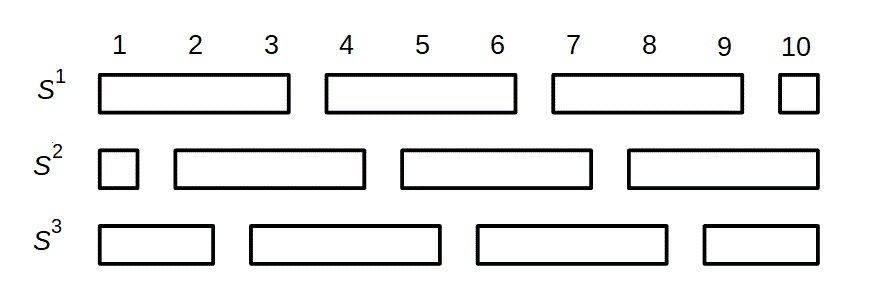
\includegraphics[scale=0.5]{slidingwindow2.jpg}
\caption{The three solutions for $T_0=3$ and $T=10$.}\label{fig:solutions}
\end{center}
\end{figure}


More formally, given an $\epsilon>0$, the algorithm $PTAS_{MK}$ works as follows.
\begin{itemize}
\item Let $\epsilon'=\epsilon/2$ and $T_0=\left\lceil \frac{1}{\epsilon'}\right\rceil$. Let ${\cal I}_t=[t,\dots, t+T_0-1] \cap [1, \dots, T]$ be the  set of (at most) $T_0$ consecutive time steps starting at $t$. We consider ${\cal I}_t$ for any $t$ for which it is non empty (so $t\in [-T_0+2 \dots T]$).%. Divide the $T$ time steps into $\frac{T}{T_0}$ time intervals \footnote{For ease of notation we assume that $T$ is a multiple of $T_0$. Otherwise, we can add at most $T_0$ dummy steps with both profits and bonuses equal to 0.} $I_t$ corresponding to the interval $[t, t+1, \ldots, t+T_0-1]$.
\item For $t \in \{1, \ldots, T_0 \}$:
\begin{itemize}
    \item Apply $A_{\epsilon',T_0}$ on all intervals ${\cal I}_{t'}$ with $t'\equiv t \pmod{T_0}$.
    %${\cal I}_{t+kT_0}$. 
    Note that each time step belongs to exactly one of such intervals. %, I_{t+T_0},I_{t+2T_0},\ldots, I_{t+T-T_0}$
    \item Define the solution $S^t$ built from the partial solutions given by the applications of $A_{\epsilon'\textbf{},T_0}$.
\end{itemize}
\item Choose the best solution $S$ among the $T_0$ solutions $S^1,\dots,S^{T_0}$.
\end{itemize} 

%The construction is illustrated on Figure~\ref{fig:solutions}, with 10 time steps and $T_0=3$. The first solutions $S^1$ is built by applying  4 times $A_{\epsilon,T_0}$, on the subinstances corresponding to time steps $\{1,2,3\}$, $\{4,5,6\}$, $\{7,8,9\}$, and $\{10\}$.


\begin{theorem}\label{thptasgen}
The algorithm $PTAS_{MK}$ is a polynomial time approximation algorithm.
\end{theorem}



\begin{proof}
The algorithm calls the $A_{\epsilon',T_0}$ algorithm $\lceil T/T_0 \rceil$ times for each of the $T_0$ generated solutions. Yet, the running time of  $A_{\epsilon',T_0}$ is  $n^{f(\frac{1}{\epsilon'},T_0)}=n^{f(\frac{2}{\epsilon},\lceil \frac{2}{\epsilon}\rceil)}$, i.e a polynomial time for any fixed $\epsilon$.  So, the running time of the algorithm for any $T$ is\\ $T_0\times \left \lceil \frac{T}{T_0} \right \rceil n^{f(\frac{2}{\epsilon},\frac{2}{\epsilon})} = O(T n^{f(\frac{2}{\epsilon},\frac{2}{\epsilon})})$, a polynomial time for any fixed $\epsilon$. \\

Each solution $S^t$ of the $T_0$ generated solutions may loose some bonus between the last time step of one of its intervals ${\cal I}_{t+kT_0}$ and the first time step of its next interval ${\cal I}_{t+(k+1)T_0}$ (in Figure~\ref{fig:solutions} for instance, $S^1$ misses the bonuses between steps 3 and 4, 6 and 7, and 9 and 10). Let $loss(S^t)$ be this loss with respect to some optimal solution $S^*$. Since we apply $A_{\epsilon',T_0}$ to build solutions, we get that the value $g(S^t)$ of $S^t$ is such that:

$$g(S^t)\geq (1-\epsilon') g(S^*) - loss(S^t)$$

Since the output solution $S$ is the best among the solutions $S^t$, by summing up the previous inequality for $t=1,\dots,T_0$ we get:

$$g(S)\geq (1-\epsilon') g(S^*)-\frac{\sum_{t=1}^T loss(S^t)}{T_0}$$

Now, by construction the bonus between steps $j$ and $j+1$ appears in the loss of  exactly one $S^t$ (see Figure~\ref{fig:solutions}). So the total loss of the $T_0$ solutions is the global transition bonus of $S^*$, so at most $g(S^*)$. Hence:

\begin{eqnarray*}
g(S) &\geq &  (1-\epsilon')g(S^*)-\frac{g(S^*)}{T_0} \\
&\geq&(1-2\epsilon')g(S^*) = (1-\epsilon) g(S^*)
\end{eqnarray*} 


\end{proof}

%Due to space constraints, the proof of Theorem~\ref{thptasgen} is deferred to Appendix (section~\ref{appthptasgen}). The underlying idea is to upper bound the loss of the algorithm which corresponds to transition costs between time steps $aT_0$ and $aT_0+1$, for $1\leq a\leq q-1$. 

\section{Pseudo-polynomiality and hardness results}

We complement the previous result on approximation scheme by showing the following results for {\sc Multistage  Knapsack}:
\begin{itemize}
\item First, it does not admit an FPTAS (unless \textbf{P=NP}), even if there are only two times steps (Section~\ref{sec:nofptas}) and the bonus is uniform ($B_{ti}=B$ for all $i$, all $t$);
\item Second, the problem is pseudo-polynomial if the number of time steps $T$ is a fixed constant (Section~\ref{sec:pseudo}) but is strongly \textbf{NP}-hard in the general case even in the case of uniform bonus (Section~\ref{sec:strong}). 
\end{itemize}

%In this section, the proof are made in an easier setting where the bonus is a fixed constant called $B$.  

\subsection{No FPTAS}\label{sec:nofptas}



\begin{theorem}\label{thnofptas}
There is no $FPTAS$ for {\sc Multistage Knapsack} unless \textbf{P=NP}, even if there are only two time steps and the bonus is uniform.
\end{theorem}
\begin{proof}
We prove the result by a reduction from CARDINALITY$(2-KP)$, known to be \textbf{NP}-complete (Theorem~ \ref{th:dimkp}) 

For an instance $I$ of CARDINALITY$(2-KP)$, we consider the following instance $I'$ of {\sc Multistage  Knapsack}: \\
\begin{itemize}
\item There are $T=2$ time steps, and the same set of objects $N=\{1,2,...,n\}$ as in $I$.
\item The weights $w_{1i}$ and $w_{2i}$ are the same as in $I$, for all $i \in N$.
\item $p_{1i}=p_{2i}=1$ for all $i \in N$.
\item $B_{1i}=2$ for all $i\in N$.
\end{itemize}

We show that the answer to $I$ is Yes (we can find $K$ objects fulfilling the 2 knapsack constraints) if and only if there is a solution of value at least $2K+2n$ for the instance $I'$ of $MK$.

If we have a set $A$ of $K$ objects for $I$, then we simply take these objects at both time steps in $I'$. This is feasible, the knapsack revenue is $2K$ and the transition revenue is $2n$.

Conversely, consider an optimal solution of value at least $2K+2n$ in $I'$. In an optimal solution, we necessarily have $x_{1j}=x_{2j}$, i.e an object is taken at the time $1$ if and only if it is taken at the time $2$. Indeed, assume that there is one $i \in N$ such that $x_{1i} \neq x_{2i}$, then consider the solution where $x_{1i} = x_{2i}=0$. This is still feasible; the knapsack revenue reduces by 1 but the transition revenue increases by $2$, contradiction.
Thus the same set of objects $A$ is taken at both time steps. Since the value of the solution is at least $2K+2n$, the size of $A$ is at least $K$. Hence the answer to $I$ is Yes.

Note that in $I'$ the optimal value is at most $4n$. We produce in this reduction polynomially bounded instances of {\sc Multistage  Knapsack} (with only two time steps), so the problem does not admit an FPTAS. Indeed, suppose that there is an FPTAS producing a $(1-\epsilon)$-approximation in time $p(1/\epsilon,n)$, for some polynomial $p$. Let $\epsilon = \frac{1}{4n+1}$. If we apply the FPTAS with this value of $\epsilon$ on $I'$ we get a solution $S$ of value at least  $(1-\epsilon)OPT(I')\geq OPT(I') - \frac{OPT(I')}{4n+1} > OPT(I')-1$. Yet all the possible values are integers so $S$ is optimal. The running time is polynomial in $n$, impossible unless \textbf{P=NP}.
\end{proof} 



\subsection{Pseudo-polynomiality for a constant number of time steps}\label{sec:pseudo}

We show here that the pseudo-polynomiality of the {\sc Knapsack} problem generalizes to {\sc Multistage  Knapsack} when the number of time steps is constant. More precisely, with a standard dynamic programming procedure, we have the following.

\begin{theorem}\label{thpseudo}
{\sc Multistage  Knapsack} is solvable in time $O(T(2C_{max}+2)^Tn)$ where $C_{max}=\max\{C_i,i=1,\dots,T\}$.
\end{theorem}


\begin{proof}

For any $T$-uple $(c_1,\dots,c_T)$ where $0\leq c_i\leq C_i$, and any $s\in \{0,\dots,n\}$, we define $\alpha(c_1,\dots,c_T,s)$ to be the best value of a solution $S=(S_1,\dots,S_T)$ such that:
\begin{itemize}
	\item The weight of knapsack at time $t$ is at most $c_t$: for any $t$, $\sum_{i\in S_t}w_{ti}\leq c_i$;
	\item The solution uses only objects among the first $s$: for any $t$, $S_t\subseteq \{1,\dots,s\}$.
\end{itemize}
The  optimal value of {\sc Multistage  Knapsack} is then $\alpha(C_1,\dots,C_T,n)$. We compute $\alpha$ by increasing values of $s$. For $s=0$, we cannot take any object so $\alpha(c_1,\dots,c_T,0)=0$. 

Take now $s\geq 1$. To compute $\alpha(c_1,\dots,c_T,s)$, we simply consider all the $2^T$ possibilities for taking or not object $s$ in the $T$ time steps. Let $A\subseteq \{1,\dots,T\}$ be a subset of time steps. If we take object $s$ at time steps in $A$ (and only there), we first check if $A$ is a {\it valid} choice, i.e., $w_{ts}\leq c_t$ for any $t\in A$; then we can compute in $O(T)$ the corresponding reward $r_s(A)$ ($\sum_{t\in A}p_{ts}$ plus the transition bonus). We have:

$$\alpha(c_1,\dots,c_T,s)=$$
$$\max\{r_s(A)+\alpha(c_1-w_{1s},\dots,c_T-w_{Ts},s-1):A\subseteq\{1,\dots,T\} \mbox{ valid}\}$$

The running time to compute one value of $\alpha$ is $O(T2^T)$. There are $O(n\Pi_{t=1}^T(C_i+1))=O(n(C_{max}+1)^T)$ values to compute, so the running time follows. A standard backward procedure allows to recovering the solution.
\end{proof}



%Due to space constraints, the proof of Theorem~\ref{thpseudo} is deferred to the Appendix (Section~\ref{appthpseudo}).

\subsection{Strongly NP-hardness}\label{sec:strong}

\begin{definition}
{\sc Binary Multistage  Knapsack}  is the sub-problem of the Multistage {\sc Knapsack} where all the weights, profits and capacities are all equal to 0 or $1$.
\end{definition}


For the usual {\sc Knapsack} problem, the binary case corresponds to a trivial problem. For the multistage case, we have the following: 

\begin{theorem}
{\sc Binary Multistage  Knapsack} is \textbf{NP}-hard, even in the case of uniform bonus.
\end{theorem}

\begin{proof}


We prove the result by a reduction from the {\sc Independent Set} problem where, given a graph $G$ and an integer $K$, we are asked if there exists a subset of $K$ pairwise non adjacent vertices (called an independent set). This problem is well known to be \textbf{NP}-hard, see \cite{gj}.  


Let $(G,K)$ be an instance of the  {\sc Independent Set} problem, with $G=(V,E)$, $V=\{v_1,\dots,v_n\}$ and $E=\{e_1,\dots,e_m\}$. We build the following instance $I'$ of {\sc Binary Multistage  Knapsack}: 
\begin{itemize}
\item There are $n$ objects $\{1,2\dots,n\}$, one object per vertex;
\item There are $T=m$ time steps: each edge $(v_i,v_j)$ in $E$ corresponds to one time step;
\item at the time step corresponding to edge $(v_i,v_j)$: objects $i$ and $j$ have weight 1, while the others have weight 0, all objects have profit 1, and the capacity constraint is 1.
\item The transition profit is $b_{ti}=B=2nm$ for all $i,t$.
\end{itemize}

We claim that there is an independent set of size (at least) $K$ if and only if there is a solution for {\sc Binary Multistage  Knapsack} of value (at least) $n(m-1)B+mK$. 

Suppose first that there is an independent set $V'$ of size at least $K$. We take the $K$ objects corresponding to $V'$ at all time steps. This is feasible since we cannot take 2 objects corresponding to one edge. The built solution sequence has knapsack profit $mK$ and transition profit $n(m-1)B$ (no modification). 

Conversely, take a solution of {\sc Binary Multistage  Knapsack} of value at least $n(m-1)B+mK$. Since $B=2nm$, there must be no modification of the knapsack over the time. Indeed, otherwise, the transition profit would be at most $n(m-1)B-B$, while the knapsack profit is at most $mn$, so the value would be less than $n(m-1)B$. So we consider the set of vertices corresponding to this knapsack. Thanks to the value of the knapsack, it has size at least $K$. Thanks to the capacity constraints of the bags, this is an independent set. 
\end{proof}
Since $B$ is polynomially bounded in the proof, this shows that {\sc Multistage  Knapsack} is strongly \textbf{NP}-hard.
\section{Conclusion}
We considered the {\sc Multistage Knapsack} problem in the offline setting and we studied the impact of the number of time steps in the complexity of the problem. In the next chapter, we present the study in the online setting of the large family of subset maximization problems in the multistage framework, the {\sc multistage knapsack} problem being part of this family, and measure the importance of the knowledge of the future on the quality of solutions.
%SFS is studied in Section~\ref{sec:static}, while GE in Section~\ref{sec:general}.

%\subsubsection{On-line competitive analysis and model with lookahead}
%ADDED SOME LINES see lines 46-52

%To be said: 

%- on-line setting (we have to decide $S_t$ without knowing $I_{t'}$ for $t'>t$.

%- Competitive analysis: notion of asymptotic ratios (both for upper and lower bounds). Also a word on the fact that we require to be competitive only at the end (time $T$)

%- In the case where there is no competitive ratio in particular: model of lookahead. $k$ lookahead.

%Also somewhere: lower bounds given for knapsack, arguably one of the most simple problems of this class (the set of feasible solutions is defined as a single linear constraint).
\label{}

%% The Appendices part is started with the command \appendix;
%% appendix sections are then done as normal sections
%% \appendix

%% \section{}
%% \label{}

%% If you have bibdatabase file and want bibtex to generate the
%% bibitems, please use
%%
\chapter{Online Multistage Subset Maximisation Problems} \label{chap:onlmultista}
\chaptermark{}

\section{Introduction}

%In a classical combinatorial optimization setting, given an instance of a problem one needs to find a good feasible solution. However, in many situations, the data may evolve over time and one has to solve a sequence of instances. The natural approach of solving every instance independently may induce a significant transition cost, for instance for moving a system from one state to another. This cost may represent, e.g., the cost of turning on/off the servers in a data center \cite{LinWAT13,BansalGKPSS15,AntoniadisS17,AlbersQ18}, the cost of changing the quality level in video streaming \cite{Joseph}, or the cost for turning on/off nuclear plants \cite{thesececile}.  %It becomes then necessary to study optimization problems in a new framework where the objective is to know whether it is possible to determine  a tradeoff between the quality of the solutions in each time step and the stability/similatity of the solutions in cosnecutive time steps.  
%Gupta et al. \cite{Gupta} and Eisenstat et al. \cite{Eisenstat}  proposed
% a \emph{multistage} model where given  a time horizon $t = 1, 2, \ldots,T$,  the input is a sequence of instances $I_1,I_2,\ldots,I_T$, (one for each time step), and the goal is to find a sequence of solutions $S_1,S_2,\ldots,S_T$ (one for each time step) reaching  a trade-off between the quality of the solutions in each time step and the stability/similarity of the solutions in consecutive time steps. The addition of the transition cost makes some  classic combinatorial optimization problems much harder. This is the case  for instance  %some problems (e.g. 
 %for the minimum weighted perfect matching problem in the \emph{off-line} case where the whole sequence of instances is known in advance. While the one-step problem is polynomially-time solvable, the multistage problem becomes hard to approximate even for bipartite graphs and for only two time steps \cite{Bampis,Gupta}. 
 
 In this chapter, we focus on the online  case, where at time $t$ no knowledge is available for instances at times $t+1, \ldots, T$.  When it is not possible to handle the online case, we turn our attention to the $k$-\emph{lookahead} case, where at time $t$ the instances at times $t+1, \ldots, t+k$ are also known. This case is of interest since in some applications like in  dynamic capacity planning in data centers,
 the forecasts of future demands may be very helpful (see \cite{Lin,Liu} for examples of application). 
 Our goal is to measure the impact of the lack of knowledge of the future  on the quality and the stability of the returned solutions. 
 Indeed, our algorithms are limited in their knowledge of the sequence of instances.
Knowing that the number of time steps is given, we compute the competitive ratio of the algorithm after time step $T$: As we focus on maximization problems, we say that a \finalversion{(deterministic)} algorithm is $\alpha$-competitive (with competitive ratio $\alpha$) if its value is at least $\frac1\alpha$ times the optimal value on all instances.

As it is usual in the online setting, we consider no limitations in the computational resources available. This implies that at every time step $t$, where instance $I_t$ is known, we assume the existence of an oracle able to compute the optimal solution for that time step.  Notice also that our lower bounds do not rely on any complexity assumptions. 
Some recent results are already known for the online multistage model (\cite{Bampis+,Gupta}), however all these results are obtained for specific problems.
In this chapter, we study multistage variants  of a broad family of maximization problems. An extended abstract of this chapter has been presented at ESA (European Symposium on Algorithms) 2019 (\cite{BampisEST19}).

\subsection{Problem definition}
The family of optimization problems that we consider is the following. 
 
 

\begin{definition}

\emph{(Subset Maximization Problems.)} A Subset Maximization problem $\cal P$ is a combinatorial optimization problem whose instances $I=(N,p,\mathcal{F})$ consist of
\begin{itemize}
    \item A ground set $N$;
    \item A set $\mathcal{F}\subseteq 2^N$ of feasible solutions such that $\emptyset\in\mathcal{F}$;
    \item A non-negative weight $p(S)$ for every $S \in \mathcal{F}$.
\end{itemize}
The goal is to find $S^*\in \mathcal{F}$ such that $p(S^*)=\max\{p(S):S\in\mathcal{F}\}$.
\end{definition}
We will consider that the empty set is always feasible, ensuring that the feasible set of solutions is non empty.
This is a very general class of problems, including the maximization \emph{Subset Selection} problems studied by \cite{Pruhs} (they only considered linear objective functions). It contains for instance graph problems where $N$ is the set of vertices (as in any maximization induced subgraph problem verifying some property) or the set of edges (as in  matching problems). It also contains classical set problems (knapsack, maximum 3-dimensional matching,\dots), and more generally 0-1 linear programs (with non negative profits in the objective function).



Given a problem in the previous class, we are interested in its multistage version~(\cite{Gupta,Eisenstat}).
The stability over time of a solution sequence is classically captured by considering a transition cost when a modification is made in the solution. Here, dealing with maximization problems as in the previous chapter, we will consider again a transition {\it bonus} $B$ for taking into account the similarity of two consecutive solutions.
In what follows, we will use the term object to denote an element of $N$ (so an object can be a vertex of a graph, or an edge,\dots, depending on the underlying problem). 	%\textcolor{red}{Kevin: were we assuming anywhere now that $\emptyset$ is feasible?}

\begin{definition}
\emph{(Multistage Subset Maximization Problems.)} In a Multistage Subset Maximization problem $\cal P$, we are given
\begin{itemize}
\item a number of steps $T \in \mathbb{N}$, a set $N$ of $n$ objects;
\item for any $t \in T$, an instance $I_t$ of the optimization problem. We will denote:
\begin{itemize}
\item $p_{t}$ the objective (profit) function at time $t$
\item $\mathcal{F}_t\in 2^N$ the set of feasible solutions at time $t$
\end{itemize} 
%\item For each $t$: $C_t$ the capacity of knapsack at time $t$
\item $B \in \mathbb{R^{+}}$ a given transition profit. 
\item the value of a solution sequence $\mathcal{S}=(S_1,\dots,S_T)$ is %$$f(\mathcal{S})=\sum_{t=1}^T p_t(S_t) + \sum_{t=1}^{T-1} b(S_t,S_{t+1})$$
\[f(\mathcal{S})=\sum_{t=1}^T p_t(S_t) + \sum_{t=1}^{T-1} b(S_t,S_{t+1})\]


where $b(S_t,S_{t+1})$ is the transition bonus for the solution between time steps $t$ and $t+1$. We will use the term {\it profit} for $ p_t(S_t)$, {\it bonus} for the transition bonus $b(S_t,S_{t+1})$, and {\it value} of a solution $\mathcal{S}$ for $f(\mathcal{S})$;
\item the goal is to determine a solution sequence of maximum value. 
\end{itemize}
\end{definition}

\finalversion{The fact that $T$ is known may be regarded as rather uncommon the field of online algorithms. At the end of Subsection~\ref{subsec:results}, we relate it to our results and justify it.}

 There are two natural ways to define the transition bonus. We will see that these two ways of measuring the stability induce some differences in the competitive ratios one can get. 

\begin{definition}
\emph{(Types of transition bonus.)}
 If $S_t$ and $S_{t+1}$ denote, respectively, the solutions for time steps $t$ and $t+1$, then we can define the transition bonus as:
\begin{itemize}
    \item \emph{Intersection Bonus:}  $B$ times $|S_{t}\cap S_{t+1}|$: in this case the bonus is proportional to the number of objects in the solution at time $t$ that remain in it at time $t+1$.
    \item \emph{Hamming Bonus:} $B$ times $|S_{t}\cap S_{t+1}|+|\overline{S_{t}}\cap \overline{S_{t+1}}|$. Here we get the bonus for each object for which the decision (to be in the solution or not) is the same between time steps $t$ and $t+1$. In other words, the bonus is proportional to $|N|$ minus the number of modifications (Hamming distance) in the solutions. The {\sc multistage knapsack} problem was studied considering \emph{Hamming Bonus} in the chapter \ref{chap:multiknap}. 
\end{itemize}
\end{definition}

Note that by scaling profits (dividing them by $B$), we can arbitrarily fix $B=1$. So from now on, we assume $B=1$. Note that this was also the case with the uniform bonus presented in the chapter \ref{chap:multiknap}.

%Note that we may allow $w_{ti}>C_t$: this may model the fact that object $i$ is not available at time $i$.\\

%\subsubsection{Models of evolution}

In this chapter, we will consider two possible ways for the data to evolve. 

\begin{definition}
\emph{(Types of data evolution.)}
\begin{itemize}
\item \emph{Static Set of Feasible Solutions (SSFS):}  only profits may change over time, so the structure of feasible solutions remains the same: $\mathcal{F}_t=\mathcal{F}$ for all $t$. 

\item \emph{General Evolution (GE):}  any modification (but the set of objects) in the input sequence is possible. Both the profits and the set of feasible solutions may change over time. In this latter model, for knapsack, profits and weights of object (and the capacity of the bag) may change over time; for maximum independent set edges in the graph may change,\dots.   
\end{itemize}
\end{definition}


\subsection{Summary of Results and Overview}\label{subsec:results}

The contribution of this chapter is a framework for online multistage maximization problems (comprising different models) and almost tight upper and lower bounds on the best-possible competitive ratio for these models. \finalversion{The focus here is on deterministic algorithms.}

We increase the complexity of the considered models over the course of the chapter. We start with the arguably simplest model: Considering a static set of feasible solutions clearly restricts the general model of evolution; while such a straightforward comparison between the Hamming and intersection bonus is not possible, the Hamming bonus seems simpler in that, compared to the intersection model, there are (somewhat comparable) extra terms added on the profit of both the algorithm and the optimum. As we show in Subsection~\ref{subsec:static-hamming}, there is indeed a simple $2$-competitive algorithm: At each time $t$, it greedily chooses the set $S_t$ that either maximizes the transition bonus w.r.t.\ $S_{t-1}$ (that is, choosing $S_t=S_{t-1}$, which is possible in this model) or maximizes the value $p_t(S_t)$. We complement this observation with a matching lower bound only involving two time steps.

We then toggle the transition-bonus model and the data-evolution model separately and show that constant competitive ratios can still be achieved. First, in Subsection~\ref{subsec:static-intersection}, we consider intersection bonus. We show that, \emph{after} modifying the profits \finalversion{(internally)} to make larger solutions more profitable, a $(2+1/(T-1))$-competitive algorithm can be achieved by a greedy approach again. We also give an (almost matching) lower bound of $2$ again. Next, we toggle the evolution model. In Subsection~\ref{subsec:general-hamming}, we adapt the greedy algorithm from Subsection~\ref{subsec:static-hamming} by reweighting to obtain a $(3+1/(T-1))$-competitive algorithm using a more complicated analysis. We complement this result with a lower bound of $1+\sqrt{2}$.

In Subsection~\ref{subsec:general-intersection}, we finally consider the general-evolution model with intersection bonus, where we give a simple lower bound showing that a constant-competitive ratio is not achievable. This lower bound relies on forbidding to choose any item in the second step that the algorithm chose in the first step. We circumnavigate such issues by allowing the algorithm a lookahead of one step and present a $4$-competitive algorithm for that setting. A similar phase transition has been observed for a related problem~ (\cite{Bampis+}), but our algorithm, based on a doubling approach, is different. We also give a matching lower bound of $4$ on the competitive ratio of any algorithm in the same setting. We summarize all results described thus far in Table~\ref{table:resultsMultiSub}.



\begin{table}[t]
	\centering
	\def\arraystretch{1.1}
	\begin{tabular}{ccc}
		\toprule
		&static set of feasible solutions&general evolution\\
		\midrule
		% Bounds hamming bonus
		\multirow{2}{*}{Hamming bonus}& \finalversion{$2-o(1)\leq c^\star\leq2$} & $1+\sqrt{2}\leq c^\star\leq3+o(1)$ \\
		% References hamming bonus
		&  Theorems \ref{thm:static-hamming-lower} and \ref{thm:static-hamming-upper} & Theorems \ref{thm:general-hamming-lower} and \ref{thm:general-hamming-upper}\\[1ex]  
		\midrule
		% Bounds intersection bonus
		\multirow{3}{*}{Intersection bonus}& \multirow{2}{*}{$2\leq c^\star\leq 2+o(1)$} & $c^\star=\infty$\\
		& & $c^\star=4$ for $1$-lookahead\\		
		% References intersection bonus
		&  Theorems \ref{thm:static-intersection-lower} and \ref{thm:static-intersection-upper} & Theorems \ref{thm:general-intersection-lower}, \ref{thm:general-intersection-lower1}, and \ref{thm:general-intersection-upper} \\[1ex]  
		\bottomrule
	\end{tabular}
	\medskip
	\caption{Our bounds on the best-possible competitive ratio $c^\star$ for the different models. The Landau symbol is with respect to $T\rightarrow\infty$.}
	\label{table:resultsMultiSub}
\end{table}

We note that the lower bounds mentioned for the Hamming model are only shown for a specific fixed number of time steps, and that in general there is no trivial way of extending these bounds to a larger number of time steps. 
%Only in the model with general evolution and intersection bonus, one can add extra time steps (in which only the empty set is feasible and has no profit) that neither add to the algorithm's nor the optimum's profit.
One may however argue that the large-$T$ regime is in fact the interesting one for both practical applications and in theory, the latter because the effect of having a first time step without bonus vanishes. At the end of the respective sections, we therefore give asymptotical lower bounds of $3/2$ and roughly $1.696$ for the cases of a static set of feasible solutions and general evolutions, respectively. These bounds are non-trivial, but we do not know if they are tight.

It is plausible that the aforementioned upper bounds can be improved if extra assumptions on characteristics of the objective function and the sets of feasible solutions are made. In Subsubsection~\ref{subsec:submodular}, we show that already very natural assumptions suffice: Assuming that at each time the feasible solutions are closed under taking subsets and the objective function is \finalversion{subadditive}, we give a $(21/8+o(1))$-competitive algorithm for the model with a general evolution and Hamming bonus, improving the previous $(3+o(1))$-competitive ratio. Our  lower bounds for general evolution and Hamming bonus in fact fulfill the extra assumptions.

\finalversion{We observe that all our algorithms except for the one discussed in Subsection~\ref{subsec:static-hamming} require that $T$ is known in that their behavior in the last step is different from the behavior in the steps before. This assumption is crucial: In all these models, there are examples in which one can in the first time step choose either a small profit or a potentially large bonus not knowing if there is another timestep to realize the bonus. Such examples imply a superconstant lower bound on the competitive ratio in these models. This justifies our assumption that $T$ is known.}

In Section~\ref{sec:conclusion}, we summarize our results and mention directions for future research that we consider interesting.

%Due to space constraints, some proofs only appear in the full version~\cite{abs-1905-04162}.


\section{Model of a Static Set of Feasible Solutions}\label{sec:staticFea}

We consider here the model of evolution where only profits change over time: $\mathcal{F}_t=\mathcal{F}$ for any~$t$. 
We first consider the Hamming bonus model and show a simple 2-competitive algorithm. We will then show that a (asymptotic) competitive ratio of 2 can also be achieved in the intersection bonus model using a more involved algorithm. In both cases, this ratio 2 is shown to be (asymptotically) optimal.  

\subsection{Hamming-Bonus Model}
\label{subsec:static-hamming}

\begin{theorem}\label{thm:static-hamming-upper}
In the SSFS model with Hamming bonus, there is a 2-competitive algorithm. 
\end{theorem}

\begin{proof}
We consider the very simple following algorithm. At each time step $t$, the algorithm computes an optimal solution $S^*_t$ with associated profit $p_t(S^*_t)$. At $t=1$ we fix $S_1=S^*_1$. For $t>1$, if $p_t(S^*_t) > n$ then fix $S_t=S^*_t$, otherwise fix $S_t=S^*_{t-1}$ (which is possible thanks to the fact that the set of feasible solutions does not change).

Let $f^*$ be the optimal value. Since any solution sequence gets profit at most $p_t(S^*_t)$ at time $t$, and bonus at most $n$ between two consecutive time steps, we get $f^* \leq \sum_{t=1}^T p(S^*_t) + n(T-1)$. 

By construction, at time $t>1$, either the algorithm gets profit $p_t(S^*_t)$ when $p_t(S^*_t)>n$, or bonus (from $t-1$) $n$ when $n\geq p_t(S^*_t)$. So in any case the algorithm gets profit plus bonus at least $\frac{p_t(S^*_t)+n}{2}$. At time $1$ it gets profit at least $p_1(S^*_1)$. So 
%$$f(S_1\dots,S_T)\geq p_1(S^*_1)+\sum_{t=2}^T \frac{p_t(S^*_t)}{2}+ \frac{n(T-1)}{2}\geq \frac{f^*}{2},$$
\[f(S_1\dots,S_T)\geq p_1(S^*_1)+\sum_{t=2}^T \frac{p_t(S^*_t)}{2}+ \frac{n(T-1)}{2}\geq \frac{f^*}{2} \]
which completes the proof. %\qed  
\end{proof}

\begin{theorem}\label{thm:static-hamming-lower}
Consider the SSFS model with Hamming bonus. For any $\epsilon>0$, there is no $(2-\epsilon)$-competitive algorithm, even if there are only $2$ time steps. 
\end{theorem}

\begin{proof}
We consider a set $N=\{1,2,\dots,n\}$ of $n=1+\left\lceil \frac{1}{\epsilon}\right\rceil$ objects, $T=2$ time steps, \finalversion{and an additive profit function}. There are three feasible solutions: $S^0=\emptyset$, $S^1=\{1\}$ and $S^2=\{2,\dots,n\}$. At $t=1$, all the profits are 0. Let us consider an online algorithm \texttt{A}. We consider the three possibilities for the algorithm at time 1:
\begin{itemize}
\item At time 1, \texttt{A} chooses $S^0$: at time 2 we give profit 1 to all objects. If \texttt{A} takes no object at time 2, it gets profit 0 and bonus $n$. If it takes $S^1$, it gets profit 1 and bonus $n-1$. If it takes $S^2$, it gets profit $n-1$ and bonus 1, so in any case the computed solution has value $n$. The solution consisting of taking $S^2$ at both time steps has profit $n-1$ and bonus $n$, so value $2n-1$.
\item At time 1, \texttt{A} chooses $S^1$: at time 2 we give profit 0 to object 1, and profit 1 to all other objects. Then, if the algorithm takes $S^0$ (resp, $S^1$, $S^2$), at time 2 its gets value $n-1$ (resp, $n$, $n-1$) while the solution consisting of taking $S^2$ at both time steps has value $2n-1$.
\item At time 1, \texttt{A} chooses $S^2$: at time 2 we give profit $n$ to object 1, and 0 to all other objects. Then if the algorithm takes $S^0$ (resp, $S^1$, $S^2$) at time 2 its gets value \finalversion{$1$} (resp, $n$, $n$), while  the solution consisting of taking $S^1$ at both time steps has value $2n$.
\end{itemize}
In any case, the ratio is at least $\frac{2n-1}{n}=2-\frac{1}{n}>2-\epsilon$. %\qed 
\end{proof}

We complement this lower bound with an asymptotical result for large $T$.%; the proof is provided in the full version.
%; the proof is provided in the appendix.

\begin{theorem}\label{th:lbmod1}
	Consider the SSFS model with Hamming bonus. For every $\epsilon>0$, there is a $T_\epsilon$ such that, for each number of time steps $T\geq T_\epsilon$, there is no $(3/2-\epsilon)$-competitive algorithm.
\end{theorem}

\begin{proof}
	Let $N:=\{1,2\}$. The static set of feasible solutions is $\mathcal{F}=\{\emptyset,\{1\},\{2\}\}$. Initially, $p_1(\{1\})=0$ and $p_1(\{2\})=1$. As long as the algorithm has not picked item $1$ until some time $t$, we set $p_{t+1}(\{1\})=0$ and $p_{t+1}(\{2\})=1$ again. Note that, in order to be $(3/2-\epsilon)$-competitive, the algorithm however has to pick item $1$ eventually. Further, the ratio between the profit of the optimum and the algorithm during this part is $3/2-o(1)$ as the length of this part approaches $\infty$.
	
	The remaining time horizon is partitioned into contiguous \emph{phases}. Consider a phase that starts at time $t$. The invariant at the beginning of the phase is that both the algorithm and the optimum have picked the same item in the previous time step $t-1$. Let this item be w.l.o.g.\ item $2$; the other case is symmetric. Then $p_t(\{2\})=1$ and $p_t(\{1\})=3$. By the same reasoning as above, we can assume the algorithm chooses an item at $t$. Let $i\in\{1,2\}$ be that item. Then $p_{t+1}(\{i\})=0$ and $p_{t+1}(\{3-i\})=1$. As long as the algorithm is still not picking item $3-i$ during the time interval $[t+1,t']$, $p_{t'+1}(\{i\})=0$ and $p_{t'+1}(\{3-i\})=1$. Once the algorithm picks item $3-i$ at some time, the phase ends \emph{regularly}; otherwise it ends \emph{by default}.
	
	Now consider a phase of length $\ell$ that ends regularly (note $\ell\geq 2$). We claim that the values of the algorithm and the optimum have a ratio of at least $3/2$. This is because of the following estimates on the algorithm's and optimum's value:
	\begin{itemize}
	    \item In either case for $i$, the algorithm obtains a value of $3$ in time step $t$. Furthermore, the total bonus in all subsequent time steps is $(\ell-2)\cdot 2$, because the algorithm has to switch from item $i$ to item $3-i$. There is an additional profit of $1$ at time $t+\ell-1$. Therefore, the total value is $4+(\ell-2)\cdot 2$
	    \item The value of the optimum is at least $6+(\ell-2)\cdot 3$: It chooses item $3-i$ already at time $t$ and keeps it until time $t+\ell-1$, obtaining a value of $3$ in that time step and another $3$ in each subsequent time step.
	\end{itemize}
	This proves the claim and thereby the theorem as a phase that ends by default can be extended to one that ends regularly by modifying the optimum's and algorithm's values by constants. %\qed 
\end{proof}

\subsection{Intersection Bonus Model}
\label{subsec:static-intersection}

In the Intersection Bonus model things get harder since an optimal solution $S^*_t$ may be of small size and then gives very small (potential) bonus for the next step. As a matter of fact, the algorithm of the previous section has unbounded competitive ratio in this case: take a large number $n$ of objects, $\mathcal{F}=2^N$, and at time 1 all objects have profit 0 up to one which has profit $\epsilon$. The algorithm will take this object (instead of taking $n-1$ objects of profit 0) and then potentially get bonus at most 1 instead of $n-1$.

Thus we shall put an incentive for the algorithm to take solutions of large size, in order to have a chance to get a large bonus. We define the following algorithm called \texttt{MP-Algo} (for Modified Profit algorithm). Informally, at each time step $t$, the algorithm computes an optimal solution with a modified objective function $p'_{t}$. These modifications take into account (1) the objects taken at time $t-1$ (2) an incentive to take a lot of objects. Formally, \texttt{MP-Algo} works as follows:

\begin{enumerate}
    \item At $t=1$: let $p'_{1}(S)=p_{1}(S)+|S|$. Choose $S_1$ as an optimal solution for the problem with modified profits $p'_{1}$. 
    \item For $t$ from 2 to $T-1$: let $p'_{t}(S)=p_{t}(S)+|S\cap S_{t-1}|+|S|$. Choose $S_t$ as an optimal solution for the problem  with modified profit function $p'_{t}$. 
    \item At $t=T$: let $p'_{T}(S)=p_{T}(S)+|S\cap S_{T-1}|$. Choose $S_T$ as an optimal solution with modified profit function $p'_{T}$. 
\end{enumerate}
The cases $t=1$ and $t=T$ are specific since there is no previous solution for $t=1$, and no future solution for $t=T$.

\begin{theorem}\label{thm:static-intersection-upper}
In the SSFS model with intersection bonus, \texttt{MP-Algo} is $\left(\frac{2}{1-1/(T-1)}\right)$-compe\-titive.
\end{theorem}

\begin{proof}

 Let $(\hat{S}_1,\dots,\hat{S}_T)$ be an optimal sequence. Since $S_t$ is optimal with respect to $p'_t$, for $t=2,\dots,T-1$ we have:
 \begin{equation}\label{eqBruno1}
 p'_t(S_t)=p_t(S_t)+|S_t\cap S_{t-1}|+|S_t|\geq p'_t(\hat{S}_t)\geq p_t(\hat{S}_t)+|\hat{S}_t|.
 \end{equation}
Since $S_{t-1}$ is also a feasible solution at time $t$, we have:
 \begin{equation}\label{eqBruno2}
 p'_t(S_t)=p_t(S_t)+|S_t\cap S_{t-1}|+|S_t|\geq p_t(S_{t-1}) \geq 2|S_{t-1}|.
 \end{equation}
Similarly, at $t=T$  $p'_T(S)=p_T(S)+|S\cap S_{t-1}|$ so 
 \begin{eqnarray}
 p_T(S_T)+|S_T\cap S_{T-1}| & \geq & p_T(\hat{S}_T), \label{eqBruno3}\\
  p_T(S_T)+|S_T\cap S_{T-1}|&\geq& |S_{T-1}|. \label{eqBruno4}
 \end{eqnarray}
At $t=1$, $p'_t(S)=p_t(S)+|S|$, so 
 \begin{equation}\label{eqBruno5}
 p_1(S_1)+|S_1|\geq p_1(\hat{S}_1)+|\hat{S}_1|.
 \end{equation}
Now, note that $|S_t\cap S_{t-1}|$ is the transition bonus of the computed solution between $t-1$ and~$t$. By summing Equation~(\ref{eqBruno1}) for $t=2,\dots,T-1$, Equation~(\ref{eqBruno3}) and Equation~(\ref{eqBruno5}), we deduce:
\begin{equation}\nonumber
    f(S_1,\dots,S_T)+\sum_{t=1}^{T-1}|S_t| \geq \sum_{t=1}^T p_t(\hat{S}_t)+\sum_{t=1}^{T-1}|\hat{S}_t|.
\end{equation}
Since in the optimal sequence the transition bonus between time $t$ and $t+1$ is at most $|\hat{S}_t|$, we get:
\begin{equation}\label{eqBruno6}
    f(S_1,\dots,S_T)+\sum_{t=1}^{T-1}|S_t| \geq f(\hat{S}_1,\dots,\hat{S}_T).
\end{equation}
Now we sum Equation~(\ref{eqBruno2}) for $t=2,\dots,T-1$ and Equation~(\ref{eqBruno4}):
\begin{equation}\nonumber
    f(S_1,\dots,S_T)+\sum_{t=2}^{T-1}|S_t| \geq 2\sum_{t=2}^{T-1}|S_{t-1}|+|S_{T-1}|.
\end{equation}
From this we easily derive:
\begin{equation}\label{eqBruno7}
    f(S_1,\dots,S_T) \geq \sum_{t=2}^{T-2}|S_{t}|.
\end{equation}
By summing Equations~(\ref{eqBruno6}) and~(\ref{eqBruno7}) we have $2f(S_1,\dots,S_T)\geq f(\hat{S}_1,\dots,\hat{S}_T)-|S_{T-1}|$. The competitive ratio follows from the fact that $f(\hat{S}_1,\dots,\hat{S}_T)\geq (T-1)|S_{T-1}|$ (since $S_{T-1}$ is feasible for all time steps). %\qed 
\end{proof}

We note that competitive ratio 2 can be derived with a similar analysis when 
the number of time steps is 2 or 3. Let us now show a matching lower bound (which is also valid in the asymptotic setting).

\begin{theorem}\label{thm:static-intersection-lower}
Consider the SSFS model with intersection bonus. For any $\epsilon>0$ and number of time steps $T=\lceil1/\epsilon\rceil$, there is no $(2-\epsilon)$-competitive algorithm.
\end{theorem}

\begin{proof}
Let $\epsilon>0$ and $T=\left\lceil \frac{1}{\epsilon}\right\rceil$. We consider $T$ time steps,  and a set $N$ of $n=T$ objects. The objective function is linear, and feasible solutions are sets of at most 1 object. At $t=1$, the profit of each object is 1. Then, at each time step, if the algorithm takes an object, this object will have profit 0 until the end. While an object is not taken by the algorithm, its profit remains 1.

Since the algorithm takes at most one object at each time step, there is an object which is never taken till the last step. The solution of taking this object during all the process has value $2T-1$. But at each time step the algorithm either takes a new object (and gets no bonus) or keeps the previously taken object and gets no profit. So the value of the computed solution is at most $T$. The ratio is $2-\frac{1}{T}\geq 2-\epsilon$. %\qed 
\end{proof}

%Note: we can get rid off the $-\frac{1}{T}$ in the lower bound by putting profit 0 at time 1 (and then 1 as in the previous construction). Then opt=$2(T-1)$ and algo $\leq T-1$. This gives LB of 2 asymptotic but also for any $T$ (eg. $T=2$).

\section{Model of General Evolution}\label{sec:general}

We consider in this section that the  set of feasible solutions may evolve over time. We will show that in the Hamming bonus model, we can still get constant competitive ratios, though ratios slightly worse than in the case where only profits could change over time. Then, we will tackle the intersection bonus model, showing that no constant competitive ratio can be achieved. However, with only $1$-lookahead we can get a constant competitive ratio.

\subsection{Hamming Bonus Model}
\label{subsec:general-hamming}

In this section we consider the Hamming bonus model. We first show in Section~\ref{subsec:general} that there exists a $\left(3+\frac{1}{T-1}\right)$-competitive algorithm.
Interestingly, we then show in Section~\ref{subsec:submodular} that a slight assumption on the problem structure allows to improve the competitive ratio. More precisely, we achieve a 21/8 (asymptotic) competitive ratio if we assume that the objective function is \finalversion{subadditive (so including the additive case)} and that a subset of a feasible solution is feasible. These assumptions are satisfied by all the problems mentioned in introduction.
We finally consider lower bounds in Section~\ref{sub:generallower}.

\subsubsection{General Case}\label{subsec:general}


We adapt the idea of the 2-competitive algorithm working for the Hamming bonus model for a static set of feasible solutions (Section~\ref{subsec:static-hamming}) to the current setting where the set of feasible solutions may change.  Let us consider the following algorithm \texttt{BestOrNothing}: at each time step $t$, \texttt{BestOrNothing} computes an optimal solution $S_t^*$ with associated profit $p_t(S_t^*)$ and compares it to $2$ times the maximum potential bonus, i.e to $2n$. It chooses $S^*_t$ if the associated profit is at least $2n$, otherwise it chooses $S_t=\emptyset$. A slight modification is applied for the last step  $T$. %We get the following result (proof omitted).
%, where it is a nonsense to compare a solution profit to the bonus if the algorithm chose to take a solution with objects at the time step $T-1$, since it does not get any transition bonus this way. 

Formally, \texttt{BestOrNothing}  works as follows: 

\begin{enumerate}
\item For $t$ from 1 to $T-1$:
\begin{enumerate}
	\item Compute an optimal solution $S^*_t$ at time $t$ with associated profit $p_t(S_t^*)$ 
	\item If $p_t(S_t^*)\geq 2n$ set $S_t=S^*_t$, otherwise set $S_t=\emptyset$.
\end{enumerate}
\item At time $T$:
	\begin{enumerate}
	\item if $S_{T-1}=S^*_{T-1}$, then $S_T=S^*_T$. 
	\item Otherwise: if $p_t(S_t^*)\geq n$ set $S_T=S^*_T$, otherwise set $S_T=\emptyset$.
	\end{enumerate}
\end{enumerate}

We show an upper bound on the competitive ratio achieved by this algorithm.

\begin{theorem}\label{thm:general-hamming-upper}
In the GE model with Hamming bonus, \texttt{BestOrNothing} is $\left(3+\frac{1}{T-1}\right)$-competitive.
\end{theorem}

\begin{proof}
Let us define $J\subseteq\{1,\dots,T-1\}$ as the set of time steps $t<T$ where $p_t(S_t^*)\geq 2n$. 

If $J\neq \emptyset$, let $t_1$ be the largest element in $J$. We first upper bound the loss of the algorithm up to time $t_1$. We will then deal with the time period from $t+1$ up to $T$.

The global profit of an optimal solution up to time $t_1$ is at most $2n(t_1-|J|)+\sum_{t\in J}p_t(S_t^*)$. Its bonus (including the one from time $t_1$ to $t_1+1$) is at most $nt_1$. So its global value is at most $n\left(3t_1-2|J|\right)+\sum_{t\in J}p_t(S_t^*)$.

The solution computed by \texttt{BestOrNothing} gets profit at least $\sum_{t\in J}p_t(S_t^*)$. Note that it chooses the empty set always but $|J|$ times, so it gets transition bonus $n$ at least $t_1-2|J|$ times (each step in $J$ may prevent to get the bonus only between $t-1$ and $t$, and between $t$ and $t+1$). So the global value of the computed solution up to time $t_1$ is at least $n\max\{0;t_1-2|J|\}+\sum_{t\in J}p_t(S_t^*)$.

Up to time $t_1$, the ratio $r$ between the optimal value and the value of the solution computed by \texttt{BestOrNothing} verifies $$r\leq \frac{n\left(3t_1-2|J|\right)+\sum_{t\in J}p_t(S_t^*)}{n\max\{0;t_1-2|J|\}+\sum_{t\in J}p_t(S_t^*)}\leq \frac{3t_1}{\max\{0;t_1-2|J|\}+2|J|},$$ 
where we used the fact that $\sum_{t\in J}p_t(S_t^*)\geq 2n|J|$.
Since $\max\{0;t_1-2|J|\}+2|J|\geq t_1$ the ratio is at most 3 up to time $t_1$.\\

Now, let us consider the end of the process, from time $t_1+1$ (or 1 if $J$ is empty) up to time $T$. If $t_1=T-1$ then we take the best solution at time $T$ and get no extra loss, so the algorithm is 3-competitive in this case. 

Now assume $t_1<T-1$. We know that \texttt{BestOrNothing} chooses the empty set up to $T-1$. Let us first assume that $p_T(S^*_T)<n$. Then on the subperiod from $t_1+1$ to $T$ \texttt{BestOrNothing} gets value $n(T-t_1-1)$ (bonuses), while the optimum gets bonus at most $n(T-t_1-1)$ and profit at most $2n(T-t_1-1)+n$. The optimal value is then at most $n\left( 3T-3t_1-2\right)\leq 3n(T-t_1-1)+n$.

Now suppose that $p_T(S^*_T)\geq n$. On the subperiod from $t_1+1$ to $T$ \texttt{BestOrNothing} gets value $n(T-t_1-2)+p_T(S^*_T)$, while the optimum gets bonus at most $n(T-t_1-1)$ and profit at most $2n(T-t_1-2)+p_T(S^*_T)$. The worst case ratio occurs when $p_T(S^*_T)= n$. In this case, as before, the value of the computed solution is $n(T-t_1-1)$, while the optimal value is at most $n\left( 3T-3t_1-2\right)\leq 3n(T-t_1-1)+n$.

Then, in all cases we have that the optimal value is at most $3f(S_1,\dots,S_n)+n$. But $f(S_1,\dots,S_n)\geq (T-1)n$ (the computed solution has value at least $t_1n$ up to $t_1$, and then at least $n(T-t_1-1)$), and the claimed ratio follows. %\qed 
\end{proof}

\subsubsection{Improvement for \finalversion{Sub-additivity} and Subset Feasibility}\label{subsec:submodular}

In this section we assume that the problem have the following two properties:
\begin{itemize}
    \item {\it subset feasibility}: at any time step, every subset of a feasible solution is feasible.
    \item \finalversion{{\it sub-additivity}: for any disjoint $S,S'$, any $t$, $p_t(S\cup S')\leq p_t(S)+p_t(S')$.}
\end{itemize}
Note that this implies that, if a feasible set $X$ is partitioned into (disjoint) subsets $X_1,\dots,X_h$, then $X_1,\dots,X_h$ are feasible and $p_t(X)\leq \sum_i p_t(X_i)$.

We exploit this property to devise algorithms where we partition the set of objects and solve the problems on subinstances. As a first idea, let us partition the set of objects into into $3$ sets $A,B,C$ of size (roughly) $n/3$;  consider the algorithm which at every time step $t$ computes the best solutions $S^A_t,S^B_t,S^C_t$ on each subinstance on $A$, $B$ and $C$, and chooses $S_t$ as the one of maximum profit between these 3 solutions. By \finalversion{sub-additivity} and subset feasibility, the algorithm gets profit at least 1/3 of the optimal profit at each time step. Dealing with bonuses, at each time step the algorithm chooses a solution included either in $A$, or in $B$, or in $C$ so, for any $t<T$, at least one set among $A, B \text{ and } C$ is not chosen neither at time $t$ nor at time $t+1$, and the algorithm gets transition bonus at least $n/3$. Hence, the algorithm is 3-competitive.

We now improve the previous algorithm. The basic idea is to remark that if for two consecutive time steps $t,t+1$ the solution $S_t$ and $S_{t+1}$ are taken in the same subset, say $A$, then the bonus is (at least) $2n/3$ instead of $n/3$. Roughly speaking, we can hope for a ratio better than 1/3 for the bonus. Then the algorithm makes a trade-off at every time step: if the profit is very high then it will take a solution maximizing the profit, otherwise it will do (nearly) the same as previously.   
More formally, let us consider the algorithm \texttt{3-Part}. We first assume that $n$ is a multiple of 3. \finalversion{A parameter $x\in\mathbb{R}_+$} will be defined later.

\begin{enumerate}
    \item Partition $N$ in three subsets $A,B,C$ of size $n/3$.
	%\item If $t=1$: compute a solution $S^*_1$ maximizing $p_1(S)$, and define $S_1=S^*_1$.
	\item For $t \in \{1, \ldots,T\}$: compute a solution $S^*_t$ maximizing $p_t(S)$
	\begin{itemize}
		\item Case (1): If $p_t(S^*_t) \geq xn$: define $S_t=S^*_t$
		\item Otherwise ($p_t(S^*_t) \leq xn$): compute solutions with optimal profit $S^A_t$, $S^B_t$, $S^C_t$ included in $A$, $B$ and $C$. Let $a_t$, $b_t$ and $c_t$ the respective profits.
		\begin{itemize}
			\item Case (2): if $t\geq 2$ and Case (1) did not occur at $t-1$, do: 
			
			If $S_{t-1}\subseteq A$ (resp. $S_{t-1}\subseteq B$, $S_{t-1}\subseteq C$), compute $\max\{a_t+2n/3, b_t+n/3,c_t+n/3\}$ (resp. $\max\{a_t+n/3, b_t+2n/3,c_t+n/3\}$, $\max\{a_t+n/3, b_t+n/3,c_t+2n/3\}$) and define $S_t$ as $S^A_t$, $S^B_t$ or $S^C_t$ accordingly. 

			\item Case (3) ($t=1$ or Case (1) occurred at $t-1$) do:
			\begin{itemize}
				\item Define $S_t$ as the solution with maximum profit among $S^A_t$, $S^B_t$, $S^C_t$.
			\end{itemize}	
		\end{itemize}
	\end{itemize}
\end{enumerate}

If $N$ is not a multiple of 3, we add one or two dummy objects that are in no feasible solutions (at any step).
We prove an upper bound on the competitive ratio of this algorithm.


\begin{theorem}\label{theo:sumod2}
Consider the GE model with Hamming bonus. Under the assumption of subset feasibility and \finalversion{sub-additivity}, \texttt{3-Part} is $(21/8+O(1/T+1/n))$-competitive.
\end{theorem}

\begin{proof}
We mainly show that in each case (1), (2) or (3) the computed solution achieves the claimed ratio.
\begin{itemize}
    \item  Let us first consider a time step $t\geq 2$ where Case (2) occurs. It means that Case (2) or (3) occurred at the previous step, so $S_{t-1}$ is included in $A$, $B$ or $C$. Suppose w.l.o.g that algorithm took $S_{t-1}\subseteq A$. Then $S^A_t$ gives a bonus at least $2n/3$ (between $t-1$ and $t$), and $S^B_t$ and  $S^C_t$ gives a bonus at least $n/3$. By computing $\max\{a_t+2n/3, b_t+n/3,c_t+n/3\}$, we derive:
\begin{equation}\nonumber
p_t(S_t)+b(S_t,S_{t-1})\geq \frac{a_t+2n/3+ b_t+n/3+c_t+n/3}{3}\geq \frac{p_t(S^*_t)}{3}+\frac{4n}{9},
\end{equation}
where $S^*_t$ is a solution maximizing the profit at time $t$, using the fact that $p_t(S^*_t)\leq a_t+b_t+c_t$ by subset feasibility and submodularity.
Since in Case (2) $p_t(S^*_t)\leq xn$, we derive:
\begin{equation}\label{eqtcas2}
p_t(S_t)+b(S_t,S_{t-1})\geq  r_2 \left(p_t(S^*_t)+n\right)
\end{equation}
with $r_2=\frac{3x+4}{9(1+x)}$.
\item Now, consider a time step $t\geq 2$ where Case (3) occurs. Then necessarily Case (1) occurs at step $t-1$. So $S_{t-1}=S^*_{t-1}$. Also, $S_t$ has profit at least $p_{t}(S^*_{t})/3$. So 
\begin{equation}\nonumber
    \sum_{\ell=t-1}^t p_\ell(S_\ell)+b(S_\ell,S_{\ell-1})\geq  p_{t-1}(S^*_{t-1}) + \frac{p_t(S^*_t)}{3}
\end{equation}
So $\sum_{\ell=t-1}^t p_\ell(S_\ell)+b(S_\ell,S_{\ell-1})\geq  r_3\left (p_{t-1}(S^*_{t-1})+n+ p_t(S^*_t)+n\right)$
with $$r_3=\frac{p_{t-1}(S^*_{t-1}) + \frac{p_t(S^*_t)}{3}}{p_{t-1}(S^*_{t-1})+2n+ p_t(S^*_t)}.$$ Since $p_{t-1}(S^*_{t-1})\geq xn$, we get:
\begin{equation}\nonumber
    r_3 \geq \frac{xn + \frac{p_t(S^*_t)}{3}}{(2+x)n+ p_t(S^*_t)}.
\end{equation}
Since $p_{t}(S^*_{t})\leq xn$, provided that we choose $x\geq 1$ such that $x/(2+x)\geq 1/3$, we get:
\begin{equation}\nonumber
    r_3 \geq \frac{xn + xn/3}{(2+x)n+ xn}=\frac{2x}{3(1+x)}.
\end{equation}

\item Finally, suppose that Case (1) occurs at some step $t\geq 2$. Then $S_t=S^*_t$ and $p(S^*_t)\geq xn$, so 
\begin{equation}\nonumber
    p_t(S_t)+b(S_t,S_{t-1})\geq  p_t(S_t) = p_t(S^*_t)\geq r_1(p_t(S^*_t)+n).
\end{equation}
with $r_1=\frac{x}{1+x}$.
\end{itemize}
By setting $x=\frac{4}{3}$, we get $r_1\geq r_2=r_3=8/21$.

It remains to look at step 1. If $p_1(S^*_1)\geq xn$ (Case (1)), then $S_1=S^*_1$, so there is no profit loss. Otherwise, $p_1(S^*_1)\leq xn$, Case (3) occurs, the loss it at most $2p_1(S^*_1)/3\leq 2xn/3\leq n$. Since the optimal value is at least $n(T-1)$, the loss it a fraction at most $1/(T-1)$ of the optimal value.

If $n$ is not a multiple of 3, adding one or two dummy objects add $T-1$ or $2(T-1)$ to solution values, inducing a loss which is a fraction at most $O(1/n)$ of the optimal value. %\qed 
\end{proof}


\subsubsection{Lower Bounds}\label{sub:generallower}

We complement the algorithmic results with a lower bound for two time steps and an asymptotical one. Interestingly, these bounds are also valid for the latter restricted setting with subset feasibility and \finalversion{sub-additivity}.

\begin{theorem}\label{thm:general-hamming-lower}
Consider the GE model with Hamming bonus \finalversion{and $T=2$ time steps}. For any $\epsilon>0$, there is no $(1+\sqrt{2}-\epsilon)$-competitive algorithm.%even with only 2 time steps and under the assumption of subset feasibility and submodularity.
\end{theorem}

\begin{proof}
We consider a knapsack problem with $n$ objects ($n=2$ suffices to show the result, but the proof is valid for any number $n$ of objects), and $T=2$ time steps. At time 1, all objects have weight 1 and profit $\alpha=\sqrt{2}-1$; the capacity of the bag is $n$. 

Let $S_1$ be the set of objects chosen at step 1 by the algorithm (possibly $S_1=\emptyset$). At $t=2$ the algorithm receives the instance $I_2(S_1)$ where:
\begin{itemize}
	\item the capacity is $c_2=n-|S_1|$.
	\item each object not in $S_1$ receives weight and profit 1.
	\item each object in $S_1$ has a weight greater than $c_2$.
\end{itemize}
Then at step 2 the algorithm receives value 1 for each object not in $|S_1|$ (either by transition bonus from step 1, or by taking it at step 2). The value of its solution is $\alpha |S_1|+n-|S_1|$. Now, the solution consisting of taking $\overline{S_1}$ at both time steps has value $\alpha(n-|S_1|)+n-|S_1|+n=n(2+\alpha)-|S_1|(1+\alpha)$. The chosen $\alpha$ is such that $2+\alpha=\frac{1+\alpha}{1-\alpha}$, so the solution $(\overline{S},\overline{S})$ has value $\frac{1+\alpha}{1-\alpha}\left(n-|S|(1-\alpha)\right)$. The ratio is $\frac{1+\alpha}{1-\alpha}=2+\alpha=1+\sqrt{2}$. %\qed 
\end{proof}

\begin{theorem}~\label{th:lwasymp}
	Consider the GE model with Hamming bonus. For every $\epsilon>0$, there is a $T_\epsilon$ such that, for each number of time steps $T\geq T_\epsilon$, there is no $(\alpha-\epsilon)$-competitive algorithm where $\alpha= \frac{6\cdot\sqrt[3]{9 + \sqrt{87}}}{\sqrt[3]{6\cdot(9 + \sqrt{87})^2}-\sqrt[3]{36}}\approx1.696$.%, even under the assumption of subset feasibility and submodularity.
\end{theorem}

\begin{proof}
	Consider some $\epsilon>0$ and some online algorithm \texttt{A}. The ground set only consists of the single item $1$, that is, $N=\{1\}$.
	
	At time $1$, it is not feasible to pick the item, that is, $\mathcal{F}_1=\{\emptyset\}$. We partition the remaining time horizon $\{2,3,\dots,T\}$ (with $T$ yet to be specified) into \emph{phases}. Hence, the first phase starts in time step $2$. In any phase, as long as \texttt{A} has not included item $1$ in its solution until time $t<T$, both including and not including it is feasible at $t+1$, that is, $\mathcal{F}_{t+1}=\{\emptyset,\{1\}\}$. Once \texttt{A} includes the item in its solution at time $t<T$ (meaning $S_{t}=\{1\}$), including it becomes unfeasible at the next time, that is, $\mathcal{F}_{t+1}=\{\emptyset\}$. The current phase also ends at this time. In this case, we say that the phase ends \emph{regularly}. At $t=T$, the current phase ends \emph{by default} in any case. If a phase however ends regularly at time $t+1<T$, a new phase starts at time $t+2$.
	
 There is no profit associated with the empty set, that is, $p_t(\emptyset)=0$; the profit $p_t(\{1\})$ is $\beta$ whenever $t$ is the first time step of a phase, and it is $\gamma$ in all other cases (note that, however, it may be unfeasible to include item $1$ in the solution).  The remaining part of the proof is concerned with finding $\beta,\gamma$ so as to maximize the competitive ratio. %For reasons that will become evident later, we assume $\beta<2$ and $\beta+\gamma>2$. 
	
	For the analysis, denote by $\mathcal{S}^*=(S^*_1,S^*_2,\dots,S^*_T)$ the optimal solution, and denote by $\mathcal{S}=(S_1,S_2,\dots,S_T)$ the solution that \texttt{A} finds. We consider phases separately. First consider a phase of length $\ell$ starting at time $t_0$ ending regularly (at time $t_0+\ell-1$). Note that $\ell\geq2$ and that the initial situation is independent of $t_0$ and $\ell$ in that $1\notin S_{t-1}$. For each time $t$ that is part of the phase, we count $b(S_{t-1},S_t)+p_t(S_t)$ and $b(S^*_{t-1},S^*_t)+p_t(S^*_t)$ towards the values of the optimum and algorithm, respectively. If $\ell=2$, the resulting values of the algorithm and optimum are $\max\{\beta,2\}\geq2$ and $\beta$, respectively. If $\ell>2$, the value are $\max\{\beta+(\ell-2)(1+\gamma),\ell\}\geq\beta+(\ell-2)(1+\gamma)$ and $(\ell-2)+\gamma$, respectively. Hence, in phases of length at most $2$, the optimum does not pick the item; in longer phases, it picks the item at all times when it can.
	
	To express the lower bound that we can show, first note that assuming that each phase ends regularly is only with an additive constant loss in both the algorithm's and the optimum's value, so we may make this assumption for the asymptotical competitive ratio considered here. Since the algorithm chooses the phase lengths, the lower bound $\alpha$ that we can show here is equal to the largest lower bound on the ratio between the optimum's and the algorithm's value within any phase, which is lower bounded by \begin{equation}\label{eq:LB-1}
	    \min\left\{\frac{2}{\beta},\inf_{\ell\in \mathbb{N};\ell\geq3}\frac{\beta+(\ell-2)(1+\gamma)}{(\ell-2)+\gamma}\right\}
	\end{equation}
	according to the above considerations.
	
	Note that the infimum in~\eqref{eq:LB-1} is minimized when its argument is identical across all $\gamma$. This is the case when $$\frac{1+\beta+\gamma}{1+\gamma}=1+\gamma\Leftrightarrow \gamma=\frac12\cdot(\sqrt{4\beta+1}-1).$$ Furthermore,~\eqref{eq:LB-1} is minimized when both its arguments are identical, meaning $$1+\frac12\cdot(\sqrt{4\beta+1}-1)=\frac2\beta\Leftrightarrow\beta=\frac{\sqrt[3]{3\cdot(9 + \sqrt{87})^2}-\sqrt[3]{36}}{3\cdot\sqrt[3]{9 + \sqrt{87}}}$$ and therefore $$\alpha=\frac2\beta=\frac{6\cdot\sqrt[3]{9 + \sqrt{87}}}{\sqrt[3]{6\cdot(9 + \sqrt{87})^2}-\sqrt[3]{36}}\approx1.696.$$ This shows the claim. %\qed 
\end{proof}

\subsection{Intersection Bonus Model}
\label{subsec:general-intersection}

We now look at the general evolution model with intersection bonus. This model is different from the ones considered before: We first give a simple lower bound showing that there is no constant-competitive algorithm.

\begin{theorem}\label{thm:general-intersection-lower}
   In the GE model with intersection bonus, there is no $c$-competitive algorithm for any constant $c$.
\end{theorem}
\begin{proof}
We consider an instance with no profit. Let $T=2$, $N=\{1,2\}$, and $\mathcal{F}_1=\{\emptyset,\{1\},\{2\}\}$, that is, there are two items, and at time $1$ it is only forbidden to take both of them. Assume w.l.o.g.\ that the algorithm does not pick item $2$ at time $1$. Then picking item $1$ becomes infeasible at time $2$ while picking item $2$ remains feasible. Then the algorithm achieves $0$ profit and bonus while the optimum can achieve a bonus of $1$. %\qed 
\end{proof}

Note that in this model, by adding dummy time steps giving no bonus and no profit, the previous lower bound extends to any number of time steps.
This lower bound motivates considering the 1-lookahead model: at time $t$, besides $I_t$, the algorithm knows the instance $I_{t+1}$. It shall decide the feasible solution chosen at time $t$. We consider an algorithm based on the following idea: at some time step $t$, the algorithm computes an optimal sequence of 2 solutions  $(S_{t,1}^*,S_{t,2}^*)$ of value $z^*_t$ for the subproblem defined on time steps $t$ and $t+1$. Suppose it fixes $S_t=S_{t,1}^*$. Then, at time $t+1$, it computes $(S_{t+1,1}^*,S_{t+1,2}^*)$ of value $z^*_{t+1}$. Depending on the values $z^*_t$ and $z^*_{t+1}$, it will either choose to  set $S_{t+1}=S^*_{t,2}$, confirming its choice at $t$ (getting in this case value $z^*_t$ for sure between time $t$ and $t+1$), or change its mind and set $S_{t+1}=S^*_{t+1,1}$ (possibly no value got yet, but a value $z^*_{t+1}$ if it confirms this choice at $t+2$). When a choice is confirmed ($S_t=S_{t,1}^*$ and $S_{t+1}=S_{t,2}^*$), then the algorithm starts a new sequence (fix $S_{t+2}=S^*_{t+2,1}$,\dots).

More formally, let $(S_{t,1}^*,S_{t,2}^*)$ be an optimal solution of the subproblem defined on time steps $t$ and $t+1$, and denote $z^*_t$ its value (including profits and bonus between time $t$ and $t+1$). To avoid unnecessary subcases, we consider at time $T$ $(S_{T,1}^*,S_{T,2}^*)$ where $S_{T,2}=\emptyset$ and $z^*_T$ is the profit of the optimal solution for the single time step $T$, $S_{T,1}^*$. Then consider the algorithm \texttt{Balance} which:

\begin{enumerate}
    \item At time $t=1$ compute $(S_{1,1}^*,S_{1,2}^*)$ and fix $S_1=S_{1,1}^*$.
    \item For $t=2$ to $T$: compute $(S_{t,1}^*,S_{t,2}^*)$.
    \begin{itemize}
        \item Case (1): If at $t-1$ the algorithm chose $S_{t-1}$ equal to $S_{t-2,2}^*$ (i.e., Case (3) occurred), then fix $S_t=S_{t,1}^*$.
        \item Case (2): Otherwise, if $z^*_t>2 z^*_{t-1}$, then fix $S_t=S^*_{t,1}$. 
        \item Case (3): Otherwise fix $S_t=S_{t-1,2}^*$.
    \end{itemize}
    
\end{enumerate}

\begin{theorem}\label{thm:general-intersection-upper}
In the GE model with intersection bonus and 1-lookahead, \texttt{Balance} is a 4-competitive algorithm.
\end{theorem}

\begin{proof}
Let $V$ be the set of time steps in which Case (3) occurred. In the proof, intuitively we partition the time period into periods which end at some time $t\in V$, and prove the claimed ratio in each of these sub-periods.

Formally, let $u,v$ ($u<v$) be two time steps in $V$ such that $w\not \in V$ for any $u<w<v$. Note that since Case (3) occurred at time $u$, Case (1) occurred at $u+1$, so $u\neq v-1$, and Case (2) occurred at time $u+2,\dots,v-1$. So $z^*_t>2z^*_{t-1}$ for $t=u+2,\dots,v-1$. By an easy recurrence, this means that, for all $t\in\{u+1,\dots,v-1\}$, we have $z^*_t< z^*_{v-1}/2^{v-1-t}$. By taking the sum, we get $\sum_{t=u+1}^{v-1}z^*_t < 2 z^*_{v-1}$. Since Case (3) occurred at $v$, $z^*_v\leq 2z^*_{v-1}$. Finally:
%$$\sum_{t=u+1}^{v}z^*_t\leq 4 z^*_{v-1}.$$
\[\sum_{t=u+1}^{v}z^*_t\leq 4 z^*_{v-1}\]
Now, at each time $v$ for which case (3) occurred, we choose $S_v=S^*_{v-1,2}$. As previously said, Case (3) did not occur at $v-1$, so we choose $S_{v-1}=S^*_{v-1,1}$. Then the algorithm gets value at least $z^*_{v-1}$ for these two time steps. In other words
$f(S_1,\dots,S_T)\geq \sum_{v\in V} z^*_{v-1}$.
Consider first the case where $T\in V$ (case (3) occurred at time $T$). Then we get a partition of the time steps into subintervals ending in $v\in V$. So
%$$\sum_{t=1}^{T}z^*_t\leq 4 \sum_{v\in V}z^*_{v-1}\leq 4 f(S_1,\dots,S_T).$$
\[\sum_{t=1}^{T}z^*_t\leq 4 \sum_{v\in V}z^*_{v-1}\leq 4 f(S_1,\dots,S_T)\].
Let $(\hat{S}_1,\dots,\hat{S}_T)$ be an optimal solution. We have $p_t(\hat{S}_t)+p_{t+1}(\hat{S}_{t+1})+b(\hat{S}_t,\hat{S}_{t+1})\leq z^*_t$. So $f(\hat{S}_1,\dots,\hat{S}_T)\leq \sum_{t=1}^{T-1}z^*_t$, and:
%$$f(\hat{S}_1,\dots,\hat{S}_T)\leq  \sum_{t=1}^{T}z^*_t \leq 4 f(S_1,\dots,S_T).$$
\[f(\hat{S}_1,\dots,\hat{S}_T)\leq  \sum_{t=1}^{T}z^*_t \leq 4 f(S_1,\dots,S_T)\].
Note that this is overestimated, each $p_t(\hat{S}_t)$ appears two times in the sum.

Now, if $T\not\in V$, then $T-1\in V$: indeed, Case (2) cannot occur at time $T$ (since $z^*_t\leq z^*_{t-1})$. So we have in this case:
%$$\sum_{t=1}^{T-1}z^*_t\leq 4 \sum_{v\in V}z^*_{v-1}\leq 4 f(S_1,\dots,S_T).$$
\[\sum_{t=1}^{T-1}z^*_t\leq 4 \sum_{v\in V}z^*_{v-1}\leq 4 f(S_1,\dots,S_T)\]
But again since $f(\hat{S}_1,\dots,\hat{S}_T)\leq \sum_{t=1}^{T-1}z^*_t$, we have 
%$$f(\hat{S}_1,\dots,\hat{S}_T)\leq  \sum_{t=1}^{T-1}z^*_t \leq 4 f(S_1,\dots,S_T).$$
\[f(\hat{S}_1,\dots,\hat{S}_T)\leq  \sum_{t=1}^{T-1}z^*_t \leq 4 f(S_1,\dots,S_T)\] This completes the proof. %\qed 
\end{proof}

We prove a matching lower bound. The idea is as follows: As can be seen from the proof of Theorem~\ref{thm:general-intersection-upper}, the estimate on the profit has slack for the $4$-competitive algorithm. We give a construction in which there is no profit and in which the bonus when not ``committing'' to the solution from the previous time step is geometrically increasing over time; otherwise the bonus is $0$. As it turns out, however, when the factor is $2$ in each time step, we cannot show a lower bound of $4$ in case the algorithm does not commit until the last time step. Interestingly, if we use the minimum factor to show a lower bound of $4-\epsilon$ in case the algorithm commits at any time step but the last, we can find a large-enough time horizon such that, in case the algorithm commit only in the last time step, we can also show a lower bound of $4-\epsilon$.

\begin{theorem}\label{thm:general-intersection-lower1}
Consider the GE model with intersection bonus. For any $\epsilon >0$, there is a $T_\epsilon$ such that, for each number of time steps $T\geq T_\epsilon$, there is no $4-\epsilon$ competitive ratio.
\end{theorem}
\begin{proof}
Consider some $1$-lookahead algorithm \texttt{A} and $\epsilon\in(0,1)$. We will show that there is some number of time steps $T_\epsilon$ such that for all numbers of time steps $T\geq T_\epsilon$ \texttt{A} is not $(4-\epsilon)$-competitive. The construction is based on a sequence $a_1,a_2,\dots,a_{T_\epsilon}$ of natural numbers that we will determine later (along with $T_\epsilon$). In the ground set, there is precisely one item $(i,j)$ for each $i\in\mathbb{N}$ with $1\leq i\leq T_\epsilon$ and $j\in\mathbb{N}$ with $1\leq j\leq\max_{1\leq k\leq T_\epsilon}a_k$. We denote the set $\{(i,j)\mid 1\leq j\leq a_t\}$ by $R_{i,t}$. In this instance, value can only be obtained from transition bonuses.

Depending on the actions of \texttt{A}, we will define some time $t^\star$ with $2\leq t^\star\leq T_\epsilon$. At time $t>t^\star$, the empty set will be the only set that can be selected. At time $t=1,2$, selecting any set $R_{i,t}$ for some $i$ or the empty set is feasible. If \texttt{A} selects the empty set in either the first or the second time step, we simply set $t^\star:=2$.

Otherwise, at time $t$ with $2<t\leq t^\star$, selecting any set $R_{i,t}$ for some $i$ such that \texttt{A} has not selected $R_{i,t'}$ at any time $t'\leq t-2$ or the empty set is feasible. If \texttt{A} selects $R_{i,t-1}$ \emph{and} $R_{i,t}$ for some $i$ and $t\geq 2$, we say that \texttt{A} \emph{confirms} at time $t$. Then, or if \texttt{A} chooses the empty set at time $t$, set $t^\star:=t+1$; if \texttt{A} never confirms, then $t^\star:=T_\epsilon$. Note that this is a feasible construction for the $1$-lookahead model. 

We consider the competitive ratio in different cases:
\begin{itemize}
    \item If \texttt{A} chooses the empty set at some time $t\leq t^\star$, \texttt{A} does not obtain value at all while the optimum can obtain positive value (at least $a_1$), so \texttt{A} is not competitive.
    \item If \texttt{A} confirms at time $t\geq 2$, it obtains value $a_{t-1}$. Note that there exists some $i^\star$ so that \texttt{A} never chooses $R_{i^\star,t'}$ for any $t'$. The optimum chooses $R_{i^\star,t'}$ for all time steps $t'=1,\dots,\min\{t+1,T_\epsilon\}$. We distinguish two cases.
    \begin{itemize}
        \item We have $t+1\leq T_\epsilon$. Then the total value of the optimum is $\sum_{j=1}^{t}a_j$, leading to competitive ratio $\sum_{j=1}^{t}a_j/a_{t-1}$.
        \item We have $t+1>T_\epsilon$, implying $t=T_\epsilon$ (otherwise \texttt{A} could not have confirmed at $t$). Then the total value of the optimum is $\sum_{j=1}^{T_\epsilon-1}a_j$, leading to competitive ratio $\sum_{j=1}^{T_\epsilon-1}a_j/a_{T_\epsilon-1}$.
    \end{itemize}
    \item If \texttt{A} never confirms, \texttt{A} does not obtain value either while the optimum can obtain value $\sum_{j=1}^{T_\epsilon-1}a_j>0$. So in this case \texttt{A} is not competitive either.
\end{itemize}

For convenience, we will now describe a sequence $a_1',a_2',\dots,a_{T_\epsilon}'$ of rational numbers; $a_1,a_2,\dots,a_{T_\epsilon}$ can then be obtained by multiplying all numbers in the former sequence with a suitable natural number. Let $\epsilon'\in(0,\epsilon)$ be rational. Now the goal can be reformulated to be to choose $a_1',a_2',\dots,a_{T_\epsilon}'$ such that the ratios 
\begin{equation}\label{eq:kevin-not-last}
    \frac{\sum_{j=1}^{t}a_j}{a_{t-1}}=\frac{\sum_{j=1}^{t}a_j'}{a_{t-1}'}\text{ for all }t<T_\epsilon
\end{equation} and
\begin{equation}\label{eq:kevin-last}
    \frac{\sum_{j=1}^{T_\epsilon-1}a_j}{a_{T_\epsilon-1}}=\frac{\sum_{j=1}^{T_\epsilon-1}a_j'}{a_{T_\epsilon-1}'}
\end{equation} (corresponding to the above ones) are all at least $4-\epsilon'$. To do so, we start by setting $a_1':=1$. Now we inductively define $a_t'$ for $t\leq T_\epsilon-2$ (note $T_\epsilon$ is yet to be defined). Assuming all $a_1',\dots,a_{t-1}'$ are defined, we set $a_t'$ to be such that \eqref{eq:kevin-not-last} for $t$ is precisely $4-\epsilon'$. Equivalently, set $a_t':=(4-\epsilon')\cdot a_{t-1}'-\sum_{j=1}^{t-1} a_j'$.

We claim there exists a (first) $t_0$ such that \begin{equation}\label{eq:kevin2}
    (4-\epsilon')\cdot a_{t_0}'-\sum_{j=1}^{t_0} a_j'\leq a_{t_0}'
\end{equation} (meaning the $(t_0+1)$-st element of the sequence $a_1,a_2,\dots$ would become smaller than $a_{t_0}'$). Then we set $T_\epsilon:=t_0+2$ and $a_{t_0+2}'=a_{t_0+1}'=a_{t_0}'$. Note that then indeed, by~\eqref{eq:kevin2} and $a_{t_0+1}'=a_{t_0}'$,~\eqref{eq:kevin-not-last} is at least $4-\epsilon'$ for $t=T_\epsilon-1$ (and therefore, by the previous argument, for all). Furthermore, since $a_{t_0+2}'=a_{t_0+1}'$,~\eqref{eq:kevin-last} is identical to~\eqref{eq:kevin-not-last} for $t=T_\epsilon-1$ and therefore also at least $4-\epsilon'$.

So it remains to show the claim. Define $$b_{t}:=\frac{(4-\epsilon')\cdot a_{t}'-\sum_{j=1}^{t} a_j'}{a_{t}'}.$$ for all $t$ including the first element where the fraction becomes at most $1$ (if it exists; otherwise the sequence is infinite). Further note that for all such $t\geq 3$ we have $\sum_{j=1}^t a_j'=(4-\epsilon')\cdot a_{t-1}'$ (by using the definition for $a_{t-1}$). Therefore $b_{t}=(4-\epsilon')\cdot(1-a_{t-1}/a_t)=(4-\epsilon')\cdot(1-1/b_{t-1})$.

We now show two properties of the sequence $b_1,b_2,\dots$:
\begin{itemize}
    \item If $b_t\geq 1$ for $t\geq 3$, then $b_{t+1}<b_t$. Note that this expression simplifies to to $b_t^2-(4-\epsilon')\cdot b_t+(4-\epsilon')>0$, which is true for all $b_t\geq 1$.
    \item The sequence $b_1,b_2,\dots$ does not converge to a value at least $1$. Suppose it did. This would imply there exists $x\geq 1$ with $x=(4-\epsilon')\cdot(1-1/x)$, which however does not have a real solution.
\end{itemize}
By basic calculus, this proves that there exists a $t$ with $b_t\leq 1$, implying the claim, which in turn implies the theorem. %\qed 
\end{proof}

\section{Conclusion}\label{sec:conclusion}

In this chapter, we have developed techniques for online multistage subset maximization problems and thereby settled the achievable competitive ratios in the various settings almost exactly. Disregarding asymptotically vanishing terms in the upper bounds, what remains open is the exact ratio in the general-evolution setting with Hamming bonus (shown to be between $1+\sqrt{2}$ and $3$ in this chapter) and exact bounds for the models with Hamming bonus when $T\rightarrow\infty$. Furthermore, it is plausible that the ratios can be improved for (classes of) more specific problems.\\


In the next chapter is presented a direct application of the multistage framework in a musical context.

\chapter{Target-based computer-assisted orchestration problem}\label{chap:orche}
\chaptermark{}
We previously presented some theoretical analysis of the multistage framework, both in the offline setting studying the {\sc Multistage knapsack} problem in the chapter \ref{chap:multiknap} and in the online setting with the study of the large family of the subset maximization problems in the multistage framework in the chapter \ref{chap:onlmultista}. In this chapter, the {\sc Target-based computer-assisted orchestration} problem is addressed, being a direct application of the multistage framework in a musical environment. In the sections \ref{sec:tbmo} and \ref{otargorch}, a global introduction of the musical application is given (note that this introduction is based on the youtube tutorial \cite{youtubecella}). Note that some of the figures of these sections are taken from this video. Then, from section \ref{sec:theor} are presented the problem we focus on and our results.

Note that an extended abstract of this chapter will be put on arXiv and submitted to a journal by the time of the thesis defense. 

\section{Introduction}\label{sec:introduction}\label{sec:tbmo}

Among the different aspects of musical writing, musical orchestration is probably the most empirical one and it has been traditionally taught in an intuitive and non formalized way. Treatises in orchestration are often made of a sequence of recipes on instruments and do not take into account the theoretical studies made on the orchestration problem directly.

More recently, however, musical composers started imagining highly complex timbres made of extended instrumental techniques and needed a more systematic approach to orchestration and to composition in general. \\

This motivated the development of computational tools able to assist the process of musical composition and consolidated in an import research area known as \textit{Computer-Assisted Composition (CAC)} (\cite{fernandez2013ai},\cite{ariza2005navigating}). Within CAC, target-based computer-assisted orchestration is an important example of how computers can be used for assisting musical orchestration (\cite{maresz2013computer}).\\

Let us now give a definition of assisted orchestration.
\begin{definition}{\emph{(Assisted orchestration)}}
Assisted orchestration can be seen as the process of searching for the best combinations of orchestral sounds to match a target sound under specified metric constraints.
\end{definition}

The notions presented in this definition will be discussed and addressed later in this section.\\


In a nutshell, target-based computer-assisted orchestration is the fact of making a connection between the symbolic space of music which is the score of a music (note that the score of a music in this section will refer to its music sheet), seeing music as a combination of symbols describing it with notes, pitches, instruments $\ldots$, and the signal space of music which is the timbre of a sound, the sound itself. 

% In other words, target-based computer-assisted orchestration can be thought of as the process of searching for combinations of orchestral sounds in a database of sound samples to match a given sound (called \emph{target}) while respecting specific symbolic constraints (such as the instruments to use).
\begin{figure}[h!]
\centering
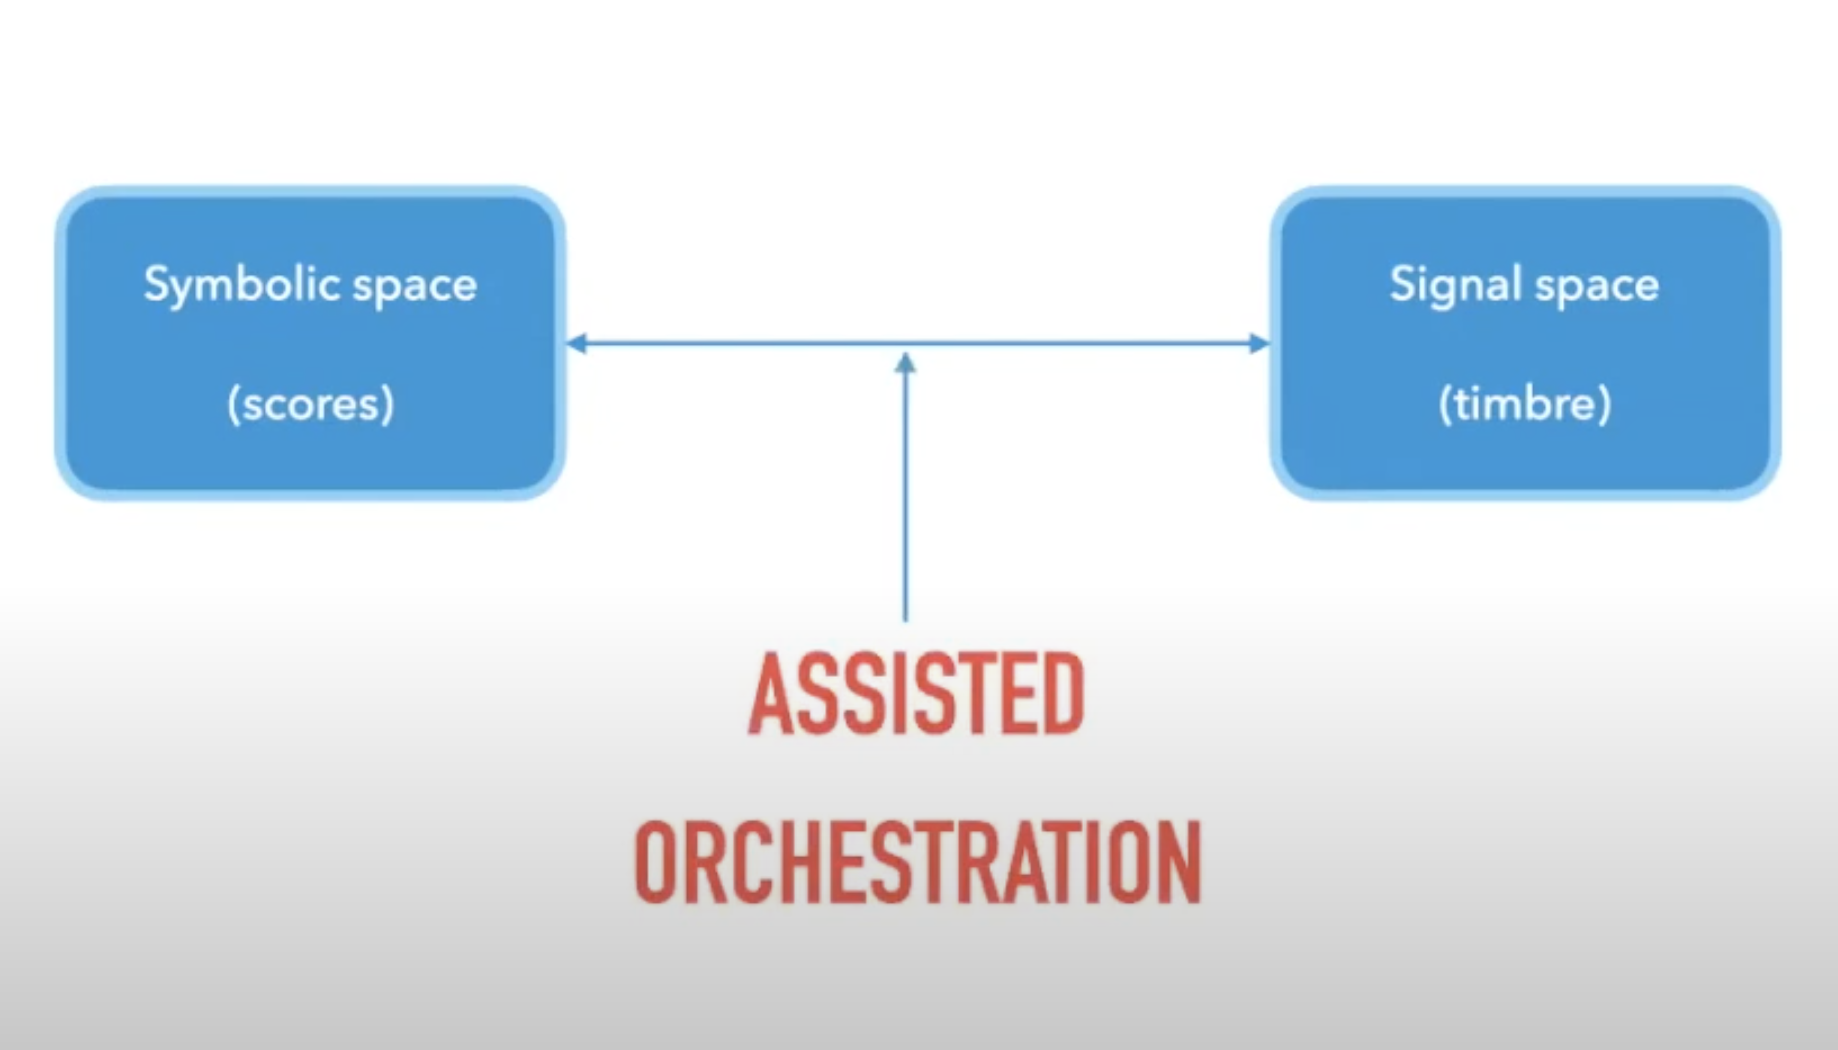
\includegraphics[scale=0.4]{assistedorch.png}
\caption{Assisted orchestration as the connection between symbolic space and signal space}
\label{figassistedorchsymb}
\end{figure}

The subject of acoustic space has been widely studied by composers in the last 20 years with composers focusing mainly on the sound itself and less on the notes themselves.  \\
\subsection{Target-based music orchestration}

\textbf{Preliminaries}

%\alex{def dynamics, playing styles..;}\\

Let us give here quick definitions of terms used later in the document. 

A \textbf{sound} is a periodic wave. It is possible to decompose this periodic wave, seen as a periodic function, using Fourier series which are a weighted sum of sinusoids.\\

The different sinusoids, being distincts from one another in terms of their frequencies, compose the harmonic series of a sound. In this series, the fundamental harmonic, i.e the harmonic with the lowest frequency and the one that is the most noticeable to a human ear, is called the first \textbf{partial} and the other frequencies, i.e the other \textbf{partials} of a sound, create the rest of the sound.\\

The first partial usually define the \textbf{pitch} of a sound, represented by notes letter from A to G$\#$.\\

The \textbf{timbre} of a sound can be seen as the quality of a sound, each instrument like a cello or a violin producing its own quality of sound. It is the timbre that gives the possibility to a human ear to identify and recognize one instrument from another. Formally, it is directly created by the harmonic series, i.e the set of partials of a sound.\\

The \textbf{amplitude} of a sound is its volume, measured in dB.\\

\begin{figure}[h!]
\centering
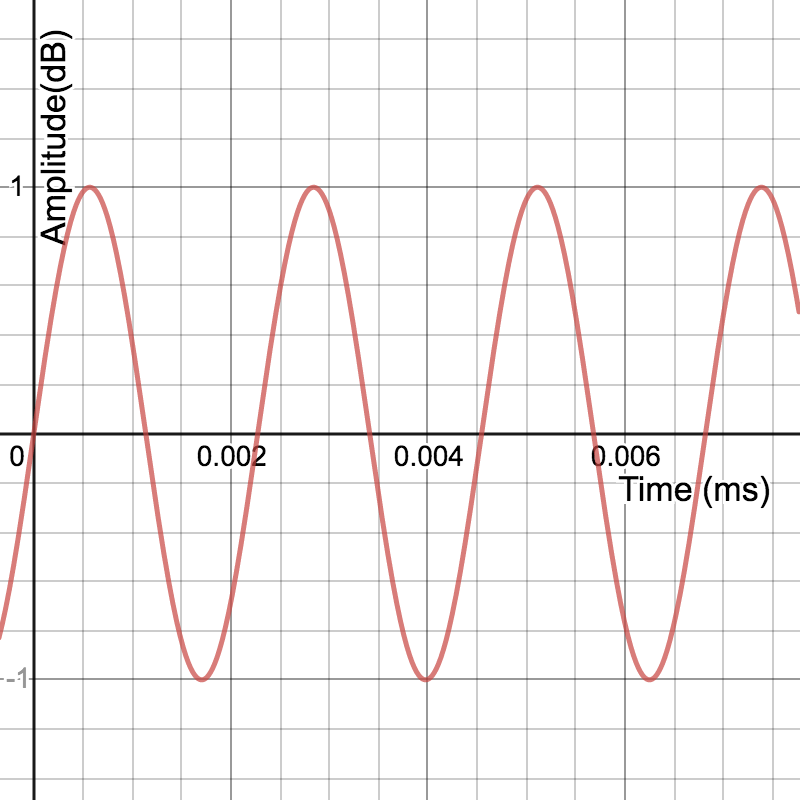
\includegraphics[scale=0.3]{A440.png}
\caption{Representation of the note A}
\label{figassistedorch}
\end{figure}

\textbf{Brief history}
Let us now present briefly some key points of the assisted orchestration history. The first well known application of assisted orchestration was a piece done by J. Harvey called \textit{Mortuos Plango, Vivos Voco (1981}) who reproduced the audio of a bell and received a warm welcome. ``It showed that IRCAM institute's apparently esoteric research program could yield music capable of appealing to a wider audience'' said Curtis Roads, a famous composer. It thus gave wider perspectives and motivations of what assisted orchestration can do. Harvey tried in this piece to transcribe the sound of the bell and retranscribe it by synthesis. The transcription was done manually at the time looking at the partials of a sound.\\
Later in 2008, in a piece called \textit{Speakings}, J. Harvey used \textit{Orchidee}, an older version of \textit{Orchidea} presented later in the chapter, in order to replicate the sound of a human voice.\\

To write a music score, a composer simply writes symbol in a music sheet. Then, the symbols are ``played'' generating sound. \\
Assisted orchestration can be seen as the other way around. Indeed, in this case, given a sound, a composer tries to find its corresponding score. This differs from music transcription, where the sound is someone playing an instrument and then one needs to find the corresponding score often using the same instrument. Indeed, in assisted orchestration the sound can be anything like bells, noise, voices$\ldots$ for which there is no corresponding score. One can say that assisted orchestration is a general case of musical transcription. \\

The assisted orchestration problem can also be seen as the problem corresponding to, given an orchestration, reproducing a target timbre within a computational context. Namely, given specific writing constraints of the composer like an orchestra with a set of chosen instruments, playing styles, dynamics$\ldots$, is it possible to be as close as possible to the target sound. \\

% Formally, this problem can be seen as a multi-objective one:
% \begin{itemize}
%     \item a combinatorial optimization problem defined on the description of the timbre
%     \item a constraint solving problem defined on the symbols of musical writing
% \end{itemize}
% This points out the connection between the symbolic space and the signal space.\\

Let us present an example in order to show the hardness of the problem.

\begin{ex}
Given a target sound, one is ask to reconstruct the sound using instruments of a restricted orchestra composed of only two instruments being able to play only two notes at a fixed single dynamic. \\
To solve this problem, one has to find the best combination of sounds, being the closest one to the target sound, among the set of possible combinations. Indeed, one can choose to take the first note on the first instrument and on the other instrument, the second note on the first instrument and on the other instrument, the first note on the first instrument and the second note on the other instrument, the first note on the second instrument and the first note on the other instrument.
For each of the four combinations, one has to compute a distance between the combination and the target sound. Under this specific set of very restricted constraints it is easy to find the best possible solution in a small amount of time. \\
\end{ex}
However, in practice the set of feasible solution is way larger: each instrument of an orchestra has the possibility to play around forty notes, several dynamics, articulations, playing styles$\ldots$. The number of different combinations in a basic setting is around $2^{30000}$ making the problem intractable. An analysis of the problem complexity will be presented later in this chapter.\\
Typical solutions to this problem are orchestral scores that include specific instruments, notes, dynamics and playing styles such that, when played, they sound perceptually similar to the target sound. In principle, to find the combination of orchestral sounds that sounds the closest to the target, it would be enough to compute all possible combinations of the sounds in the database and rank them by a distance measure with the target sound. This approach, while conceptually justified, is normally not computable given the large amount of possible combinations.\\

The intractability of the problem leads to the introduction of heuristics computing forecast. 
Indeed, the general structure of the algorithm (see \ref{fig:generalstructstat}) consists of, given:
\begin{itemize}
    \item a \textbf{target sound}
    \item a set of \textbf{symbolic constraints} i.e musical constraints
    \item a set of \textbf{sounds} in the database
    \item a \textbf{search engine} computing:
    \begin{itemize}
        \item the \textbf{feature forecast}: for each combination its feature are forecast using an heuristic
        \item the \textbf{dissimilarity measure}: measure evaluating the distance between two sounds 
    \end{itemize}
    \item the search engine then optimizes the instance and give a \textbf{score} as an output
\end{itemize}

\begin{figure}[h!]
\centering
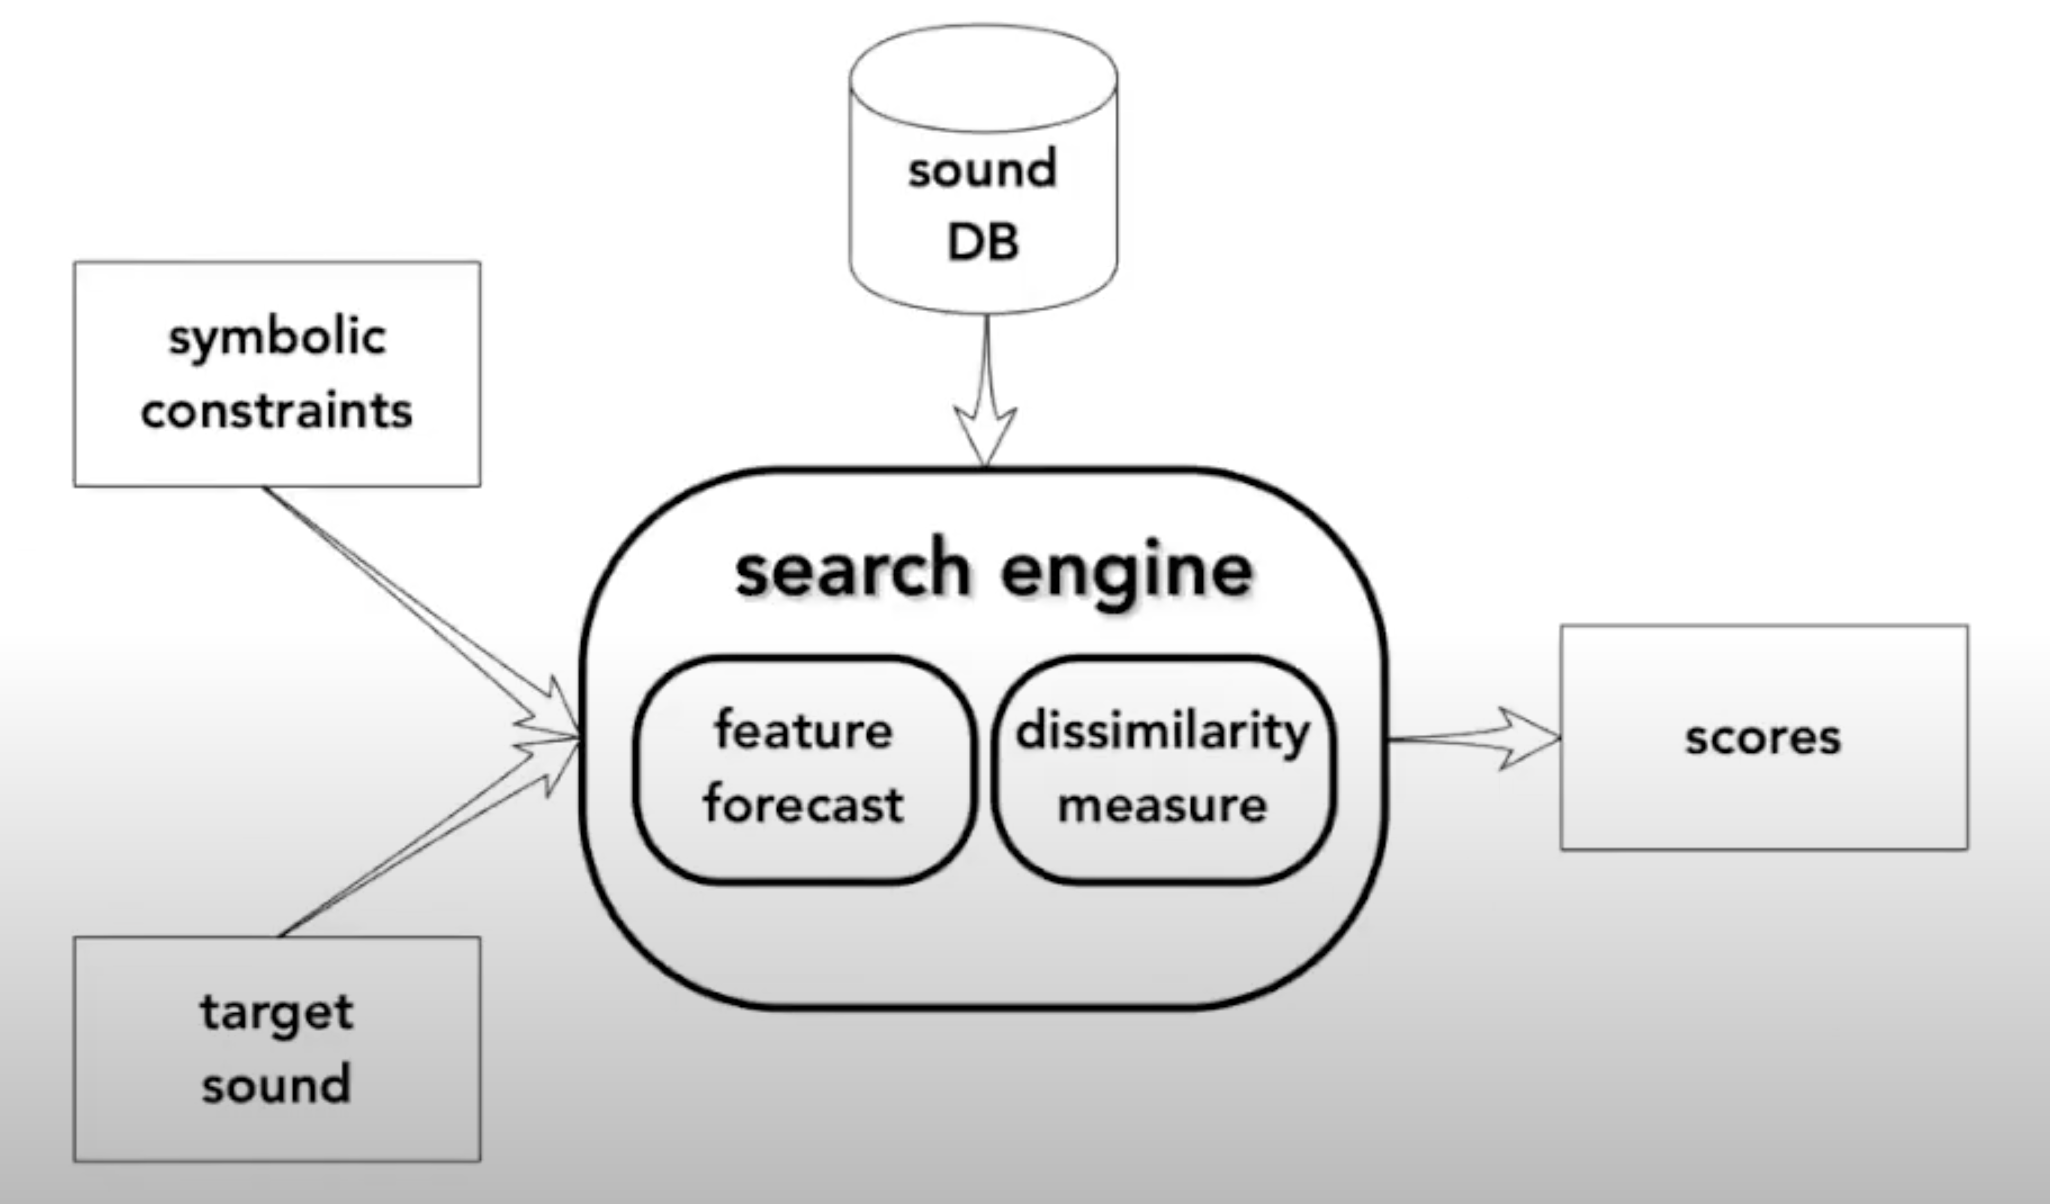
\includegraphics[scale=0.4]{generalstructstat.png}
\caption{General structure of the assisted orchestration algorithm}
\label{fig:generalstructstat}
\end{figure}

Let us say again that the outcome of an assisted orchestration algorithm is a score, i.e a set of symbols, and not sound. One can play the score using some sound database containing the instruments of the solution to be able to directly compare the solution sound to the target sound but the aim of the algorithm is to help a composer reproduce a given sound with a set of instruments.\\


Note that the choice of the dissimilarity measure and its distance is still an open question in the literature. Indeed, some hypothesis are made on the distance but up to our knowledge there is not one measure being better than the others. The hardness of this choice comes from the fact that the two compared sounds have to be close for example regarding their respective spectrum description (this notion will be defined later) but this does not necessarily imply that the two sounds will be close from the perspective of a composer, or from the human ear. 

\subsection{The search engine: features forecast and dissimilarity measure}
Let us now develop the search engine and the notions behind the feature forecast and the dissimilarity measure. \\

The sounds of the database are described by features. 
%We will develop later the different features existing in the literature, for now it is just relevant to notice that each sound is described by a chosen feature.
Each feature (a few of them exist in the literature) describes the sound with a specific metric and has a fixed number of dimensions. For example, in Figure \ref{fig:searchengine}, each sound is described by a feature of dimension $K$, i.e to each sound is associated a vector value of dimension $K$: $d_1, \ldots, d_K$ (note that in our analysis presented later in the chapter, we say that, to each sound $i$ is associated a vector value of dimension $M$: $p_{i1}, \ldots, p_{iM}$). In the first assisted orchestration algorithm that we will present, one makes a random combination between the sounds (the techniques used by the algorithm will be develop later in the chapter). Then, with the combination obtained, one needs to find the features of the combination, i.e the features of the sounds selected by the algorithm. However, in practice, it is not possible to compute the exact features of the combination, being too large and taking too much time to compute. This is where the notion of \textbf{features forecast} is introduced. Indeed, features are only predicted and their calculation themselves is a difficult problem, the features being, for most of the cases non linear features (two ways of computing the features will be presented in the chapter). \\
Once the features forecast of the combination is predicted, one needs to describe the target sound with the same features (note that here, the features of the target sound are its ``real'' features, the complexity of computing them being small because the calculation is being applied only to one sound). Only then, a distance is made, the \textbf{dissimilarity measure}, between the features of target sound and the features of combination found by the algorithm. \\

\begin{figure}[h!]
\centering
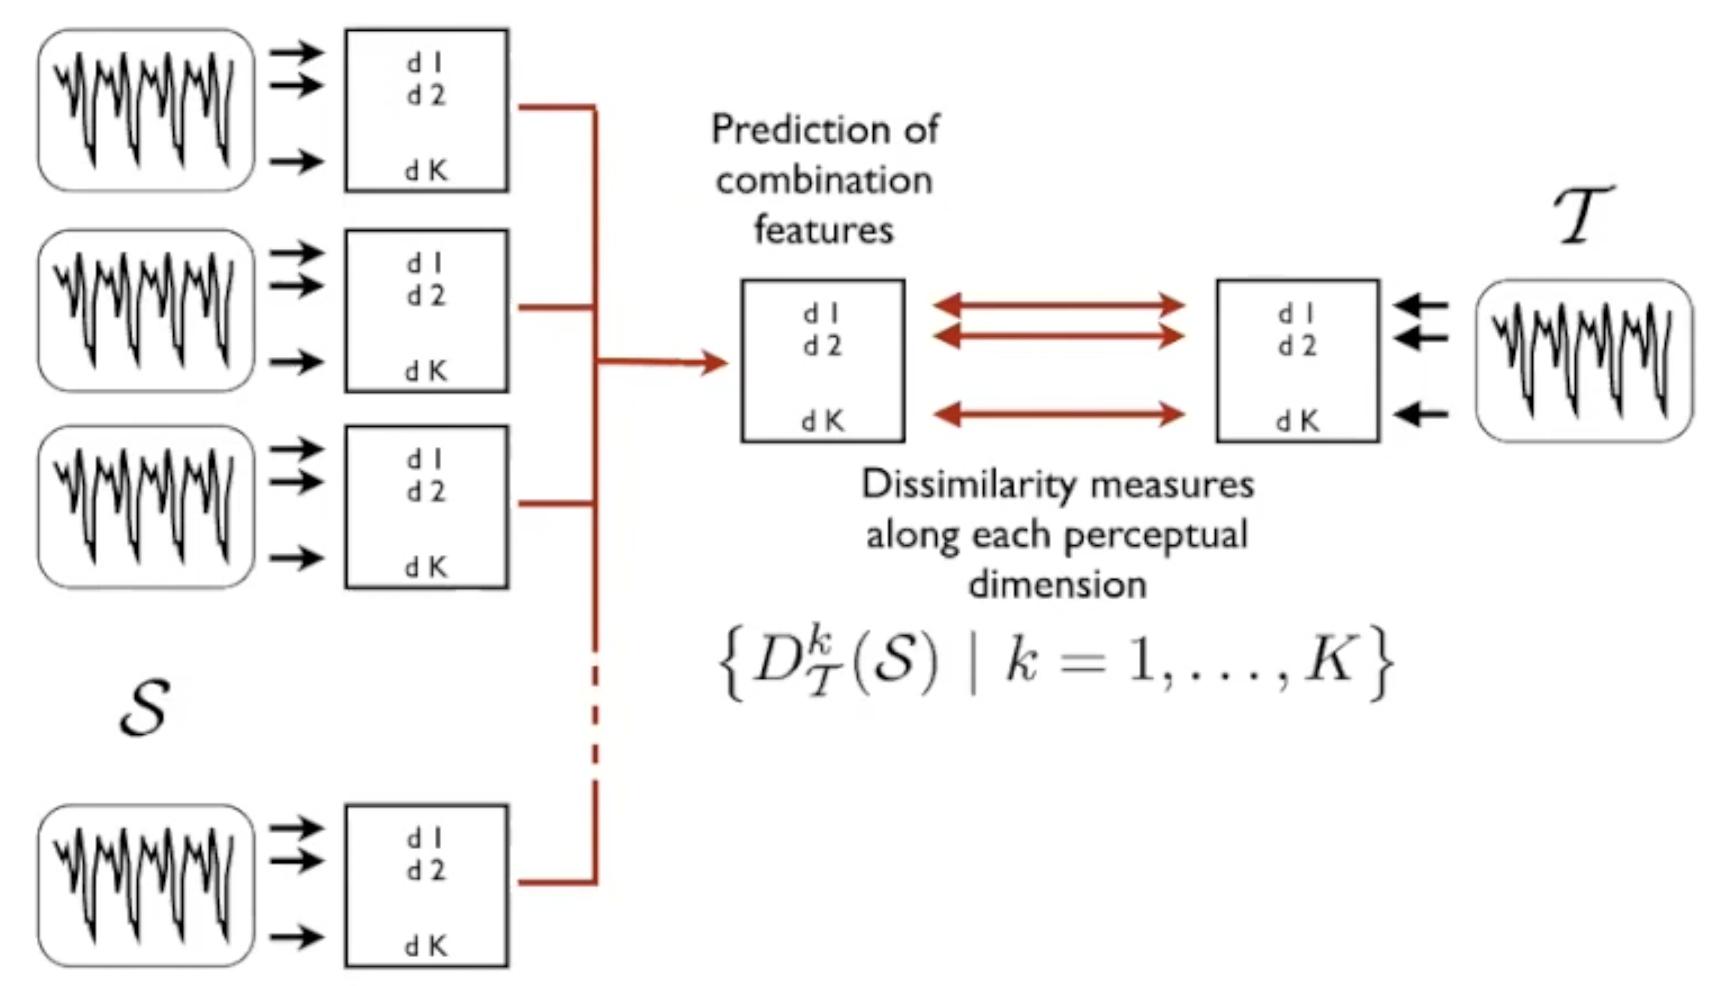
\includegraphics[scale=0.4]{searchengine.png}
\caption{The search engine}
\label{fig:searchengine}
\end{figure}

We see in Figure \ref{fig:searchengine} an illustration of the search engine, the set $\mathcal{S}$ of sounds on the left of the figure being the sounds of the database described with $K$ dimension features. A random combination of sounds is then generated and its features description predicted. We see on the right of the figure the target sound $\mathcal{T}$ described also with $K$ dimension features. The two of them are then compared using a distance, the dissimilarity measure $D^k_\mathcal{T}(\mathcal{S}) | k=1,\ldots,K$, applied on the features. The measure will be developed later in the document (note that the choice of the problem parameters notations will be different, for the sake of clarity, in our analysis presented later in this chapter with a different notation for the distance, a number of dimension $M$ and $p_{ij}$ the value of a sound $i$ in dimension $j$).\\


\section{An overview of target-based music orchestration}\label{otargorch}

In this section we will present the Target-based computer-assisted orchestration and the software called \textit{Orchidea} doing it. \\
%Therefore, not being an expert in the musical and orchestration domains, all definitions, observations and figures are directly taken from this presentation . \\ 


The main reference page is www.orch-idea.org where are presented the software, the system and the information.\\
The \textit{Orchidea} software is an assisting tool that does not orchestrate but helps the composer to orchestrate. It was developed by a few researchers including Carmine Cella, currently teaching at Berkeley university and that is accountable for the latest version of the software. He worked with IRCAM (Institut de recherche et coordination acoustique/musique), Berkeley and the HEM (Haute Ecole de musique de Geneve). \\




The approach implemented in \textit{Orchidea} works as follows and will be developed more into details in this chapter:
\begin{itemize}
	\item a target sound and a database of orchestral sounds are embedded in a high-dimensional feature space;
	\item the target sound is cut into segments that represent the temporal variations;
	\item each segment is timbrally matched against a large number of combinations of sounds of the database
	by means of a multi-stage algorithm that optimise both the features and the symbolic constraints;
	\item the best match for each segment is then connected temporally to the other best matches in order to produce a musically meaningful score.
\end{itemize}



The approach discussed above is depicted in figure \ref{fig:orchidea_overview} in the subsection presenting the \textit{Orchidea} software.

\begin{figure}[ht!]
\centering
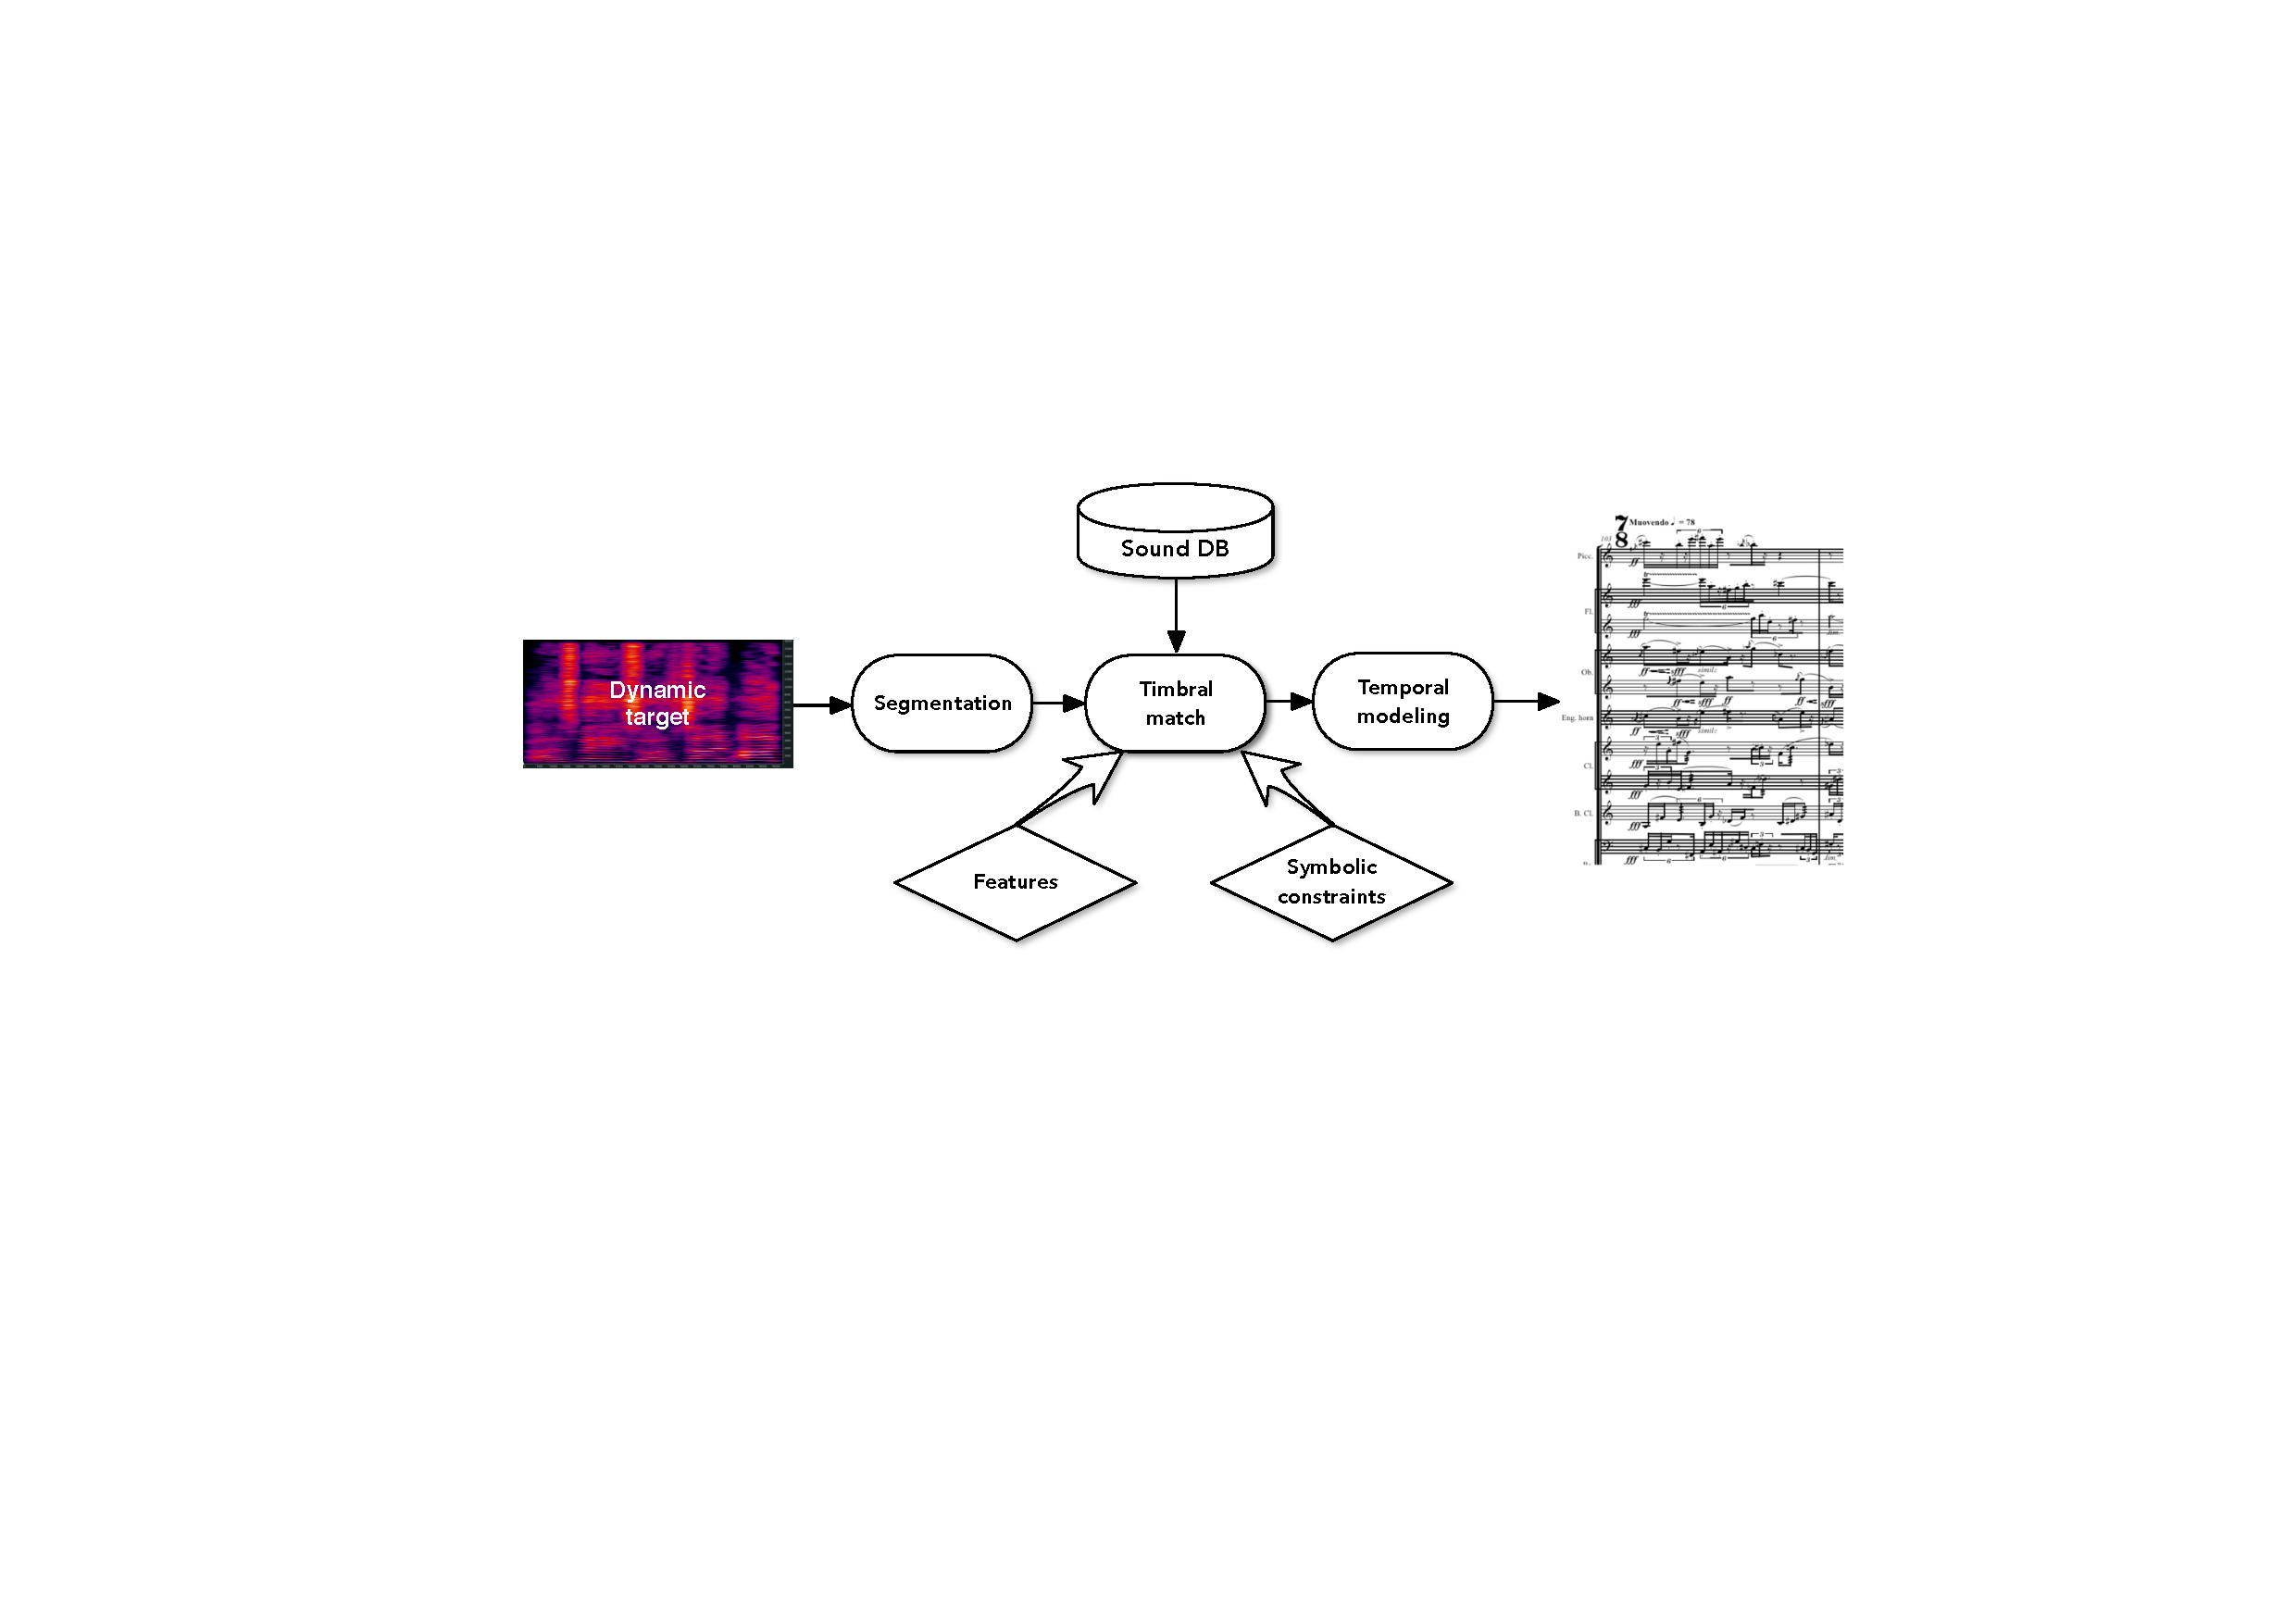
\includegraphics[scale=0.6]{Orchidea_overview.pdf}
\caption{An overview of \textit{Orchidea}, the state-of-the-art system for dynamic target-based orchestration. The three main stages of the algorithm implemented in \textit{Orchidea} are the segmentation of the target, the timbral match and the temporal modelling of the solutions.}
\label{fig:orchidea_overview}
\end{figure}




\subsection{The original software: \textit{Orchidee}}%idea behind the assisted orchestration problem}

Let us now present the idea behind the assisted orchestration software called \textit{Orchidee}.\\
Indeed, a solution to the target-based music orchestration problem proposed in \cite{carpentier2007evolutionary}, consists in using a multi-objective genetic heuristics and a constraint solver that are jointly optimized. The target sound and the sounds in the database are embedded in a low-dimensional feature space (in contrasts with the high-dimensional one for \textit{Orchidea}) and each generated combination of sounds is evaluated with a distance metric. 
This approach is solely focused on the so-called \emph{static} aspect of the problem: the target sound is considered as time-invariant and the algorithm does not consider any timbral change over time.

Let us now develop it more into details.\\
Using only a few features, the sound is embedded in a low dimension space. The selected features describing the sound of the database are called perceptual features i.e relevant for the perception features such as the pitch, the energy, the brightness, the bandwith,$\ldots$. \\

Then a multiobjective optimization algorithm is applied to the instance, minimizing jointly all the features describing the sounds with value $D^k_\mathcal{T}(\mathcal{S}) | k=1,\ldots,K$.\\
The algorithm then generates a set of solutions that can be represented as a Pareto front.\\
%\alex{mettre ref ?? DeFINIR Pareto} \\

Indeed, each solution on the Pareto front would be better according to a given feature, for example, one solution would have the best pitch, another would have the best brightness, $\ldots$.\\
This approach was very useful for the composers that could choose between the set of all the Pareto dominating solutions according to their personal listening preferences between the features. The assisted orchestration problem was implemented this way around 2007 in the \textit{Orchidee} software.\\
This approach was developed and presented in the thesis by Carpentier in 2008 (\cite{carpentier2008approche}).\\

In order to address a risk of combinatory explosion, a genetic algorithm was developed to thwart the impossibility of computing all the combinations of sounds. The genetic algorithm indeed generates a random combinations of sounds ``good enough'', i.e not optimal but close to it. \\
Let us now present informally the genetic algorithm used in the \textit{Orchidee} software. It starts with a random combinations of sounds, for example $500$ random combinations of sounds, and then the \textit{fitness} of the combination is calculated, ranking it in comparison to the target. Then, genetic transformations called crossover and mutation are applied to the best found combination of sounds. The crossover transformation takes, given two combinations, part of one combination and part of the other combination. Then, the algorithm generates a new combination of sound being a mix of the two combinations. Next, the algorithm applies a mutation on the produced combination of sounds, i.e altering the combination of sounds by a random factor. Finally, the fitness of this last combination is computed again, being able to rank again the solutions found. Then, the mutation and the crossover operations are applied again on the best found solution generating a new solution on which the \textit{fitness} is computed again. The algorithm does these series of operations over and over again until the solutions found converged, i.e the value of the solution does not change too much between two series of genetic operations. The solution found at the end is ``good enough''. To be more precise, the genetic algorithm of \textit{Orchidee} works as follows:\\

\textbf{Genetic assisted orchestration algorithm}
\begin{enumerate}
    \item Initialization:
    \begin{itemize}
        \item Generate randomly an initial combination of sounds 
        \item Compute the fitness of the combination of sounds 
    \end{itemize}
    \item While the fitness of the solution has not converged do:
    \begin{itemize}
        \item Rank the solution found and find the best combination of sounds
        \item Apply the crossover operation to the best solution found
        \item Apply the mutation operation to the best solution found
        \item Compute the fitness of the solution
    \end{itemize}
    \item Output the solution
\end{enumerate}

This algorithm was developed in 2008 and is the foundation of the current assisted orchestration tool that we are going to present now.

\subsection{\textit{Orchidea}}\label{sec:orchidea}

While the problem adressed by the \textit{Orchidee} software is an interesting problem, in practice no real sounds exhibit a time-invariant nature. As such, the computer-assisted orchestration problem can be formulated in a \emph{dynamic} manner: the parameters of the algorithm should change over time, to account to the timbral changes of the target sound.
This approach, that requires many more parameters and has a greater computational complexity, has been discussed in \cite{Cella2018},
\cite{Cella2020b} and is implemented in the \textit{Orchidea} toolbox for assisted orchestration ({www.orch-idea.org}), currently considered the state-of-the-art system for target-based computer-assisted dynamic and static orchestration.


\textit{Orchidea} is the assisted orchestration tool on which our theoretical studies presented later in the document were based on. Until \textit{Orchidea}, the assisted orchestration mainly dealt with static target sound, i.e with a single sound like a note of an instrument, a bell, $\ldots$. \textit{Orchidea} focuses on both static and dynamic/temporal target sounds. Indeed, the target sounds can now be dynamic, like a whole piece of music, a series of sounds, $\ldots$ To deal with the temporal aspect of assisted orchestration, \textit{Orchidea} introduces two new approaches in the assisted orchestration framework, a joint time-target optimization and connection models. These two approaches will be developed later in the section. \\
The implementation of \textit{Orchidea} began in 2017 and is still in development, a first public and usable version with a modular interface was presented in 2019 on the visual programming language MAX/MSP (see \ref{fig:max}) as well as a standalone application. \\

\begin{figure}[!ht]
    \centering
    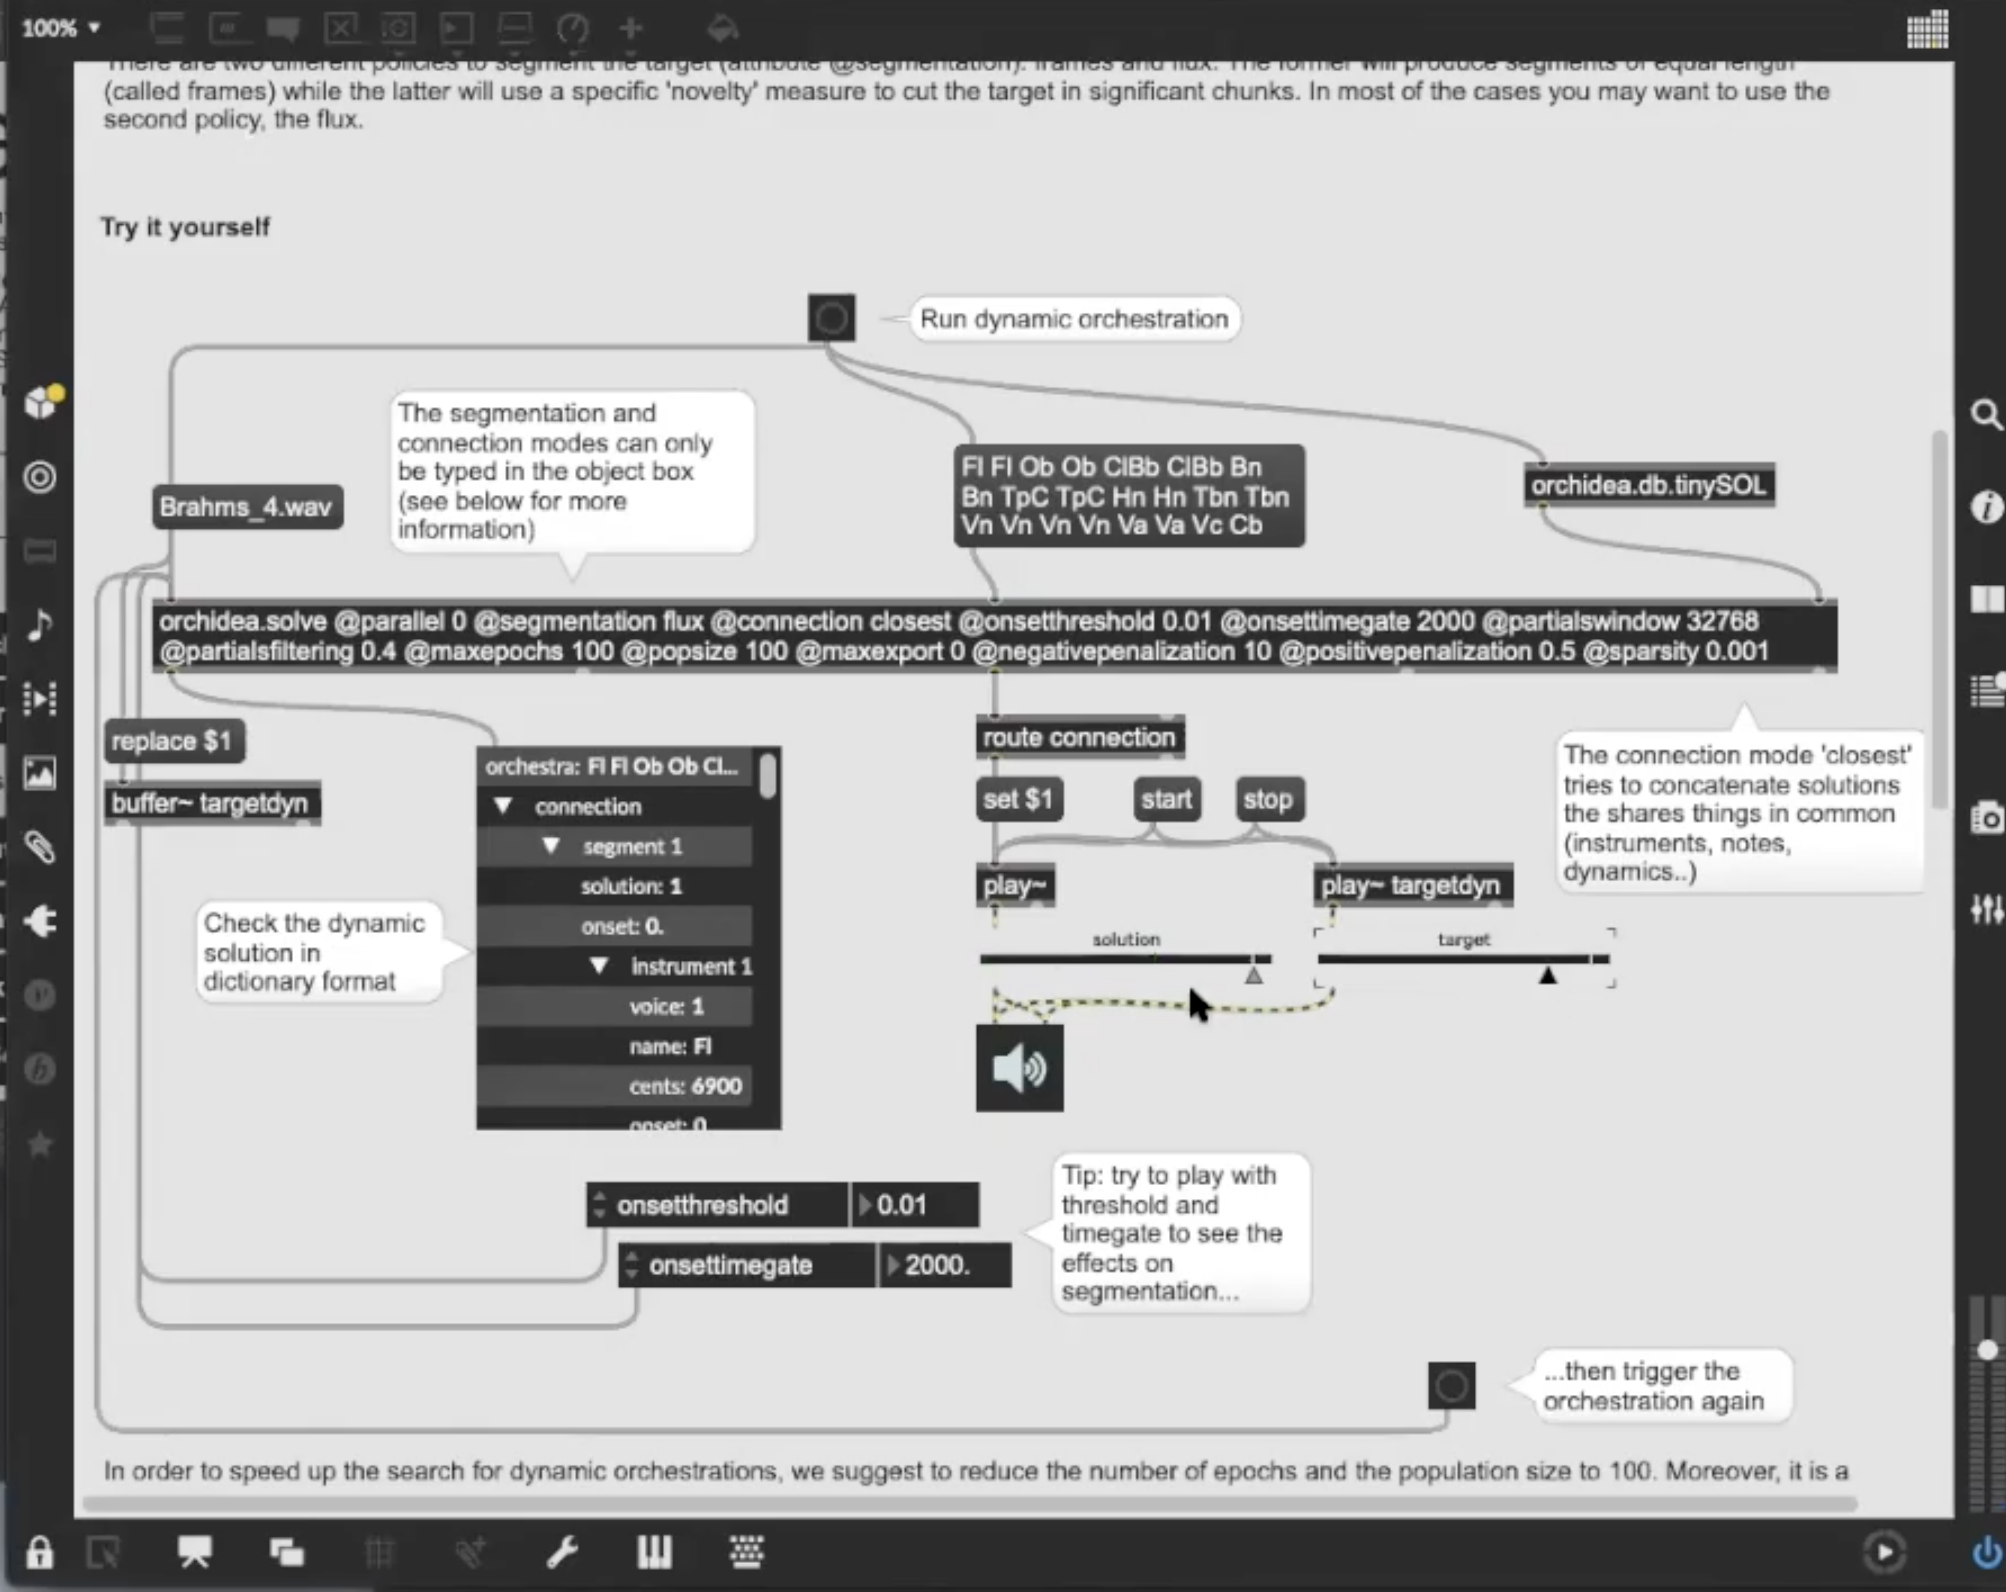
\includegraphics[scale=0.4]{maxsol.png}
    \caption{The \textit{Orchidea} software in MAX/MSP}
    \label{fig:max}
\end{figure}

The current architecture of the \textit{Orchidea} software can be described as:
\begin{itemize}
    \item an high-dimensional mono-objective optimization function with dynamic symbolic constraints. This contrasts with the previous approach that was multi-objective with  low-dimensional description. The choice of this new approach, increasing the abstraction level, was motivated by being closer to composers, to what they are looking for when they are using the assisted orchestration tool and less focused on sound analysis itself;
    \item a greedy strategy is used to generate the initial population of sounds. This contrasts also with the existing approach where random combinations were used. The greedy strategy, called stochastic pursuit strategy, finds the closest best solution and generates the initial combination of sounds;
    \item a neural network to predict the features of the sound combinations contrasting with the previous genetic approach developed in \textit{Orchidee};
    \item an asymmetric distance for the evaluation of the solutions (the dissimilarity measure). This new distance uses two new variables called positive and negative penalizations. This will developed later in the document;
    \item a joint time-frequency optimization called hysteresis of the orchestration where the solutions found on previous time steps are weighted in order to connect the solutions of the current time step with the previous ones. This will also be developed later in the document;
    \item temporal modeling graph: a representation of the dynamic orchestration problem as a graph and the introduction of the continuity model.
\end{itemize}

Let us now introduce the notion of segmentation of a dynamic sound target. Indeed, a dynamic sound target is decomposed into slices respecting the temporal variations and generates a segmentation of the target with a fixed number of time steps. To be more precise, to each time step is associated a static target sound on which calculations are applied.




% The figure \ref{fig:orchidea_overview} represents an overview of \textit{Orchidea}.\\
First, a dynamic target is segmented and decomposed into static target sounds, i.e the temporal target is cut into slices. Then, the features of sound combinations are forecast using a neural network. Next, the forecast is matched with the target sounds using the stochastic matching pursuit and the evolutionary optimization algorithms subject to a set of symbolic constraints. Finally, temporal modeling is calculated with a joint time-frequency optimization algorithm and taking into account the continuity of the solutions, i.e the continuity model. \\

\begin{figure}[ht!]
    \centering
    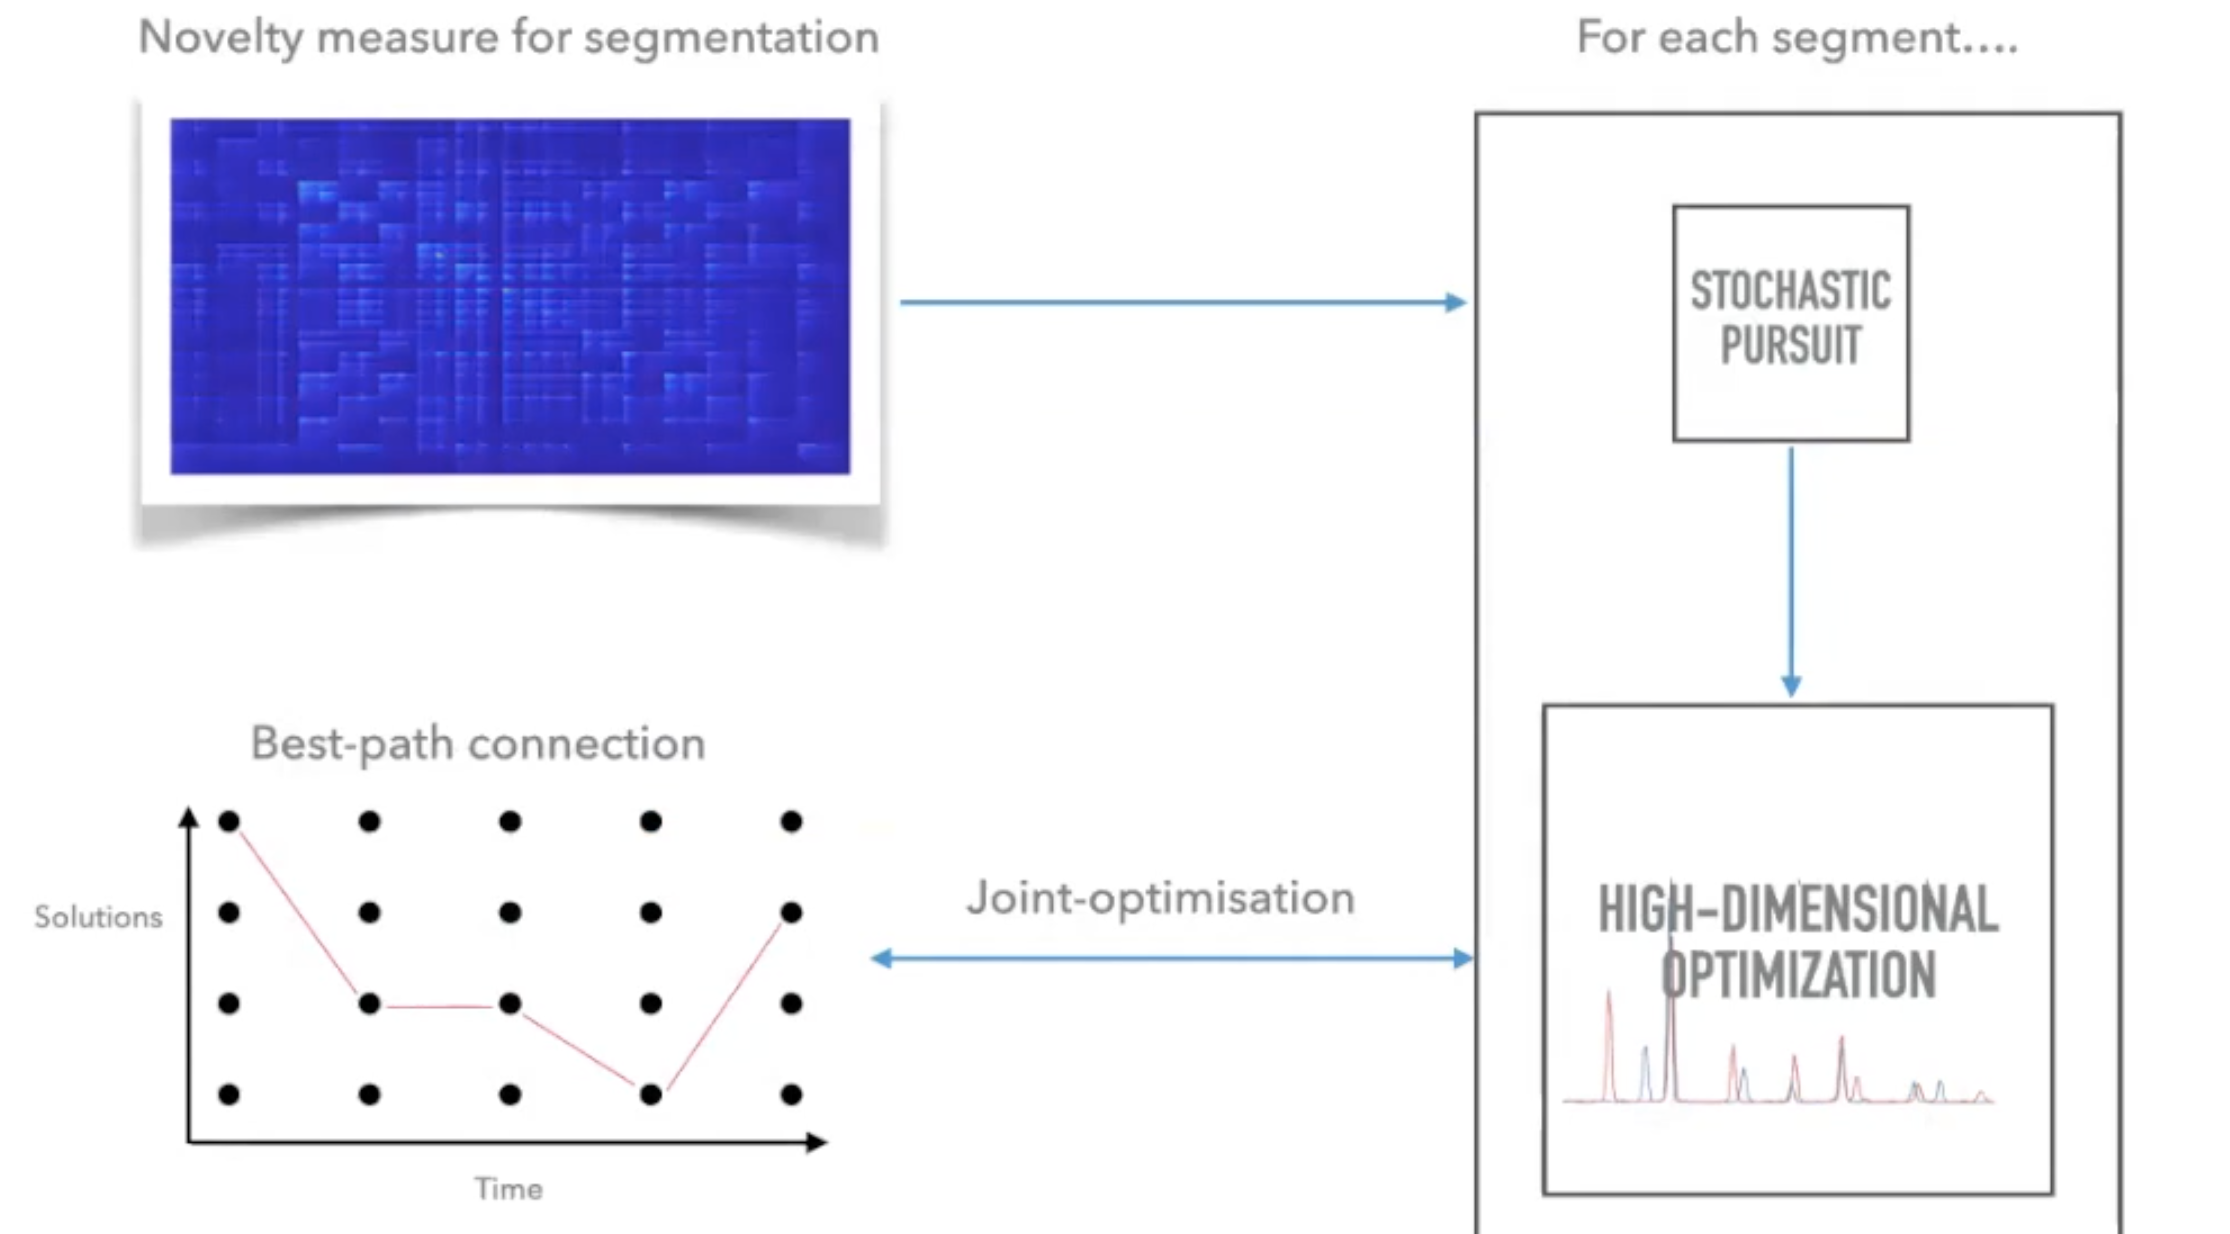
\includegraphics[scale=0.3]{tempmodel.png}
    \caption{Temporal modeling of \textit{Orchidea}}
    \label{fig:tempmodel}
\end{figure}

Figure \ref{fig:tempmodel} presents the way temporality is addressed in the \textit{Orchidea} software.
Given a temporal target sound, a segmentation is generated according to a novelty measure, i.e each time the sound is ``new'' a new slice/time step is generated. On each time step/segment generated is applied stochastic pursuit and high-dimensional optimization. All solutions are represented as a graph (we use the same technique in the next chapter, the construction of the graph will be detailed then) and joint-optimization is applied on both paths of the graph and the target of the next time step in the instance of dynamic orchestration. Indeed, a best-path connection is done connecting the different segment/time steps of the dynamic orchestration in order to both minimize the distance to the target sound and the changes in the solution between two consecutive time temps, i.e for the solution to be as stable as possible across the time horizon. This stability echoes the multistage framework.\\

The stability of a solution in a dynamic orchestration problem is evaluated using a so called continuity model, limiting as much as possible the movements in the solution. This means that when a sound is taken it is best to keep it at the next time step. Indeed, if a sound is kept for two consecutive time steps, the solution will ``connect'' the different time steps together. This connection implies better results acoustically as the sound generated by the instrument will be continuous. (See figure \ref{fig:contmodel}).

\begin{figure}[ht!]
    \centering
    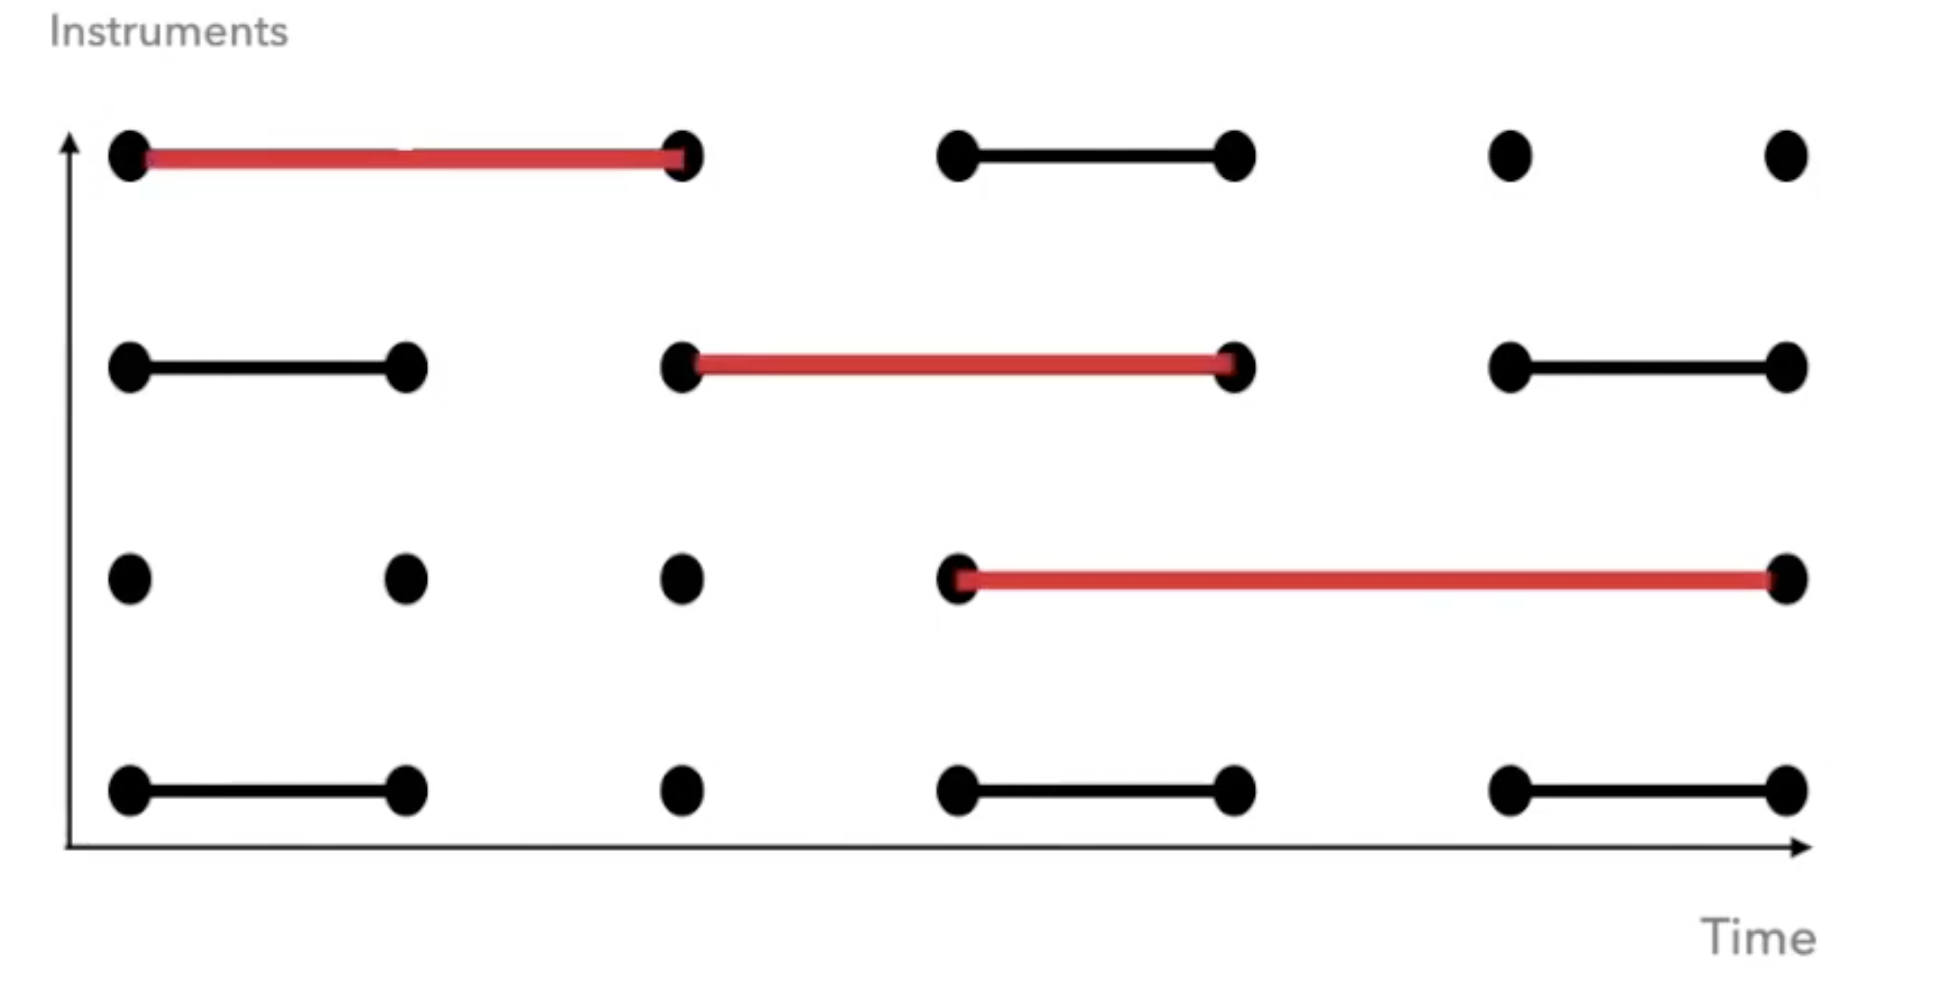
\includegraphics[scale=0.35]{contmodel.png}
    \caption{Illustration of the continuity model}
    \label{fig:contmodel}
\end{figure}

\section{Target-based computer-assisted orchestration: a theoretical analysis}\label{sec:theor}
\sectionmark{Theoretical analysis}

We presented in the previous section the musical problem {\sc Target-based computer-assisted orchestration} and its applications. Now we will address the problem with a theoretical point of view, being closely related to the multistage framework and compare results obtained with an ILP formulation to the \textit{Orchidea} ones.

\subsection{Problems definition and results}\label{sec:def}
%\subsection{Problems definition}

%As mentioned in introduction, the goal is to select sounds in a database in order to reproduce as well as possible a given sound or melody ...

We now formally define the target-based orchestration problems we focus on in this chapter. 

{\bf Sounds.} We have a set $N=\{s_1,s_2,\dots,s_n\}$ of $n$ sounds, corresponding to the database of sound samples. Each sound is produced by  an instrument. Formally, $N$ is partitioned into $N_1,\dots,N_Z$ where $Z$ is the number of instruments. Besides its instrument, each sound $s_i$ is characterized by its values on several dimensions (feature space): formally, to $s_i$ are associated $M$ nonnegative values $p_{ij},j=1,\dots,M$, where $M$ is the number of dimensions.

We also have  target sound $G$, typically not in the database $N$. As any sound, $G$ has a description in the feature space, i.e., it has a value $G_j$ on each dimension $j=1,\dots,M$.

{\bf Subset of sounds.} The goal of the problem is to choose a subset of sounds to be played by the orchestra to reproduce in the best possible way a given target. To evaluate the quality of such a subset of sounds, we first give its value in the feature space (dimensions), and then define how to evaluate the quality of this subset with respect to a target. 

Let $S\subset N$ denotes a non empty subset of sounds. The value of $S$ on dimension $j$ is the average value of each sound in $S$ on this dimension. Formally, writing $p_j(S)=\sum_{s_i\in S}p_{ij}$, the value of $S$ on dimension $j$ is $\frac{p_j(S)}{|S|}$. 

{\bf Distances.} As explained before the value of (a subset of) sounds on the dimensions allows to define a distance between them, measuring how different they are (also called before the dissimilarity measure). Formally, let $S,S'$ be two non empty subset of sounds. The {\it distance} between these two subsets is defined as $$d(S,S')=\sum_{j=1}^M \left| \frac{p_j(S)}{|S|} - \frac{p_j(S')}{|S'|}\right|$$
Note that $d(S,S')=0$ if and only if $S$ and $S'$ have the same value on each dimension.

{\bf Orchestration constraints.} As explained in Section~\ref{sec:tbmo}, in the target-based orchestration problem, we want to reproduce with an orchestra a given target sound. Then, the sounds we select in the database (to be played by the orchestra) must respect some constraints based on the orchestra composition (if there are two transverse flute, then we cannot select more than two sounds played by a transverse flute). Formally, we can have:
\begin{itemize}
    \item For each instrument $z$, a constraint $L_z$ on the number of selected sounds played by instrument $z$ that can be selected. The constraint is hence $|S\cap N_z|\leq L_z$.
    \item A constraint on the total number of chosen sounds: $|S|\leq L$ (this could be the total number of instruments, or a more restrictive constraint imposed by a composer).
\end{itemize}

\noindent {\bf Static target-based orchestration problem}

Now we are able to define the static target-based orchestration problem \stat.

\begin{definition}
In the problem \stat, we are given a set $N$ of sounds, a target sound $G$, and a set of orchestration constraints. The goal is to find a nonempty set $S$ of sounds which minimizes $d(S,G)$, while fulfilling the orchestration constraints.
\end{definition}

In the theoretical analysis of \stat, we will first focus on a simple version of the problem, where there is one instrument, no orchestration constraints, and only one dimension. We will denote this problem as \statoned.\\  

\noindent {\bf Dynamic target-based orchestration problem.}

Now let us look at the Dynamic Target-based Orchestration Problem \dyn. Think for instance that we want to reproduce a human pronouncing a sentence (the target). As explained in Section~\ref{otargorch}, the target is first cut into segments, say $T$ segments, and each segment $t$ corresponds to a target sound $G^t$. The sentence can be for instance cut into syllables, giving a sequence of syllables/tagets $G^t$. 

Then, we shall select in each time step (segment) $t$ a subset of sounds $S_t\subset N$ to reproduce $G^t$. The distance $d(S_t,G^t)$, measuring how far $S_t$ is from $G_t$, should be minimized. Besides, from musical perspective, it is also interesting to select subset of sounds that do not differ two much in consecutive time steps, i.e., $d(S_t,S_{t+1})$ should be also small. Typically, if selected subsets are similar, use the same instruments and/or notes, the solution sounds more melodious (see Section \ref{otargorch}). 

In the model we consider, we linearly aggregate these distances, and get the following problem.


\begin{definition}
In the problem \dyn we are given a set $N$ of sounds, a set of orchestration constraints, a time horizon $T \in \mathbb{N}^*$, a target $G^t$ for each $t\in \{1,\dots,T\}$, and a penalty $C_t\geq 0$ for each $t\in \{1,\dots,T\}$.

We are asked to select $T$ subsets of sounds $S_{1},\dots,S_T$, such as each $S_t$ fulfills the orchestration constraints. The goal is to minimize 
$$f(S_1,\dots,S_T)=\sum_{t=1}^T d(S_t,G^t)+\sum_{t=1}^{T-1} C_t d(S_t,S_{t+1})$$

\end{definition}
Note that the set of sounds $N$, the value $p_{ij}$ of sounds on dimensions, and the orchestration constraints are static (do not evolve during the time horizon). 

In this objective function $f$, the first part measures the (average) distance of subset $S_t$ with respect to target $G_t$, we will call it {\it orchestration cost}. The second part measures  the cost from moving from subset $S_t$ to subset $S_{t+1}$, we will refer to it as {\it transition cost}. Coefficients $C_t$ allow to balance between these two costs.

\subsection{Contributions and organization of the chapter}

The main contribution of this chapter is a theoretical analysis of algorithmic properties of \stat and \dyn. We first focus on the computational complexity of the problems, both in the static case and in the dynamic case. We show that the static problem \stat is \textbf{NP}-hard, even in the very restricted case of \statoned (with only one dimension, one instrument and no constraint). 
We then show that \stat is solvable in pseudo-polynomial time (when the number of dimensions is fixed), by a dynamic programming (DP) procedure. Combining this procedure with a shortest path representation capturing temporality, we show that the pseudo-polynomiality result extends to the dynamic case. We also propose approximation algorithms for both problems based on rounding techniques from the DP procedures. Table~\ref{table:results} sums up the results we obtain.
\begin{figure}
\begin{tabular}{r||c|l|l}
     &   & Pseudo-polynomial &Polynomial time \\
        Problem  & Complexity  & exact algorithm &   approximation algorithm\\
     \hline \hline
     \statoned &  NP-hard & $O(n^3p_{max})$ & $OPT+\epsilon p_{max}$ in time $O(n^3/\epsilon)$ \\ \hline
          \stat &  NP-hard & $O(L^2n^{M+1}p_{max}^M)$ & $OPT+\epsilon p_{max}$ \\ 
                     &   &  &  in time $O(L^2n(nM/\epsilon)^M)$ \\ \hline
               \dynoned &  NP-hard & $O(n^3p_{max}+Tn^2p_{max}^2)$ & $OPT+\epsilon p_{max}(1+C_{max})$  \\   &  &  &  in time $O(Tn^3/\epsilon+T^3n^2/\epsilon^2)$ \\
               \hline
     \dyn &  NP-hard & $O(TL^2(np_{max})^{2M})$ & $OPT+\epsilon p_{max}(1+C_{max})$ \\ 
           &   &  & in time $O(TL^2(2nMT/\epsilon)^{2M})$ \\ \hline
\end{tabular}
\caption{Summary of results. $p_{max}=\max_{i,j} p_{ij}$ and $C_{max}=\max_{t}C_t$. $OPT$ denotes the optimal value (so error are additive in the last column).}\label{table:results}
\end{figure}

We also perform some experiments to generate orchestrations on specific targets. We evaluate our results both in a qualitative and a quantitative manner. 
The qualitative evaluation is performed by acoustic inspection of the solution and direct comparison with the solutions of the same target generated by \textit{Orchidea}. The quantitative evaluation uses the objective function of the considered model to compare solutions.

The remainder of the chapter is organized as follows. In Section~\ref{sec:1dnoc} we focus on the restricted static problem \statoned. We tackle the general static problem \stat in Section~\ref{sec:static}, and the dynamic problems \dyn in Section~\ref{sec:dyn}. Experimental results are given in Section~\ref{sec:expe}. 


\subsection{Related works in the {\sc multistage} framework}

As explained in Section~\ref{sec:def}, in the problem with temporality \dyn, we build a sequence of subset sounds $S_1,\dots,S_T$, which induces two costs: the orchestration cost $\sum_t d(S_t,G^t)$, which measures how close we are from the target, and the transition cost $\sum_t d(S_t,S_{t+1})$ which should be minimize from an acoustic viewpoint to get solution sequences that can be connected in a melodious way.

This situation, where we have a time horizon, a solution sequence to build, and an objective function mixing quality of individual solutions and transition cost corresponds to the multistage framework studied in the thesis.





\section{\statoned: complexity and approximation}\label{sec:1dnoc}

In this section, we focus extensively on the problem \statoned, where there is one instrument, no orchestration constraint, and only one dimension. Basically, each sound $s_i$ is characterized by one value $p_i\geq 0$. 

We first show that even this very restricted case of the orchestration problem is already \textbf{NP}-hard. Let us consider the decision version of this problem, {\sc Decision} \statoned, where we are given $K\geq 0$ and we are asked if there is a feasible solution of value at most $K$. 

%For readability, we will use the Garey and Johnson \cite{gj} definition framework, with problems in their decision versions.  


%\begin{definition} {\sc Orchestration 1DNOC}\\
%INSTANCE: Finite set $N$ of sounds, value $p_j \in \mathbb{Z}$ for each $j \in N$, a target $G \in \mathbb{Z}$, $K \in \mathbb{R}$.\\
%QUESTION: Is there a non empty subset $S' \subseteq N$ such that     $\left|\frac{p(S')}{|S'|} - G \right| \leq K$, with $p(S') = \sum_{i \in S'} p_i$
%\end{definition}

We will prove the \textbf{NP}-hardness by a reduction from the {\sc Equipartition} problem,  known to be \textbf{NP}-complete \cite{gj}:

\begin{definition} {\sc{Equipartition} }:\\
INSTANCE: Finite set $A$ of $q$ elements and a size $v(a) \in \mathbb{N_+^*}$ for each $a \in A$.\\
QUESTION: Is there a subset $A' \subseteq A$ of size $q/2$ such that $\sum_{a \in A'}v(a)=\frac{B}{2}$, with $B=\sum_{a \in A }v(a)$.
\end{definition}
Note that $q$ and $B$ are assumed to be even. 


\begin{theorem}\label{theo:nphardd}
$\text{\sc{Decision} \statoned}$ is \textbf{NP}-Complete, even with $K=0$.
\end{theorem}

\begin{proof}
The problem is obviously in \textbf{NP}. 

Given an instance of {\sc Equipartition} on the set $A=\{a_1,\dots,a_q\}$ with $q=2p$ elements with $B=\sum_{i=1}^q v(a_i)$, we build the following instance $I'$ of \statoned:
\begin{itemize}
\item There is a set $N=\{s_0,\dots,s_q\}$ of $q+1$ sounds: each element $a_i$ ($i\geq 1$) corresponds to one sound $s_i$, with value $p_i=v(a_i)$. $s_0$ has a large value
$M=B(q+2)$. 
\item The target is $G= \frac{M+B/2}{p+1}$, and $K=0$. 
\end{itemize}

Note that if $G$ is not integer, we can multiply the value of each sound by $p+1$ and get an equivalent instance with an integer target.

With $K=0$, the problem is equivalent to finding a subset $S \subseteq N$ s.t $ \frac{p(S)}{|S|} = G$. 

Suppose that there is a set $A'$ of size $p=q/2$ of sum $B/2$. Then the corresponding set of $p$ sounds, plus $s_0$, is a set $S$ of $p+1$ sounds, with $p(S)=M+B/2$, so  $\frac{p(S)}{|S|}=\frac{M+B/2}{p+1}=G$.

Conversely, suppose that there is a nonempty  set $S$ of sounds of average value $G$. First, notice that $S$ necessarily contains $s_0$, otherwise  $p(S)\leq B$, and $p(S)/|S|\leq B$, while $B<G$ (as $M>B(p+1)$).

Then, $S=s_0\cup S'$. We show that $|S'|=p$:
\begin{itemize}
    \item Suppose first that $|S'|\geq p+1$. Then $\frac{p(S)}{|S|}\leq \frac{M+B}{p+2}$. But with the choice of $M$, $\frac{M+B}{p+2}<\frac{M+B/2}{p+1}=G$, contradiction.
    \item If $|S'|\leq p-1$, then $\frac{p(S)}{|S|}\geq \frac{M}{p}$. But with the choice of $M$, $\frac{M}{p}>\frac{M+B/2}{p+1}=G$, contradiction.
\end{itemize}
Then $|S'|=p$, and $\frac{M+p(S')}{1+p}=G=\frac{M+B/2}{1+p}$, so $p(S')=B/2$. The corresponding set $A'$ of $p$ elements shows that the answer of the equipartition instance is yes.
\end{proof}
%The hardness result for the {\sc Static 1DNOC} problem immediately transfers to all the other versions of the {\sc orchestration} problem.

We now show that \statoned is solvable in pseudo-polynomial time, using dynamic programming. 

%\subsection{A pseudo polynomial algorithm to solve the {\sc Orchestration1DNOC} problem}

%The {\sc Orchestration} problem can be solved in pseudo polynomial time using dynamic programming. Let us first focus again on the simplified version of the problem, the \text{\sc{Orchestration 1DNOC}} problem. \\

\begin{theorem}
\statoned is solvable in time $O(n^3p_{max})$ with $n$ the number of sounds, $p_{max}$ the maximum value of a sound in $N$.
\end{theorem}
\begin{proof}

To solve the problem, we build  a truth table {\sc Tab} such that $\text{\sc{Tab}}(i,j,k) = true$ if and only if there exists a subset of the first $i$ sounds that sums to $j$ with exactly $k$ sounds (i.e of size $k$). ${\sc TAB}$ is defined for $i=1,\ldots, n$, $j=0,\ldots,\sum_{i=1}^n p_i$, and $\ k=0,\ldots,n$. 

Note that as $\sum_{i=1}^n p_i\leq np_{max}$, the size of the table is $O(n^3P_{max})$. 


We initialize {\sc Tab} when $i=1$ or $j=0$ or $k=0$, using the following four different cases: 
\begin{itemize}
		\item $TAB(i,0,0)=true$ for all $i \in \{1,\ldots,n\} $
	\item $TAB(i,0,k)=false$ for all $i \in \{1,\ldots,n\}$, all  $k \in \{ 1,\ldots,n\}$.
\item $TAB(i,j,0)=false$  for all $i \in \{1,\ldots,n\}$, all $j>0$.
	\item If $j\geq 1$ and $k\geq 1$, $TAB(1,j,k)=true$ if $j=p_1$ and $k=1$, $ false$ otherwise.
\end{itemize}

Then, for $i\geq 2$, $j\geq 1$ and $k\geq 1$ we compute $TAB(i,j,k)$ using the recursion:

 \[  \left \{  TAB(i,j,k)=
\begin{tabular}{cccc}
%$ true$  &&& if $j =0 \text{ and } k=0$\\
%$ false $&&&if $i =0 $\\
$TAB(i-1,j,k) \  ||\  TAB(i-1,j-p_i,k-1)$ &&&if $p_i \leq j$ \\
$TAB(i-1,j,k)$&&&otherwise\\

\end{tabular} 
\right.
\]

Indeed, to get a sum of $j$ with exactly $k$ sounds, we can either take the sound $s_i$ ($TAB(i-1,j-p_i,k-1)$) if $p_i\leq j$, or not take $s_i$ ($TAB(i-1,j,k)$).

Once all the {\sc Tab} is filled with respect to the previous rules, by simply browsing through the {\sc Tab}, and finding the cell where $|\frac{j}{k}-G|$ is minimal, we get the value of the solution. Then a standard backward procedure allows to recover the solution. As each cell is filled in constant time,
the overall complexity of $O(n^3p_{max})$.
\end{proof}


Now, we consider approximation algorithms.
 The problem consisting of knowing whether the optimal value is 0 or not is \textbf{NP}-hard (Theorem~\ref{theo:nphardd}). Thus it is not possible to get any $c$-approximation polynomial time algorithm, as any such algorithm allows to detect when the optimal value is 0 or not. Thus, an additive term is mandatory in the approximation result. Here, we show that by standard rounding technique, one can use the previous dynamic algorithm to get a polytime algorithm with only {\it additive} error - and no multiplicative error. More precisely, we have the following result (where {\sc OPT} is the optimal value and $p_{max}=\max p_i$).

\begin{theorem}\label{th:approx1d}
For any $\epsilon>0$, \statoned admits an algorithm which outputs a solution of value at most ${\sc OPT}+\epsilon p_{max}$ in time $O(\frac{n^3}{\epsilon})$.
\end{theorem}

\begin{proof}
Let $\epsilon>0$. Given an instance $I$ of \statoned, we construct an instance $I'$ of the same problem by rounding the $p_i$:  for all sound $s_i$ in $N$, $p_i'= \lfloor \frac{p_i }{\lambda} \rfloor$, where $\lambda=\frac{p_{max} \epsilon}{2}$. We also round the target: $G' =\frac{G}{\lambda}$. The algorithm simply computes an optimal solution $S'$ on $I'$ using the dynamic programming algorithm and outputs it. Note that the complexity of the algorithm is $O(n^3p'_{max})$, ie $O(n^3p_{max}/\lambda)=n^3/\epsilon)$ as claimed.

Let $S^*$ be an optimal solution for the original instance $I$. The remainder of the proof is to show that \begin{equation}\label{eqth3}
d(S',G)\leq d(S^*,G)+2\lambda=d(S^*,G)+\epsilon p_{max}
\end{equation}  


For any subset of sounds $S$, let $m(S) = \frac{p(S)}{|S|}$ and $m'(S) = \frac{\sum_{i \in S} p_i'}{|S|}$. From the inequality $\frac{p_i}{\lambda} \geq \lfloor \frac{p_i}{\lambda} \rfloor \geq \frac{p_i}{\lambda} -1$ we get
$\frac{m(S)}{\lambda} \geq m'(S) \geq \frac{m(S)}{\lambda} -1 $. From this, we immediately deduce:
\begin{eqnarray}
m(S) &\geq & \lambda m'(S) \geq m(S) - \lambda\\
\lambda m'(S) & \leq & m(S) \leq \lambda m'(S) + \lambda
\end{eqnarray}

Now, let us look at $d(S,G)=|m(S)-G|$:
\begin{itemize}
\item if $m(S)-G \geq 0$ then $|m(S)-G| = m(S)-G \leq \lambda m'(S)+\lambda -G = \lambda (m'(S)-\frac{G}{\lambda})+\lambda$
\item  if $m(S)-G < 0$ then
 $|m(S)-G| = G-m(S) \leq G- \lambda m'(S) = \lambda (\frac{G}{\lambda} -m'(S))$.
\end{itemize}
Then, in both cases we have:
\begin{equation}\label{eq2}
|m(S)-G| \leq \lambda \left|m'(S) - \frac{G}{\lambda}\right| + \lambda
\end{equation}

Regarding $|m'(S)-G'|$, we get:
	\begin{itemize}
		\item if $m'(S)-\frac{G}{\lambda} >0$ then  $|m'(S)-\frac{G}{\lambda}| = m'(S)-\frac{G}{\lambda} = \frac{\lambda m'(S) -G}{\lambda} \leq \frac{m(S)-G}{\lambda}$.
		\item if $m'(S)-\frac{G}{\lambda} <0$ then $|m'(S)-\frac{G}{\lambda}| = \frac{G}{\lambda} - m'(S) \leq \frac{G}{\lambda} - (\frac{m(S)}{\lambda}-1) = \frac{G-m(S)}{\lambda} +1$
	\end{itemize}
Then, we have:  
\begin{equation}\label{eq3}
|m'(S)-\frac{G}{\lambda}| \leq \frac{|m(S)-G|}{\lambda} +1
\end{equation}

Thus, using equations~(\ref{eq2}) and~(\ref{eq3}) we can bound the loss incurred by the scaling technique when considering $S'$ as a solution of the initial distance:
\begin{eqnarray}
|m(S')-G|-|m(S^*)-G| & \leq & \lambda \left|m'(S') - \frac{G}{\lambda}\right| -  \lambda \left|m'(S^*)-\frac{G}{\lambda}\right|  + 2\lambda \\
& \leq  & \lambda (\left|m'(S') - \frac{G}{\lambda}\right| - \left|m'(S^*)-\frac{G}{\lambda}\right|) + 2\lambda %\label{eq:bound}
\end{eqnarray}

By optimality of $S'$ on $I'$, we have
$|m'(S') - \frac{G}{\lambda}| - |m'(S^*)-\frac{G}{\lambda}| \leq 0$. 

Thus we get $|m(S')-G|-|m(S^*)-G| \leq 2\lambda$, ie, Equation~(\ref{eqth3}).
\end{proof}



\section{The static target-based orchestration problem}\label{sec:static}

We now consider the general static orchestration problem \stat. We recall that, with respect to \statoned, in \stat:
\begin{itemize}
    \item Each sound $s_i$ has $M$ evaluations $p_{ij},j=1,\dots,M$. We will denote $\vec{p_i}=(p_{i1},\dots,p_{iM})$ the vector of evaluations of sound $s_i$.
    \item The set $N$ of sounds is partitioned into $Z$ sets $N_z,z=1,\dots$. $N_z$, of size $n_z$, is the set of sounds played with a given instrument. The number of sounds chosen in $N_z$ cannot exceed $L_z$, while the global number of sounds cannot exceed $L$. 
\end{itemize}

\stat is of course \textbf{NP}-hard, as it generalizes \statoned. In this section, we show how the dynamic programming algorithm and the approximation algorithm generalizes to \stat. 
We first start by the dynamic programming algorithm, showing that \stat remains pseudo-polynomial when the dimension $M$ is fixed. 

%   [SHOW THAT IT IS STRONGLY NP-HARD WHEN M IS NOT FIXED]

\begin{theorem}\label{th:generalstatic}
\stat is solvable in time $O(L^2n^{M+1}p_{max}^M)$.
\end{theorem}

\begin{proof}
The algorithm proceeds instrument by instrument. 

Let $\vec{v}$ be a vector of $M$ positive integers. For each instrument $z$, we define the table $\text{\sc{Tab}}_z(i,\vec{v},k,\ell)$ which equals $true$ if there is a subset $S$ of sounds such that:
\begin{itemize}
    \item $|S|=k$;
    \item $\vec{p}(S)=\vec{v}$ (ie, on each dimension $j$, $\sum_{s_i\in S}p_{ij}=v_{j}$);
    \item $S$ takes only sounds among the instruments up to $z-1$, or in the first $i$ sounds of $N_z$.
    \item $|S\cap N_z|=\ell$. 
\end{itemize}

We define this value for $i=0,\dots,n_z$, for any vector in $\{0,np_{max}\}^M$ (as no value can exceed $np_{max}$ on a dimension), $k=0,\dots,L$ and $\ell=0,\dots,L_z$. 

Note that the size of $TAB_z$ is $O(n_z(np_{max})^ML^2)$ (as $L_z\leq L$), so the total size of these tabs is $O(n(np_{max})^ML^2)$.

For $i\geq 1$, we use a recurrence relation similar to the one in the restricted case of \statoned. 
Let $s^z_i$ be the $i^{st}$ sound of $N_z$, with evaluations $\vec{p^z_i}$. Then:
\begin{itemize}
    \item If $k=0$ or $\ell=0$, or if there exists $j\in \{1,\dots,M\}$ such that $p^z_{ij}>\vec{v}_{j}$, then we cannot take $s^z_i$, so $\text{\sc{Tab}}_z(i,\vec{v},k,l_z)=\text{\sc{Tab}}_z(i-1,\vec{v},k,l_z)$. 
    \item Otherwise, we can either take $s^z_i$ or not, meaning that $$\text{\sc{Tab}}_z(i,\vec{v},k,\ell)=\text{\sc{Tab}}_z(i-1,\vec{v},k,\ell)\vee\text{\sc{Tab}}_z(i-1,\vec{v}-\vec{p^z_i},k-1,\ell-1)$$
\end{itemize}
Now we consider initialization, when $i=0$. When $z=1$ (first instrument), we have $\text{\sc{Tab}}_1(0,\vec{v},k,\ell)=true$ iff $k=\ell=0$ and $\vec{v}_j=0$ for all $j$.

For $z\geq 2$, the initialization of $\text{\sc{Tab}}_z$ uses the values of $\text{\sc{Tab}}_{z-1}$. If $\ell>0$ then $\text{\sc{Tab}}_z(0,\vec{v},k,\ell)$ is clearly false. Otherwise, it is true iff we have one true value in the table $\text{\sc{Tab}}_{z-1}$ for one number of sounds in $N_{z-1}$: 
$$\text{\sc{Tab}}_z(0,\vec{v},k,0)=\vee_{\ell=0}^{L_{z-1}}\text{\sc{Tab}}_{z-1}(n_{z-1},\vec{v},k,\ell)$$

Once the tables $\text{\sc{Tab}}_z$ have been fulfilled, we look at the last table $\text{\sc{Tab}}_z$ with $i=n_Z$. We look at all the couples $(\vec{v},k)$, with $k\in \{1,\dots,L\}$, for which there exists $\ell\le L_z$ such that $\text{\sc{Tab}}_z(n_Z,\vec{v},k,\ell)=true$. This corresponds to a solution $S$ of value $d(S,G)=\sum_{j=1}^M \left| \frac{\vec{v}_j}{k}-G_j \right|$. This way we can find the optimal value, and an optimal solution with standard backward procedure.\end{proof}

Now, let us consider approximation algorithm, and see how Theorem~\ref{th:approx1d} generalizes. Note that the algorithm in Theorem~\ref{th:stop} runs in polynomial time when $M$ is a fixed constant (as $L\leq n$).

\begin{theorem}\label{th:stop}
For any $\epsilon>0$, \stat admits an algorithm which outputs a solution of value at most ${\sc OPT}+\epsilon p_{max}$ in time $O\left(L^2n\left(\frac{2nM}{\epsilon}\right)^M\right)$.
\end{theorem}

\begin{proof}
Let $\epsilon>0$. Given an instance $I$, as for \statoned we create an instance  $I'$ by rounding the valuations: $p_{ij}'= \lfloor \frac{p_{ij} }{\lambda} \rfloor$, where $\lambda>0$. We also round the target: the new target $G'$ is defined as $G'_j =\frac{G_j}{\lambda}$. We compute an optimal solution on $I'$ using the dynamic programming algorithm, and output it. 

Let $S'$ be an optimal solution on $I'$, and $S^*$ be an optimal solution on $I$. Following the proof on Theorem~\ref{th:approx1d}, we get that  on each dimension $j$:
\begin{equation}
\left|\frac{p_j(S')}{|S'|}-G_j\right|-\left|\frac{p_j(S^*)}{|S^*|}-G_j\right| \leq\lambda \left(\left|\frac{p'_j(S')}{|S'|} - \frac{G_j}{\lambda}\right| - \left|\frac{p'_j(S^*)}{|S^*|}-\frac{G_j}{\lambda}\right|\right) + 2\lambda
\end{equation}
Thus, by summing on the dimensions, we have:
\begin{equation}\nonumber
d(S',G)-d(S^*,G) \leq\lambda \left(d'(S',G') - d'(S^*,G')\right) + 2M\lambda
\end{equation}
As $S'$ is optimal on $I'$, we deduce $d(S',G)\leq d(S^*,G)+2M\lambda$. By choosing $\lambda=\frac{\epsilon p_{max}}{2M}$ we get the claimed bound on the value of the solution.

As $p'_{max}\leq p_{max}/\lambda=2M/\epsilon$, the algorithm has complexity $O\left(L^2n\left(\frac{2nM}{\epsilon}\right)^M\right)$.

\end{proof}

\section{The dynamic target-based orchestration problem}\label{sec:dyn}

We now consider the problem \dyn, where we have a sequence of targets, and both orchestration cost and transition cost. We show that the static DP procedures combined with a shortest path formulation of the problem capturing temporality, allow to solve the problem in pseudo-polynomial time (when the number of dimensions is fixed).

%[WHAT ABOUT APPROXIMATION?]

As for the static case, we first focus on the problem \dynoned which is the restriction of \dyn when there is only one instrument, no orchestration constraint, and one dimension. We tackle then the general problem. Of course, as generalizations of \statoned, \dynoned and \dyn are \textbf{NP}-hard. 

\subsection{\dynoned}

So now we have $T$ time steps, a sequence $G^1,\dots,G^T$ of targets, and we seek a sequence $S_1,\dots,S_T$ minimizing
$ \sum \limits_{t=1}^T d(S_t,G^t) + \sum\limits_{t=2}^T C_t \   d(S_t,S_{t-1})$. The problem is pseudo-polynomial, as stated in the following theorem. 

\begin{theorem}\label{th:dyn1dnoc}
\dynoned is solvable in time $O(n^3p_{max}+Tn^2p_{max}^2)$.
\end{theorem}

\begin{proof}
We first apply the dynamic procedure devised for the static case to get for each $t$ a table 
$TAB$ such that $\text{\sc{Tab}}_t(i,j,k) = true$ if and only if there exists a subset of the first $i$ sounds that sums to $j$ with exactly $k$ sounds (i.e of size $k$). This is done in time $O(n^3p_{max})$. Using the backtrack procedure, we get a set of sounds for each cell with value true. Note that the distance $d(S,S')$ between two sounds are fully determined by $p(S)$, $p(S')$ and $|S|$, $|S'|$. Thus we can keep only one solution per cell.

Let $\Omega=(S^1,\dots,S^\ell)$ be the set of solutions corresponding to true cells for $i=n$. Each such solution corresponds to a sum $j$ and a size $k$. Note that there are at most $np_{max}$ of them. Now, the goal is to select a sequence $(S_1,\dots,S_T)$, where $S_t\in \Omega$, in order to minimize the global cost. This can be done by computing a shortest path in a DAG. 

We define a graph $G$ composed with $T$ layers: in each layer $t$ we have a copy of $\Omega$. There is an arc between any solution $S^q_t$ of layer $t$ to any solution $S^{m}_{t+1}$ of layer $t+1$. This arc has weight $d(S^m_{t+1},G^{t+1})+d(S^q_t,S^m_{t+1})$, corresponding to the orchestral cost of $S^m_{t+1}$ and its transition cost from $S^q_t$. 

We also add a source $s$, with an arc to any solution $S^q_1$ of the first layer, with weight $d(S^q_{1},G^{1})$, and a sink $t$ with an arc with weight 0 from any vertex of the last layer to $t$. 

From the construction, it is clear that $s-t$-pathes correspond to (feasible) sequence of solutions, and the weight of the path is the cost of the corresponding sequence. 

As there are $T|\Omega|+2$ vertices, and each vertex has at most $|\Omega|$ predecessors, the shortest path can be computed in time $O(T|\Omega|^2)$. As $|\Omega|\leq np_{max}$, the complexity of computing the shortest path is $O(Tn^2p_{max}^2)$.
\end{proof}

We now show that the scaling technique applies also to the dynamic setting. We get a polynomial time algorithm with additive error $\epsilon p_{max}(1+C_{max})$, where $C_{max}=\max_{t=1}^{T-1} C_t$. 

%\begin{theorem}
%For any $\epsilon>0$, {\sc DYNAMIC 1DNOC orchestration} admits an algorithm which outputs a solution of value at most ${\sc OPT}+\epsilon p_{max}$ in time $O\left(n^3\frac{4T-2}{\epsilon}+Tn^2\frac{(4T-2)^2}{\epsilon^2}\right)$.
%\end{theorem}

\begin{theorem}
For any $\epsilon>0$, \dynoned admits an algorithm which outputs a solution of value at most ${\sc OPT}+\epsilon p_{max}(1+C_{max})$ in time $O\left(n^3\frac{T}{\epsilon}+n^2\frac{T^3}{\epsilon^2}\right)$.
\end{theorem}


\begin{proof}
Let $\epsilon >0$. Given an instance $I$ of \dynoned, we construct an instance $I'$ of the same problem by rounding the $p_i$ and the targets $G_t$ in the same way as in the static version of the problem: $p'_i=\left\lfloor \frac{p_i}{\lambda}\right\rfloor$ and $G'_t=\frac{G_t}{\lambda}$. We fix $\lambda=\frac{\epsilon p_{max}}{2T}$.

The algorithm outputs an optimal solution $S'=(S'_1,\dots,S'_T)$  on $I'$, using the DP algorithm. 

Let $S^*=(S^*_1,\dots,S^*_T)$ be an optimal solution on $I$. We bound the loss incurred by the scaling, ie we upper bound $f(S')-f(S^*)$, both in the orchestration cost and in the transition cost.

For the orchestration cost, we can use the same inequality as in the static case (see Equation~\ref{eq2}) and get that, for any $t$:
\begin{equation}
|m(S'_t)-G_t|-|m(S^*_t)-G_t|  \leq   \lambda (\left|m'(S'_t) - G'_t\right| - \left|m'(S^*)-G'_t\right|) + 2\lambda \label{eq:bound2}
\end{equation}

Let us now look at the transition costs. Let $S_1$ and $S_2$ be two subsets of sounds, and let us bound $|m(S_2)-m(S_1)|$.
\begin{itemize}\item if $m(S_1)-m(S_2)>0$,  then $|m(S_1)-m(S_2)|=m(S_1)-m(S_2) \leq \lambda m'(S_1) + \lambda - \lambda m(S'_2)$.
\item if not, we have: $|m(S_1)-m(S_2)|=-m(S_1)+m(S_2) \leq -\lambda m'(S_1) + \lambda + \lambda m(S'_2)$.
\end{itemize}

Thus we have: \begin{equation}\label{eq:b3}
    |m(S_1)-m(S_2)|\leq \lambda(|m'(S_1)-m'(S_2)|)+\lambda
\end{equation}

With a similar argument, we get that:
\begin{equation}\label{eq:b4}|m'(S_1)-m'(S_2)|\leq \frac{|m(S_1)-m(S_2)|}{\lambda}+1\end{equation}

Combining equations~(\ref{eq:b3}) and~(\ref{eq:b4}), we get that for any $t<T$:
\begin{equation}\label{eq:b5}
    |m(S'_{t+1})-m(S'_t)|-|m(S^*_{t+1})-m(S^*_t)| \leq |m'(S'_{t+1})-m'(S'_t)|-|m'(S^*_{t+1})-m'(S^*_t)|+2\lambda 
\end{equation}

By summing over $t$ equations~(\ref{eq:bound2}) and~(\ref{eq:b5}), we obtain:

\begin{equation}\label{eq:b6}
    f(S')-f(S^*)\leq f'(S')-f'(S^*)+2\lambda T+2\lambda (T-1)C_{max}\leq f'(S')-f'(S^*)+2\lambda T(1+C_{max})  
\end{equation}
where $C_{max}=\max_{t=1}^{T-1}C_t$, and $f'$ is the objective function on $I'$. As $S'$ is optimal on $I'$, with $\lambda=\frac{\epsilon p_{max}}{2T)}$ we have that $f(S)\leq f(S^*)+\epsilon p_{max}(1+C_{max})$.

In $I'$, $p'_{max}\leq p_{max}/\lambda\leq 2T/\epsilon$, so the running time follows.
\end{proof}


%\begin{proof}
%Let us look a the {\sc DYNAMIC 1DNOC 2T orchestration} problem, where there is only one dimension and two time steps. \\
%Let $\epsilon >0$. Given an instance $I$ of {\sc DYNAMIC 1DNOC 2T orchestration}, we construct an instance $I'$ of the same problem by rounding the $p_i$ and the target $G$ in the same way as in the static version of the problem, getting some $p'_i$ and $G'$. 

%We need to find a result in the form: \\
%$d(S'_1,G_1)+d(S'_2,G_2)+C_1d(S'_1,S'_2) \leq d(S^*_1,G_1)+d(S^*_2,G_2)+C_1d(S^*_1,S^*_2)+6\lambda$, we can suppose that $C_1=1$ for the proof.\\

%$d(S_1,G_1)+d(S_2,G_2)+d(S_1,S_2) = |m(S_1)-G_1| + |m(S_2)-G_2| +|m(S_1)-m(S_2)| = f(S) $\\
%The fact that the $p_i$ don't change over time horizon gives us the possibility to use the same inequality as in the static case for the target distances. However, we need to look at the transition distance $|m(S_1)-m(S_2)|$:

%if $m(S_1)-m(S_2)>0$, we have$|m(S_1)-m(S_2)|=m(S_1)-m(S_2) \leq \lambda m'(S_1) + \lambda - \lambda m(S'_2)$\\
%if not, we have: $|m(S_1)-m(S_2)|=-m(S_1)+m(S_2) \leq -\lambda m'(S_1) + \lambda + \lambda m(S'_2)$\\
%Thus we have: $|m(S_1)-m(S_2)|\leq \lambda(|m'(S_1)-m'(S_2)|)+\lambda$\\
%Then, we have:\\
%$f(S)= |m(S_1)-G_1| + |m(S_2)-G_2| +|m(S_1)-m(S_2)| \leq \lambda(|m'(S_1)-\frac{G_1}{\lambda}|+|m'(S_2)-\frac{G_2}{\lambda}|+|m'(S_1)-m'(S_2)|)+3\lambda$\\
%\lambda (2m'(S_1)+2m'(S_2)+\frac{G_1+G_2}{\lambda})+3\lambda$
%With the same reasoning we get for $T$ time steps:\\
%$f(S) \leq \lambda(|m'(S_1)-\frac{G_1}{\lambda}|+\ldots+|m'(S_T)-\frac{G_T}{\lambda}|+|m'(S_1)-m'(S_2)|+\ldots+|m'(S_{T-1})-m'(S_T)|)+(T+T-1)\lambda$\\

%Regarding $|m'(S_1)-G'_1|+|m'(S_2)-G'_2|+|m'(S_1)-m'(S_2)|$. Same as before, for the target distances we can use the inequalities from the static case. \\
%We need once again to look a the transition distance: \\
%if $m'(S_1)-m'(S_2) >0$ we have:\\
%$|m'(S_1)-m'(S_2)| = m'(S_1)-m'(S_2) \leq \frac{m(S_1)-m(S_2)}{\lambda}+1$\\
%if not: $|m'(S_1)-m'(S_2)| = m'(S_2)-m'(S_1) \leq \frac{m(S_2)-m(S_1)}{\lambda}+1$\\
%Thus we have: $|m'(S_1)-m'(S_2)|\leq \frac{|m(S_1)-m(S_2)|}{\lambda}+1$ and:\\
%$|m'(S_1)-G'_1|+|m'(S_2)-G'_2|+|m'(S_1)-m'(S_2)|\leq \frac{|m(S_1)-G|+|m(S_2)-G|+|m(S_1)-m(S_2)|}{\lambda}+3$. \\
%For $T$ time steps, we get:
%$|m'(S_1)-G'_1|+\ldots+|m'(S_T)-G'_T|+|m'(S_{T-1})-m'(S_T)|\leq \frac{|m(S_1)-G|+\ldots+|m(S_T)-G|+|m(S_{T-1})-m(S_T)}{\lambda}+(T+T-1)$

%Thus, using the different equations, we can bound the loss induced:\\
%For two time steps we have:\\
%$|m(S'_1)-G_1|+|m(S'_2)-G_2|+|m(S'_1)-m(S'_2)| - (|m(S^*_1)-G_1)|+|m(S^*_2)-G_2|+|m(S^*_1)-m(S^*_2)|) $\\
%$\leq \lambda(|m'(S'_1)-\frac{G_1}{\lambda}|+|m'(S'_2)-\frac{G_2}{\lambda}|+|m'(S'_1)-m'(S'_2)|)+ 3\lambda - (\lambda(|m'(S^*_1)-\frac{G_1}{\lambda}|+|m'(S^*_2)-\frac{G_2}{\lambda}|)+|m'(S^*_1)-m'(S^*_2)|-3\lambda)$. 

%As $S'_1$ and $S'_2$ are optimal on $I'$, we deduce: \\
%$|m(S'_1)-G_1|+|m(S'_2)-G_2|+|m(S'_1)-m(S'_2)| - (|m(S^*_1)-G_1|+|m(S^*_2)-G_2|+|m(S^*_1)-m(S^*_2)|) \leq 6\lambda$\\

%With similar reasoning, we have that the loss induced by the scaling technique on $T$ time steps is equal to $\lambda(4T-2)$. By choosing $\lambda = \frac{\epsilon p_max}{4T-2}$, we obtain the claimed bound on the value of the solution.


%\end{proof}


\subsection{\dyn}

In this section we go back to the general problem \dyn. We can use similar arguments as the ones for \dynoned and get the following results, showing pseudo-polynomiality when $M$ is a fixed constant (Theorem~\ref{th:generaldynamic}), and a polynomial time (when $M$ is a fixed constant) approximation algorithm with additive error (Theorem~\ref{th:generaldynamicapprox}).

\begin{theorem}\label{th:generaldynamic}
\dyn is solvable in time $O(TL^2(2nMT/\epsilon)^{2M})$.
\end{theorem}

\begin{proof}
As for \dynoned, we first use the static dynamic programming algorithm to fill truth tables $\text{\sc{Tab}}_z(i,\vec{v},k,\ell)$. This takes times  $O(L^2n^{M+1}p_{max}^M)$. We are interested in table $TAB_Z$, ($z=Z$, all instruments are considered), $i=n_Z$ (all sounds are considered). For each $(\vec{v},k)$ we know if there exists a feasible (static) solution of size $k$ and with evaluations equal to $\vec{v}$ (by looking at all possible values of $\ell$). 

Let $\Omega$ be a set of such feasible solutions, one for each $(\vec{v},k)$ with such a solution. $\Omega$ has size at most $O((np_{max})^ML)$. The shortest path procedure takes time $O(T\Omega^2)$, ie $O(TL^2(np_{max})^{2M})$. 

The global complexity is $O(L^2n^{M+1}p_{max}^M)+O(TL^2(np_{max})^{2M})$, which is\\  $O(TL^2(np_{max})^{2M})$.
\end{proof}


\begin{theorem}\label{th:generaldynamicapprox}
For any $\epsilon>0$, \dyn admits an algorithm which outputs a solution of value at most $OPT+\epsilon p_{max}(1+C_{max})$  in time $O(TL^2(np_{max})^{2M})$.

\end{theorem}

\begin{proof}
As for the case of 1 dimension, we scale the profits and target to get an instance $I'$, and use the DP algorithm to get an optimal solution $S'$ on $I'$. Then we get a loss of at most $2\lambda T(1+C_{max})$ on each dimension (see Equation~(\ref{eq:b6}). As the global cost is the sum of cost on each dimension, the global loss is upper bounded by $2M\lambda T(1+C_{max})$. By fixing $\lambda=\frac{\epsilon p_{max}}{2MT}$ we get an additive error $\epsilon p_{max}(1+C_{max})$. As in $I'$ $p'_{max}\leq p_{max}/\lambda=2MT/\epsilon$, the running time follows.
\end{proof}

\section{Towards practical solutions: some experimental results}\label{sec:expe}
\sectionmark{Experimental results}

We conduct some experiments to solve the orchestration problems on some specific target sounds, both in the static and in the dynamic frameworks. Our experiments use the database \emph{TinySOL} used in the software \textit{Orchidea} (see Section~\ref{sec:dataset}), containing around 1500 sounds.  We compare our results with the solutions output by the evolutionary algorithm used in the software \textit{Orchidea}.

We first consider the static case (Section~\ref{sec:expstat}). While a pseudo-polynomial time algorithm has been obtained (Theorem~\ref{th:generalstatic}), the number of dimensions of sounds in the database is $M=1024$, which makes DP inefficient as its time complexity is exponential in $M$. Rather, we propose an ILP formulation of the problem, that allows to solve the problem efficiently on the {\it TinySol} database.

For the dynamic case (Section~\ref{sec:expdyn}), an ILP formulation turns out to be way to slow, even for a few time steps. To solve the problem, we propose a heuristic based on the shortest path formulation used in Theorems~\ref{th:dyn1dnoc} and~\ref{th:generaldynamic}.


\subsection{Dataset}
\label{sec:dataset}

{\bf Database.} The database of orchestral sounds used in our experiments is called \emph{TinySOL} and is distributed with the software \textit{Orchidea}. TinySOL is a streamlined version of the Studio On Line (SOL) database created by IRCAM, that contains over 117,000 instrument samples, including extended techniques and contemporary playing styles. TinySOL, on the other hand, contains only 1,529 samples from 12 instruments. The instruments come from different orchestral families: strings, woodwinds, and brass. Each sample is one instrument playing a single note in the \emph{ordinario} playing style, with one of three dynamics: \textit{pp}, \textit{mf}, or \textit{ff} (for example \texttt{Flute-C4-pp} or \texttt{Clarinet-D5-mf}). 

Each sample (sound) in the database is described by its value on $M=1024$ dimensions, called its {\it sprectrum} (related to the spectrum analysis of the sound). \\

{\bf Orchestra.} In the experiments, we always use the same orchestra: it contains 23 instruments: 2 Flutes (Fl), 2 Oboes (Ob), 2 Clarinets in Bb (ClBb), 2 Bassoon (Bn), 2 French Horns (Hn), 2 Trumpets in C (TpC), 2 Trombones (Tbn), 1 Bass Tuba (BTb), 2 Violins (Vn), 2 Violas (Va),2 Cellos (Vc) and 2 Contrabasses (Cb). 
%[TBD: orchestra/instrument descriptions]. 
This specifies the orchestration constraints of our problems.\\


{\bf Targets.}
There are two types of target sounds: 
\begin{itemize}
    \item static targets with real instrument sounds such as \texttt{bass clarinet, wind harp}, extract of orchestral sounds \texttt{Beethoven chord2} and some real life sounds with no corresponding scores such as \texttt{boat docking,car horn, girl scream}.
    \item dynamic targets with real instruments sounds such as \texttt{Jarret vienna cut, A minor, Brahms}, real life sounds with no corresponding scores such as \texttt{Drops}
\end{itemize}

Note that the target sounds are listenable at http://www.orch-idea.org/.\\


%archeos-bell&Tbn-B1-pp&ClBb-ord-B3-pp&508&2803&3323&6436\\
		
						



\subsection{Static case}\label{sec:expstat}

We first focus on the static case. As explained above, with $M>1000$ dimensions, DP is impossible to use, even with rounding, as there is a factor $n^M$ in the time complexity of the algorithms. We give an ILP formulation of the problem, and use it to solve the static orchestration problems on some real target sounds.

\subsubsection{ILP formulation}

For each sound $s_i$ we consider a binary variable $x_i$ equal to 1 iff $s_i$ is taken in the solution $S$.
We have mainly to linearize the objective function $d(S,G)=\sum_{j=1}^M \left| \frac{p_j(S)}{|S|} - G_j\right|$. To do so, we introduce a variable $\delta_j$ which will correspond to the cost $| \frac{p_j(S)}{|S|} - G_j|$ on dimension $j$. We have the following formulation with $n+M$ variables ($n$ binary and $M$ continuous) and a number of constraints of the same order (we remind that $L_z$ is the number of available instruments of type $z$ in the orchestra, and $L$ an upper bound on the number of selected sounds). 




\begin{center}
   \begin{eqnarray*}
     \ \left \{ \begin{array}{ll}
    \min \ \sum\limits_{j=1}^M \delta_j \\
    s.t. \left |
    %\begin{array}{ll}
    \begin{array}{llllll}
    \delta_j \sum_{i=1}^n x_i & \geq & \sum\limits_{i=1}^n p_{ij}x_i-G_j\sum_{i=1}^n x_i  & \forall{j} \in \{1,...,M\} \\
    \delta_j  \sum_{i=1}^n x_i  & \geq &G_j\sum_{i=1}^n x_i - \sum\limits_{i=1}^n p_{ij}x_i  & \forall{j} \in \{1,...,M\} \\
         \sum\limits_{i:s_i\in N_z}  x_{i} & \leq &L_z & \forall z=1,\dots,Z \\
                  \sum\limits_{i=1}^n  x_{i} & \leq &L &  \\
 
    x_{i} \in \{0,1\} & & &, \forall{i}=1,\dots,n\\
    %\end{array}\\
    \end{array}
    \right.
    \end{array} 
    \right.
    \end{eqnarray*}
    \end{center}

However, this is not yet a linear formulation as the left hand side of the first two constraints is quadratic. A first way to deal with it is to introduce $nM$ variables $y_{ij}$, and force them to be equal to $\delta_j x_i$ by putting the following set of constraints (where $R$ is a sufficiently large positive number):
\begin{itemize}
    \item $y_{ij}\leq \delta_j$
    \item $y_{ij}\geq \delta_j-R(1-x_i)$
    \item $y_{ij}\leq Rx_i$
    \item $y_{ij}\geq 0$
\end{itemize}
This adds $nM$ variables and $\Theta(nM)$ constraints. 

A second way to linearize is to fix the number of sounds $\sum_{i=1}^n x_i$ selected, by adding a constraint $\sum_{i=1}^n x_i=C$ (and use $C$ in the fist two constraints), and to solve several ILPs, one for each value of $C$, from 1 to the total number $L$ of instruments in the orchestra, i.e $L=23$ in our case. This  does not increase the size of the formulation but we have to solve several ILPs (in fact, $L$ of them). 

We use this latter solution in our experiments as it turned out to be much more efficient, avoiding the introduction of $nM>10^6$ variables $y_{ij}$.


\subsubsection{Results on some target sounds}


The aim of these tests were (1) to test whether the ILP formulation is efficient to solve real-world instances or not, and (2) to compare and evaluate the ILP model with the current \textit{Orchidea} software which uses an evolutionary algorithm.\\
In the software two specific ingredients are used:
\begin{figure}[!h]
    \centering
    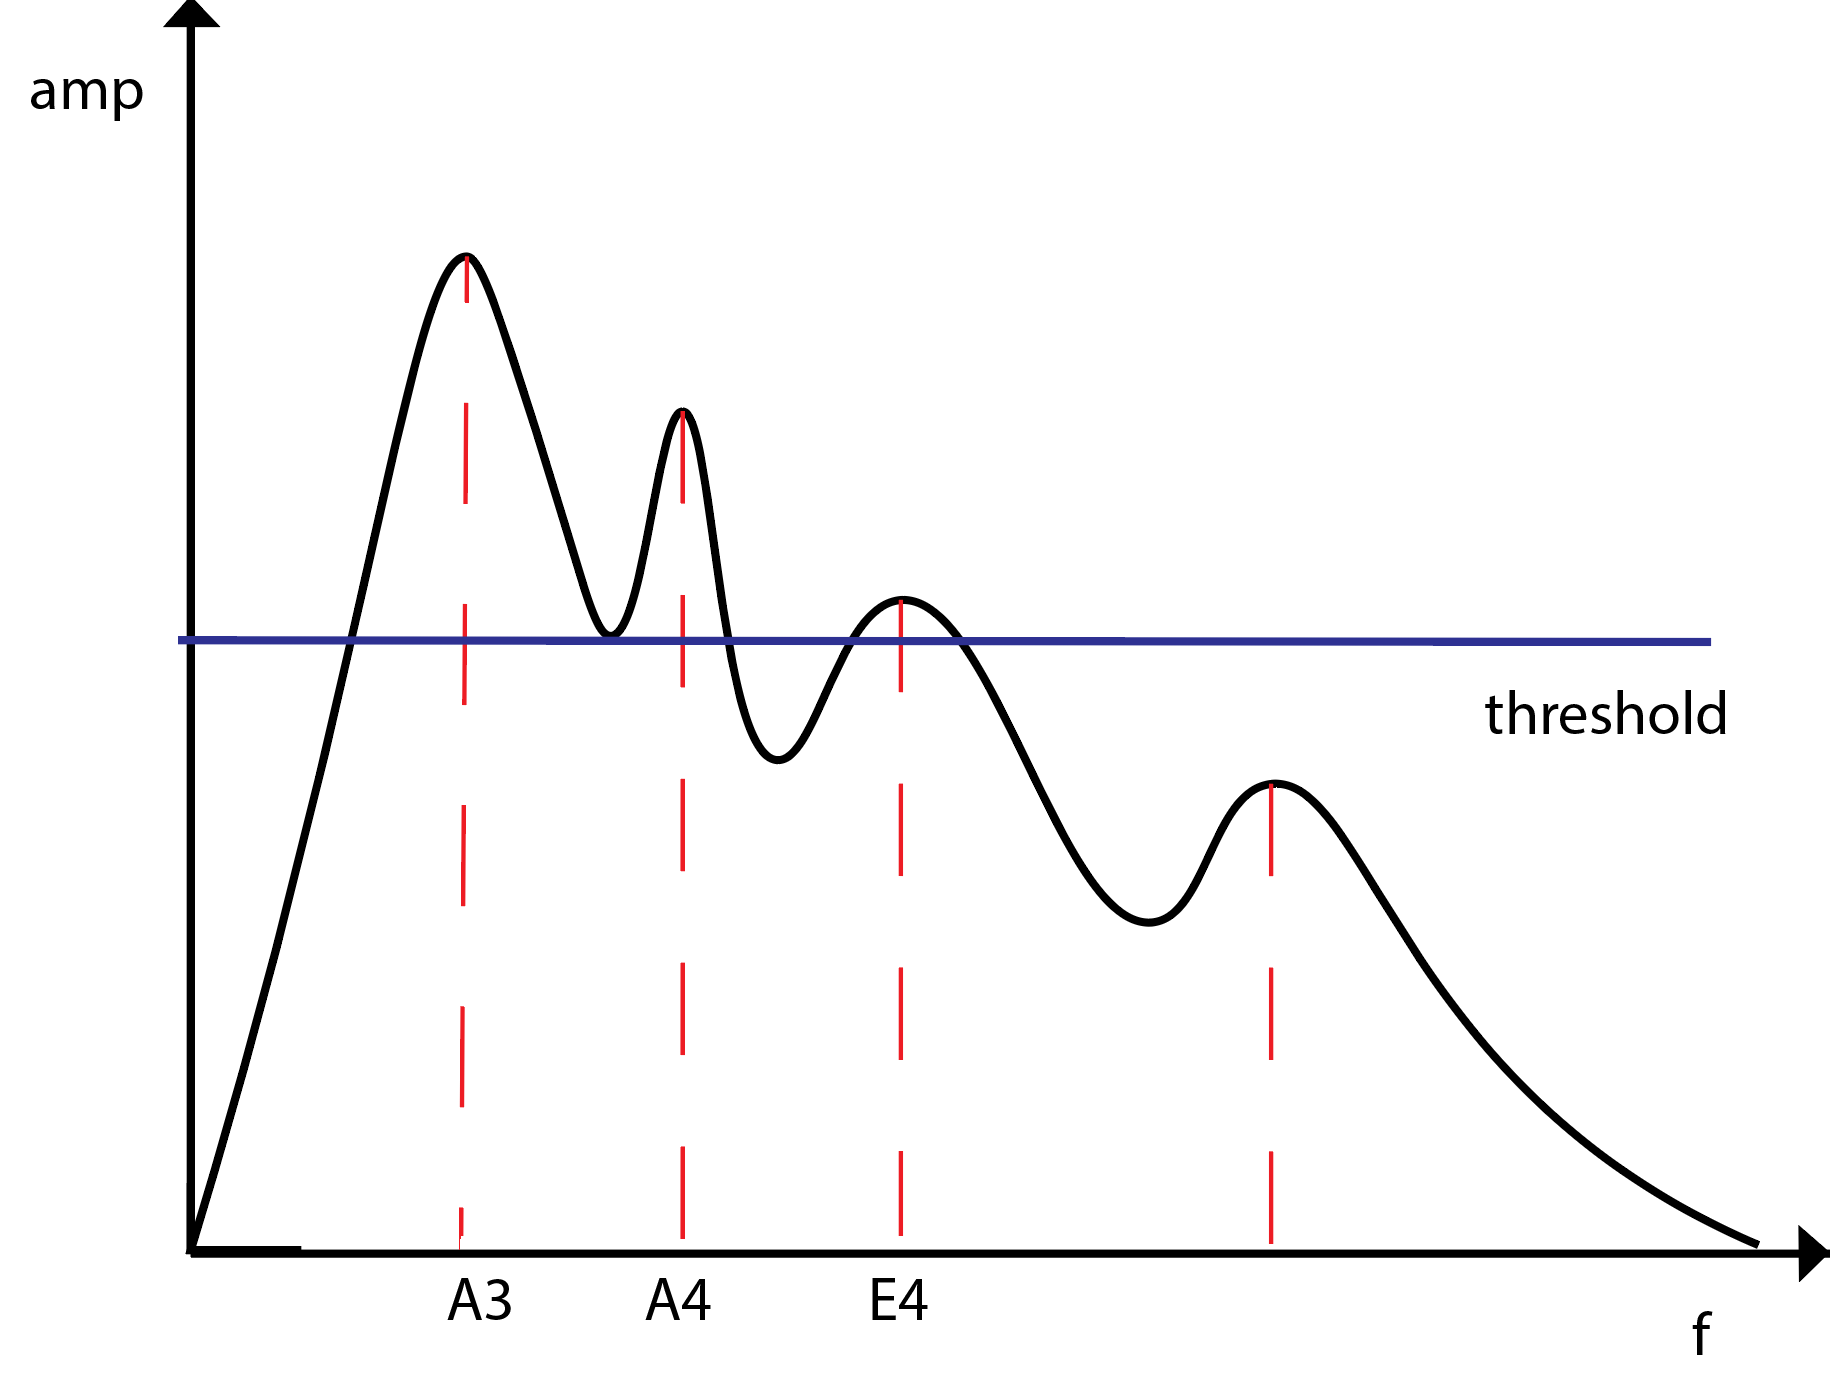
\includegraphics[scale=0.3]{harmofilter.png}
    \caption{Representation of the harmonic filter}
    \label{fig:harmofilter}
\end{figure}

(1) An \textbf{harmonic filter}. It is a filter that reduces the set of sounds in order to apply algorithms on smaller database and running faster. Looking at the spectral envelope of the static target sound, it is possible to extract the fundamental harmonic (the first partial) and its corresponding note as well as the other present harmonics and notes. The partials and their specific notes are represented by peaks in the spectral envelope. The partial filtering, i.e the harmonic filter, uses then a threshold applied on the spectral envelop and only keep in the database the notes corresponding to the peaks above the threshold. \\

Figure \ref{fig:harmofilter} illustrates the harmonic filter. In the example, the peaks above the threshold have corresponding notes/partials A3, A4 and E4. This implies that in the database will be present only sounds with the notes A3, A4 and E4, removing all the other notes for all instrument and reducing considerably the size of the database to use. \\


(2) \textbf{Upper and lower penalties} The distance measure $d(S,G)$ used in the software is actually not symmetric. For musical purpose, it is less problematic on a dimension to be lower than the target than higher than it regarding the amplitude of the spectral envelopes of both sounds. This induces a slight modification in the objective function.\\

Figure \ref{fig:penalt} is a representation of the penalties. The blue curve represents the spectral envelop of the target sound and the red one the solution envelop. Positive penalties (+) are applied when the solution curve peaks are below the target ones and negative penalties (-) when they are above the target spectral envelop. 

\begin{figure}[h!]
    \centering
    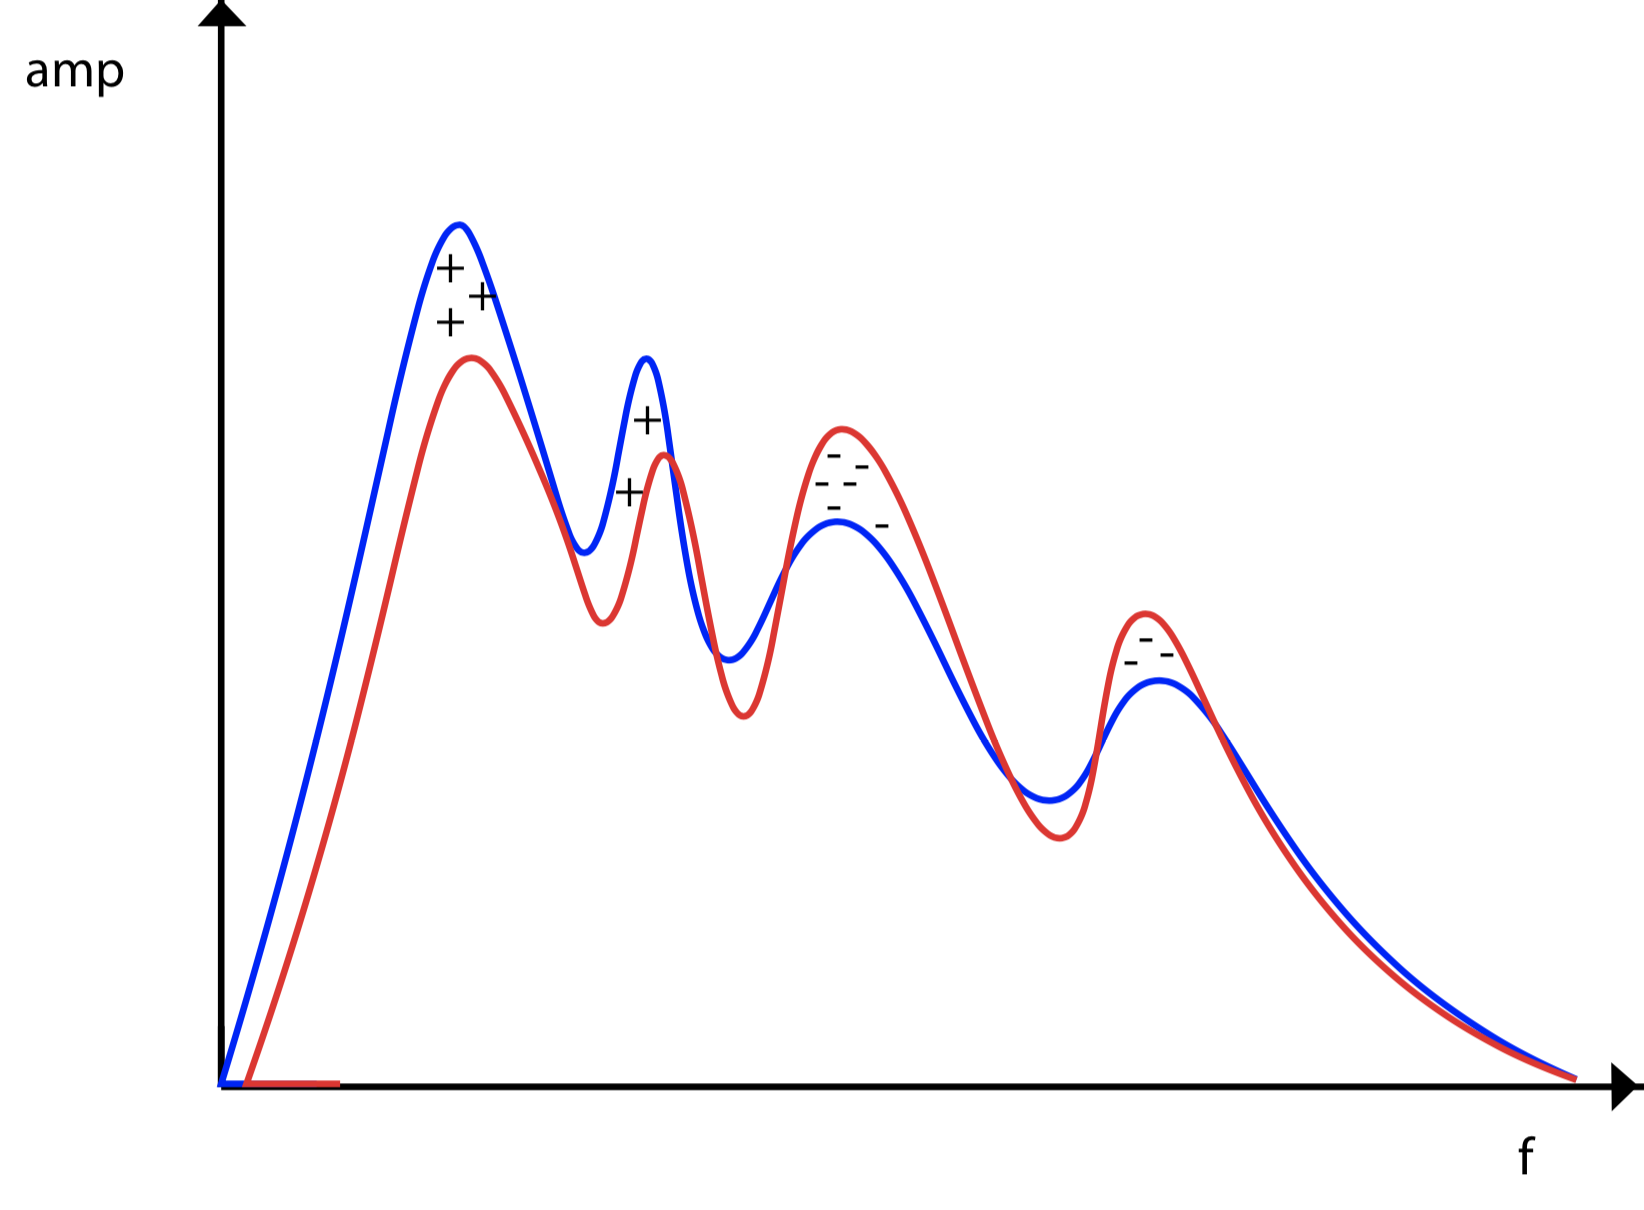
\includegraphics[scale=0.3]{penalt.png}
    \caption{Representation of the penalties with the blue curve the spectral envelop of the target sound and the red one the solution envelop}
    \label{fig:penalt}
\end{figure}

To make a fare comparison between with the solutions computed by the \textit{Orchidea} software and by the ILP, we chose to include these two ingredients in  ILP experiments, i.e., the calculations were applied on the same databases and with the same penalty factors.

For illustrative purpose Figure~\ref{fig:claA3} represents the target Clarinet A3 (in red) and its optimal solution (in blue). The horizontal axis represents frequencies, and the vertical axis the value in the spectral analysis. We see that the solution produces a sound which essentially uses the same frequencies. 

\begin{figure}[ht!]
    \centering
    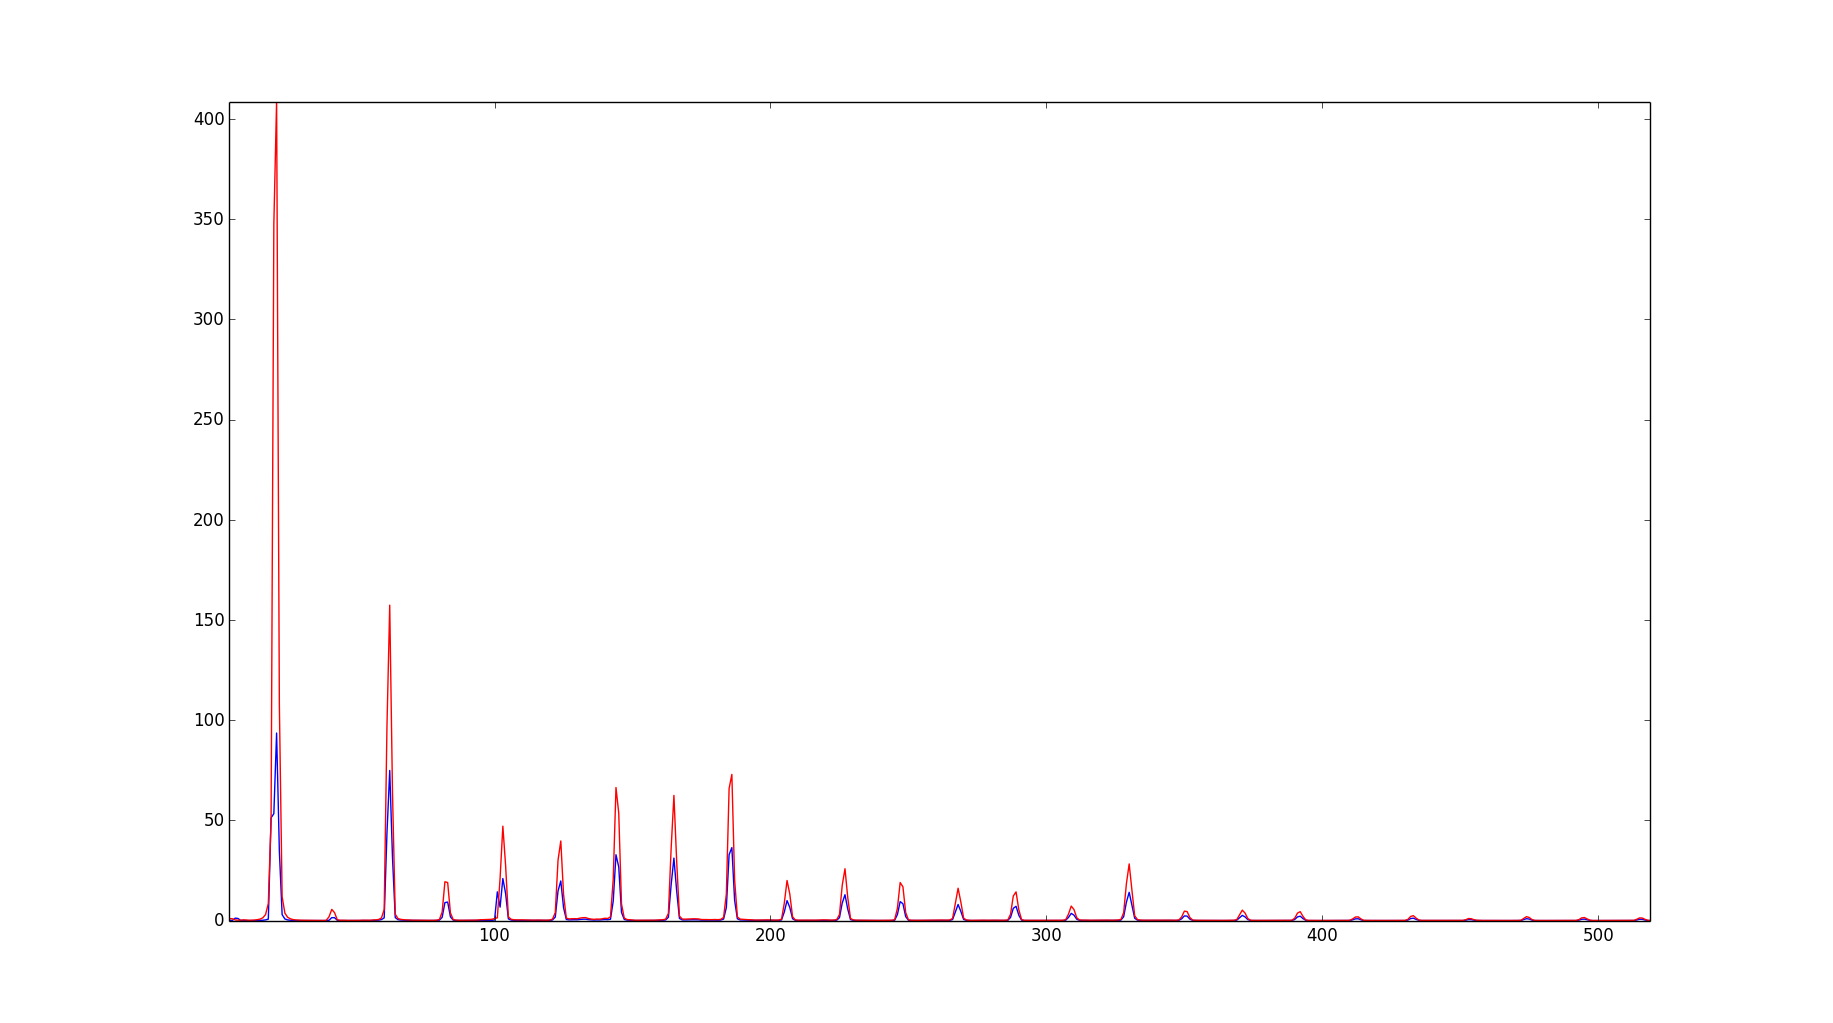
\includegraphics[scale=0.3]{clarinetA3.png}
    \caption{Representation of the solution with the static target Clarinet A3 }
    \label{fig:claA3}
\end{figure}

In Tabular \ref{tab:resultstat} are presented our results on some static targets sounds. The ILP was able to solve optimally all instances. Concerning the solutions themselves, it is noticeable that for some instances the two algorithms (note that \textbf{Evolutionnary} refers to the algorithm used in \textit{Orchidea}) chose disjoint sets of sounds. Concerning the values, ILP gives optimal solutions so the values are of course better, but we note that the improvements with respect to the solutions computed by the evolutionary algorithm are significant. These elements indicate that an LP approach is certainly interesting for the static orchestration problem. Even if the solution were better according to their values (calculated on the objective function of the ILP), some solutions of the evolutionary algorithm seemed to ``sound'' better. This is due to the hardness of the dissimilarity measure choice and to the ILP formulation being a simpler modelization than the evolutionary one. 
 

\begin{figure}[ht!]

\begin{center}
    \begin{tabular}{r||c|c}%{c|c|c|c|c}
     \textbf{target sound}&\textbf{ILP}&\textbf{Evolutionary}  \\
     \hline
     Archeos Bell&508&2803\\
Bass Clarinet&1114&6074\\
Beethoven Chord2&490&2401\\
Boat Docking&463&2363\\
Car Horn&1017&3968\\
Girl Scream&2651&3581\\
Winchester Bell&897&2302\\
Wind Harp&736&1656\\
YaBn mul PG ST12&757&5660\\	
\end{tabular}
\caption{Results of the ILP and the Evolutionary algorithms on some static target sounds.}

\label{tab:resultstat}
\end{center}
\end{figure}


In practice, there is a significant difference between the model and the reality. To overcome this difference and have results closer to real world applications, the script \textbf{dbgen} was developed in order to analyze the results. \textbf{dbgen} is a script that, given a sound or a set of sounds generates its feature description, i.e it creates a value vector of dimension the size of the chosen feature type (here 1024 as it is the spectrum feature that was used). \\
In the following tab results \ref{tab:resultstat2}, a sound was first generated based on the spectral description of the solution and then \textbf{dbgen} was applied to it, generating again a spectral description of the sound on which the distances were computed. \\
\begin{figure}[ht!]
\begin{center}
    

\begin{tabular}{r||c|c}%{c|c|c|c|c}
     \textbf{target sound}&\textbf{ILP post dbgen}&\textbf{Evolutionary post dbgen}  \\
    \hline
     Archeos Bell&3323&6436\\
Bass Clarinet&4785&14153\\
Beethoven Chord2&1145&2513\\
Boat Docking&1470&3922\\
Car Horn&1674&9414\\
Girl Scream&4096&4555\\
Winchester Bell&3097&3434\\
Wind Harp&3101&6288\\
YaBn mul PG ST12&1304&8255
 
\end{tabular}
\caption{Results of the ILP and the Evolutionary algorithms on some static target sounds using \textbf{dbgen}.}
\label{tab:resultstat2}
\end{center}
\end{figure}

Concerning the values of the tab \ref{tab:resultstat2}, ILP post dbgen still gives solutions with better values but it is interesting to notice that for most of the target sounds the solutions of the evolutionary algorithm and the ILP ones are much closer than in the previous tab.


\subsection{Dynamic Case}\label{sec:expdyn}

We give an ILP formulation of the assisted orchestration problem in its dynamic version. The idea behind the formulation is to emphasize the similarities and links with the multistage framework.\\
For the dynamic case, we now need to minimize $\sum_{t=1}^T d(S_t,G^t)+\sum_{t=1}^{T-1} C_t d(S_t,S_{t+1})$. 

% \begin{center}
%   \begin{eqnarray*}
%      \ \left \{ \begin{array}{ll}
%     \min \ \sum\limits_{i=1} ^ T d(S_i,G_i) +  \sum\limits_{i=2}^T B_i \text{ }d(S_i,S_{i-1}) \\
%     s.t. \left |
%     %\begin{array}{ll}
%     \begin{array}{llllll}
%     \sum\limits_{i \in N}  x_{ti} & \leq &L_t & \forall{t} \in \{1,...,T\} \\
 
%     x_{ti} \in \{0,1\} & & & \forall{t} \in \{1,...,T\}, \forall{i} \in N\\
%     %\end{array}\\
%     \end{array}
%     \right.
%     \end{array} 
%     \right.
%     \end{eqnarray*}
%     \end{center}

As said before, the function can be seen as a multistage framework function. \\
Indeed, one needs to seek a trade-off between:
\begin{itemize}
    \item the quality of the solution: on each of the $T$ time steps of the time horizon is computed a distance between the solution and the target sound
    \item the stability of the solution for consecutive time steps: for all consecutive time steps is computed the distance between the consecutive time steps solutions.
\end{itemize} 

Note that in our formulation of the problem, the distance to the target sound and the distance between consecutive time steps solutions is the same. The fact of using the same distance for the two ingredients of the objective function differs with the approach used in \textit{Orchidea} software. Indeed, a lot of different functions could be considered in order to evaluate the stability of a given solution to the problem. It could be interesting for example to seek a solution that minimizes: the instruments modifications (if an instrument is played at a time step $t$, a bonus is obtained for taking the same instrument at the next time step), the note modifications (keeping the same note on any instrument) or a combination of the two. This is interesting if a composer is giving importance to the continuity of its solutions (see \ref{fig:contmodel}) that is represented in the continuity model. Our choice of using the same distance measure gives us the possibility to model the problem as an ILP problem and not as a multi-objective problem, the two elements of our function being comparable. \\
Note also that in some cases, if the target pitch, i.e its notes, change a lot between two consecutive steps, it is not relevant to keep the same note as the result would be certainly far from the target sound. \\
%This possibility has been taken into account and model with bonus weighted in function of each target sound at each time step, i.e if the target does not change too much, the bonus is significant, if it does change a lot, the bonus would be less important.\\




Let us now focus on the ILP formulation. We need now to consider $nT$ binary variables $x_{it}$, indicating whether $s_i$ is taken in $S_t$ or not. To linearize the objective function, we can introduce $\Theta(nT)$ variables: $\delta_{jt}$ which will be equal to $|p_j(S_t)/|S_t|-G_j|$, and $\alpha_{jt}$ which will be equal to $|p_j(S_t)/|S_t|-p_j(S_{t+1})/|S_{t+1}||$. Then the objective is to minimize $\sum_{t=1}^T\sum_{j=1}^M \delta_{jt}+ \sum_{t=1}^{T-1}\sum_{j=1}^M \alpha_{jt}$, and we put the constraints:
\begin{itemize}
    \item $\delta_{jt}\geq \frac{p_j(S_t)}{|S_t|}-G_{jt}$ and $\delta_{jt}\geq G_{jt}-\frac{p_j(S_t)}{|S_t|}$;
    \item $\alpha_{jt}\geq \frac{p_j(S_t)}{|S_t|}-\frac{p_j(S_{t+1})}{|S_{t+1}|}$ and $\alpha_{jt}\geq \frac{p_j(S_{t+1})}{|S_{t+1}|}-\frac{p_j(S_t)}{|S_t|}$.
\end{itemize}

In order to linearize these constraints, as in the static case we can:
\begin{itemize}
    \item Either add some extra variables, to avoid quadratic terms in the constraints;
    \item Or fix the number of selected sounds at {\it each} time step, and solve the ILP for all the possible combinations of sizes of solutions $S_t$.
\end{itemize}
In the first case we need to introduce $\Omega(nMT)$ variables to linearize the constraints. In the second case we need to solve $L^T$ ILP, where $L$ is the maximum number of sounds selected at one time step, $L=23$ in our orchestra.

Both approaches were not able to solve our instances (recall that $n$ and $M$ are of order of 1000), as soon as $T>2$. 

% In order to model this dynamic problem as an ILP formulation we introduced a lot of new dummy variables.\\
% Indeed, let us introduce five dummy variables used in order to linearize the program:

% \begin{itemize}
%     \item $ \alpha_{ijt}= x_{it}\delta_{jt}$ 
%     \item $\beta_{it} = x_{i(t+1)}\sum\limits_{l\in N} x_{l(t)}$
%     \item $\lambda_{it} = x_{it}\sum\limits_{l\in N} x_{l(t+1)}$
%     \item $y_{ii't}= x_{it}x_{i'(t+1)}$ 
%     \item $\theta_{ii'tj}= y_{ii't} \gamma_{jt}$
% \end{itemize}


% We present the following linear program. The linear program is delimited into three programs of constraints, one for the "distances", one for the "linearization" of the variables and one for the "cardinality".\\
% The objective function of the linear program is:

% $\min \ \sum\limits_{t=1} ^ T \sum\limits_{j=1}^M \delta_{jt} + \sum\limits_{t=1}^{T-1} \sum\limits_{j=1}^M B_t \gamma_{jt}$

% with $\sum\limits_{t=1} ^ T \sum\limits_{j=1}^M \delta_{jt}$ being the distance of a solution to the target sound over the time horizon and $\sum\limits_{t=1}^{T-1} \sum\limits_{j=1}^M B_t \gamma_{jt}$ the distance measuring the stability of the solutions over the time horizon. 

% As said before, the program is subject to:\\
% The \textbf{"distances"} constraints:


% \begin{center}
%   \begin{eqnarray*}
%      \ \left \{ \begin{array}{ll}
%      \left |
%     \begin{array}{llll}
%     \sum\limits_{i\in N} \alpha_{ijt}+\sum\limits_{i \in N} x_{it}(p_{ij}-G_{jt})\geq 0& \forall{t} \in \{1,\ldots,T\},\forall{j} \in \{1,\ldots,M\} \\
%     \sum\limits_{i\in N} \alpha_{ijt}+\sum\limits_{i \in N} x_{it}(G_{jt}-p_{ij})\geq 0& \forall{t} \in \{1,\ldots,T\},\forall{j} \in \{1,\ldots,M\} \\
%     \sum\limits_{i \in N} \sum \limits_{i' \in N} \theta_{ii'tj}+\sum\limits_{i\in N} p_{ij}(\beta_{it}-\lambda_{it})\geq 0 & \forall j,\forall t \in \{1,\ldots,T-1\}\\
%   \sum\limits_{i \in N} \sum \limits_{i' \in N} \theta_{ii'tj}+\sum\limits_{i\in N} p_{ij}(\lambda_{it}-\beta_{it})\geq 0 & \forall j, \forall t \in \{1,\ldots,T-1\}\\
%     \end{array}
%     \right.
%     \end{array} 
%     \right.
%     \end{eqnarray*}
%     \end{center}

    
 
% The \textbf{"linearization"} constraints:


% \begin{center}
%   \begin{eqnarray*}
%      \ \left \{ \begin{array}{ll}
%      \\
%     s.t. \left |
%     %\begin{array}{ll}
%     \begin{array}{llll}
%   \alpha_{ijt} \geq \delta_{jt}-(1-x_{it})M& \forall i, \forall j, \forall t\\
%   \alpha_{ijt} \leq M x_{it} & \forall i, \forall j, \forall t\\
%   \alpha_{ijt} \geq 0 & \forall i, \forall j, \forall t\\
%   \alpha_{ijt} \leq \delta_{jt} & \forall i, \forall j, \forall t\\
%   y_{ii't} \geq x_{it} - (1-x_{i'(t+1)})M & \forall i, \forall i', \forall t \in \{1,\ldots,T-1\}\\
%   y_{ii't} \geq x_{i'(t+1)} - (1-x_{it})M & \forall i, \forall i', \forall t \in \{1,\ldots,T-1\}\\
%   y_{ii't} \leq x_{i'(t+1)} & \forall i, \forall i', \forall t \in \{1,\ldots,T-1\}\\
%   y_{ii't} \leq x_{it} & \forall i, \forall i', \forall t \in \{1,\ldots,T-1\} \\
%   y_{ii't} \geq 0 & \forall i, \forall i', \forall t \in \{1,\ldots,T-1\} \\
%   %y_{ii't} \leq x_{it} & \forall i, \forall i', \forall t \in \{1,\ldots,T-1\} \\
%   %y_{ii't} \leq x_{i'(t+1)} & \forall i, \forall i', \forall t \in \{1,\ldots,T-1\} \\
%   \theta_{ii'tj} \geq \gamma_{jt} - (1-y_{ii't})M & \forall i, \forall i', \forall j, \forall t \in \{1,\ldots,T-1\} \\
%   \theta_{ii'tj} \leq M y_{ii't} & \forall i, \forall i', \forall j, \forall t \in \{1,\ldots,T-1\} \\
%   \theta_{ii'tj} \geq 0 & \forall i, \forall i', \forall j, \forall t \in \{1,\ldots,T-1\} \\
%   \theta_{ii'tj} \leq \gamma_{jt} & \forall i, \forall i', \forall j, \forall t \in \{1,\ldots,T-1\} \\
%   \beta_{it}\leq \sum\limits_{\ell \in N} y_{\ell i t} & \forall i, \forall t \in \{1,\ldots,T-1\}\\
%   \beta_{it}\geq \sum\limits_{\ell \in N} y_{\ell i t}& \forall i, \forall t \in \{1,\ldots,T-1\}\\
   
   
%   \lambda_{it}\leq \sum\limits_{\ell \in N} y_{i \ell t} & \forall i, \forall t \in \{1,\ldots,T-1\}\\
%   \lambda_{it}\geq \sum\limits_{\ell \in N} y_{i \ell t}& \forall i, \forall t \in \{1,\ldots,T-1\}\\
   

%       \end{array}
%     \right.
%     \end{array} 
%     \right.
%     \end{eqnarray*}
%     \end{center}  

    
% and finnaly the \textbf{"cardinality"} constraints. Note the sounds are ordered by instruments in the database, i.e each sound is present in a fixed interval $I_z \subseteq N\  \forall z \in Z$:


% \begin{center}
%   \begin{eqnarray*}
%      \ \left \{ \begin{array}{ll}
%      \\
  
%     s.t. \left |
%     %\begin{array}{ll}
%     \begin{array}{llll}
   
%   \sum \limits_{i \in N} x_{it} \leq L_t & \forall t \\
%   \sum \limits_{i \in N_z} x_{it} \leq L_{zt} & \forall i, \forall t, \forall z\\
%     x_{it} \in \{0,1\} & \forall i, \forall{t} \\

    
%     %\end{array}\\
%     \end{array}
%     \right.
%     \end{array} 
%     \right.
%     \end{eqnarray*}
%     \end{center}
    
The number of variables of the linear program is very large, in fact there are: $NT$ variables $x$,$N^2T$ variables $y$,$MT$ variables $\delta$,$M(T-1)$ variables $\gamma$, $NMT$ variables $\alpha$, $N(T-1)$ variables $\beta$, $N(T-1)$ variables $\lambda$, $N^2(T-1)M$ variables $\theta$.

In practice, we apply the harmonic filter on the TinySol dataset and apply the algorithm on around $1400$ sounds, i.e $N=1400$, of dimension $M$ equal to $1024$ and it is possible to have around $20$ time steps, i.e $T=20$. The number of variables is thus extremly large. For exemple, only for the $\theta$ variable we have $1400^2 \times 20 \times 1024 = 40140800000 = 40$ billion $\theta$ variables. So it is impossible to run the program, even on powerful engines.  

However, to verify it, we runned the algorithm on a very restrictive instance with only $T=2$ time steps, a hard filter on the dataset, allowing only one note to be picken and thus around $N=250$ sounds, a small metric called moments with $M=4$. Even is this special case, the number of variables is quite large with around $2*250^2*4=500000$ $\theta$ variables. 




To overcome this difficulty, we rather propose in the following a heuristic, called {\it SPH}, the idea of which is to combine (1) the fact that we can solve the static problems (as explained in the previous section) (2) a shortest path formulation that allows to efficiently combine  solutions found in different time steps.  


\subsubsection{SPH: Shortest Path Heuristic}





In Theorems~\ref{th:dyn1dnoc} and~\ref{th:generaldynamic}, the principle was to use DP to produce a set of solutions at each time step, and then to solve a shortest path problem to find the best combinations of solutions. As explained previously, with $M=1024$ dimension we cannot use DP to produce solutions at each time step, but the shortest path idea is still interesting. Then, the principle of SPH (shortest path heuristics) is (see Figure \ref{fig:sph}):
\begin{itemize}
    \item To compute, for each time step $t$, a set $\Omega_t$ of feasible solutions;
    \item Then to find the best tuple $(S_1,\dots,S_T)\in \Omega_1\times \dots \times \Omega_T$, by solving a shortest path problem on a DAG on vertex set $\cup \Omega_t$ (and two vertices $s$ and $t$).
\end{itemize}

\begin{figure}[!ht]
\centering
\begin{tikzpicture}[scale=0.7,thick,
  every node/.style={draw,circle},
  fsnode/.style={fill=black},
  ssnode/.style={fill=black},
  every fit/.style={ellipse,draw,inner sep=-2pt,text width=1cm},
  ->,shorten >= 3pt,shorten <= 3pt
]

\begin{scope}[xshift=-2cm,yshift=-2.5cm,start chain=going below,node distance=7mm]
  %\node[ssnode,on chain] (s) [label=left:{a}] {};
  \node[ssnode,on chain] (s){};
\end{scope}

\begin{scope}[xshift=14cm,yshift=-2.5cm,start chain=going below,node distance=7mm]
  %\node[ssnode,on chain] (S) [label=right:{b}] {};
  \node[ssnode,on chain] (S) {};
\end{scope}

\begin{scope}[start chain=going below,node distance=7mm]
\foreach \i in {1,2,...,5}
  \node[fsnode,on chain] (f\i) [label=left: ] {};
\end{scope}	

\begin{scope}[xshift=3cm,,start chain=going below,node distance=7mm]
\foreach \i in {6,7,...,10}
  \node[ssnode,on chain] (s\i) [label=right: ] {};
\end{scope}

\begin{scope}[xshift=6cm,,start chain=going below,node distance=7mm]
\foreach \i in {11,12,...,15}
  \node[ssnode,on chain] (s\i) [label=right: ] {};
\end{scope}

\begin{scope}[xshift=9cm,,start chain=going below,node distance=7mm]
\foreach \i in {16,17,...,20}
  \node[ssnode,on chain] (s\i) [label=right: ] {};
\end{scope}

\begin{scope}[xshift=12cm,,start chain=going below,node distance=7mm]
\foreach \i in {21,22,...,25}
  \node[ssnode,on chain] (s\i) [label=right: ] {};
\end{scope}

% the set U
\node [black,fit=(f1) (f5),label=above:{$\Omega_1$}] {};
% the set V
\node [black,fit=(s6) (s10),label=above:{$\Omega_2$}] {};

\node [black,fit=(s11) (s15),label=above:{$\Omega_{\ldots}$}] {};

\node [black,fit=(s16) (s20),label=above:{$\Omega_{T-1}$}] {};
\node [black,fit=(s21) (s25),label=above:{$\Omega_T$}] {};




% the edges
\draw (f1) -- (s6);% node[midway,above] {$B$};
\draw (s) -- (f1);
\draw (s) -- (f2);
\draw (s) -- (f3);
\draw (s) -- (f4);
\draw (s) -- (f5);
\draw (s6) -- (s13);
\draw (s13) -- (s17);
\draw (s17) -- (s24);
\draw (s24) -- (S);

\end{tikzpicture}
\caption{Representation of the SPH algorithm for the D-TOP}
\label{fig:sph}
\end{figure}



The second step can be done very efficiently, and the problem boils down to finding interesting sets of solutions (independently) for each time step. \\
Recall that for the static case, we solve the instances using an ILP for each number of sounds $i$, from 1 to the maximum number of sounds $L$. This produces an interesting bunch of $L$ static solutions. Our heuristic SPH is precisely to use for $\Omega_t$ this set $A_t$ of $L$ feasible solutions. Once obtained these static solution, the shortest path problem is on $LT$ nodes (plus $s$ and $t$). \\
Note that overall the computation time is (nearly) linear in $T$.  


\subsubsection{Results on some dynamic target sounds}
As previously, we compare SPH with the solution output by the current software \textit{Orchidea}. 

%[Put results on SPH and \textit{Orchidea}, comments,...]

Also, we were interested in evaluating the choice of sets $\Omega_t=A_t$ in SPH. To do so, we also consider the set $E_t$ of solutions output by the evolutionary algorithm of \textit{Orchidea} on target at time $t$. We consider in the experiments 3 possible choices:
\begin{itemize}
    \item $\Omega_t=A_t$ (SPH);
    \item $\Omega_t=A_t\cup E_t$;
    \item $\Omega_t=E_t$.
\end{itemize}


\begin{figure}[ht!]
\centering
\begin{tabular}{c||c|c|c|c|c}%{c|c|c|c|c}
     \textbf{target sound}&$\Omega_t=A_t$&$\Omega_t=A_t\cup E_t$&$\Omega_t=E_t$  &\textit{Orchidea}&$T$\\
     \hline
A Minor&5354&5354&7236&8316&16\\
Brahms&3446&3446&4235&4845&8\\
Drops&5902&5902&8270&8925&12\\
Jarret Vienna&1727&1727&2304&2531&6\\

 
\end{tabular}
\caption{Summary of results of the LP and the Evolutionary algorithms on some static target sounds }
\label{tab:resultstat3}
\end{figure}

%[Again: description of the targets (and the orchestra), if not done before]


Figure~\ref{tab:resultstat3} shows the results we obtained for the dynamic instances, where $T$ is the number of time steps which go from 6 to 16. Here again SPH significantly improves the result on the computed solutions with respect to the current used heuristic - having in mind the same comments as previously on the accuracy of the model. We also note that the fact of adding $E_t$ in $\Omega_t$ never lead to an improvement of the result. The solutions output by the ILP at each time step seem to make a good set of individual solutions in SPH.


\section{Conclusion}

We provide in this chapter the first, to our knowledge, theoretical analysis of the static and dynamic target-based orchestration problems \stat and \dyn, showing both \textbf{NP}-hardness, pseudo-polynomial and approximation results. 
%[en dire plus?]






\chapterToc{Conclusion and outlook}

In this thesis we presented a wide variety of results for maximization optimization problems in the multistage framework and study a direct application of the multistage setting.\\ 

In the chapter \ref{chap:multiknap}, we presented a $PTAS$ for the {\sc multistage knapsack} problem in the offline setting. As an outlook, it would be interesting to address other maximization optimization problems in the offline setting, as the presence of an approximation scheme for the \textbf{NP}-hard {\sc knapsack} problem contrasts with inapproximability results for polynomial solvable problems in their classical version. Furthermore, we could try to understand the origin of the contrasts between optimization problems in their classical versions and in the multistage setting in order to be able to give a global characterization of multistage problems in the offline setting. \\

In the chapter \ref{chap:onlmultista}, we presented a framework of multistage subset maximization problems in the online setting looking at different models with different types of data evolution and transition bonus. An outlook would be to look at the family of multistage subset minimization problems and see if similar results are findable or not. \\
We also emphasize that we have focused on deterministic algorithms in this chapter. Indeed, some of our bounds can be improved by randomization (assuming an oblivious adversary):
\begin{itemize}
    \item In the general-evolution model with Hamming bonus assuming \finalversion{sub-additivity} and subset feasibility, there is a simple randomized $(2+o(1))$-competitive algorithm (along the lines of the algorithms in subsection~\ref{subsec:submodular}): Initially partition $N$ uniformly at random into two equal-sized sets (up to possibly one item) $A$ and $B$. At each time, select the optimal solution restricted to $A$. Again, the algorithm is $(2+o(1))$-competitive separately on both profit and bonus.
    \item While the strong lower bound without lookahead in the general-evolution model with intersection bonus still holds, we can get a simple $2$-competitive algorithm for lookahead $1$: Initially flip a coin to interpret the instance as a sequence of length-$2$ instances either starting at time $1$ or $2$. Thanks to lookahead $1$, the length-2 instances can all be solved optimally. The total value of all these length-2 instances adds up to at least the optimal value, and the expected value obtained by the algorithm is half of that.
\end{itemize}

While we believe that we have treated various of the most natural ways of defining value in multistage subset maximization problems, other ways can be thought of, to some of which our results extend. For instance, Theorem~\ref{thm:static-hamming-upper} also works for time-dependent or object-dependent bonus without major modifications (whereas, e.g., Theorem~\ref{thm:static-intersection-upper} does not).

We have not considered computational complexity in the is work assuming (and therefore neither about the representation of the set of feasible solutions); indeed, often we use an oracle providing the optimal solution to instances of a potentially hard problem. However, we mention that, if only an approximation algorithm to the problem at hand was known, we would be able to obtain similar online algorithms whose competitive ratio would depend on the approximation guarantee of the approximation algorithm.\\


Finally in the chapter \ref{chap:orche}, we gave the first theoretical analysis of the static and dynamic target-based orchestration problems. 
The experiments we conducted give hope for possible practical improvements using ILP and shortest path formulations. As said previously, this is only a first step in this direction - there is probably a gap between a good solution for the abstract model we consider and what a composer would consider as a harmonious solution - but a promising step. Also, if one manages to understand better the problem itself and especially to find a unique best dissimilarity measure between different sounds, it would be possible to decrease the difference between the abstract solution given by our model and the best solution from a composer standpoint.   



%\sectionToc{Contenu de ce document}
\chapterToc{BIBLIOGRAPHY}
\bibliographystyle{apalike}
\bibliography{biblio}


\end{document}




dynamic parameterized complexity
Dynamic Graph Algorithms Giuseppe F. Italiano\\
when a solution is taken the instance, edges or vertices change \\
DATA STRUCTURES FOR online UPDATING OF
MINIMUM SPANNING TREES, WITH APPLICATIONS*\\




There are two natural ways to define the transition bonus/cost in the case where the transition bonus/cost function is part of the objective function. We will see that these two ways of measuring the stability induce some differences in the results one can get. 


\begin{definition}
\emph{(Types of transition bonus/cost.)}
We can define the transition bonus/cost as:
\begin{itemize}
    \item \emph{Intersection Bonus/Cost:}  in this case the bonus/cost is proportional to the number of objects in the solution at time $t$ that remain in it at time $t+1$. In the previous example, the value of the bonus would be inferior, indeed we would get a bonus only for the object taken at both time steps but not for the objects not taken at both time steps.
    \item \emph{Hamming Bonus/Cost:} here we get the bonus/cost for each object for which the decision (to be in the solution or not) is the same between time steps $t$ and $t+1$. In other words, the bonus/cost is proportional to $|N|$ minus the number of modifications (Hamming distance) in the solutions. The \emph{Hamming Bonus} was presented previously in the {\sc multistage knapsack} problem example where we got some bonus for both objects taken and not taken at both time steps.
\end{itemize}
\end{definition}
aaa